\documentclass[12pt,spanish,fleqn,openany,letterpaper,pagesize]{scrbook}

\usepackage[utf8]{inputenc}
\usepackage[spanish]{babel}%escribir con acentos sin necesidad de comandos \'{} .
\usepackage{fancyhdr}
\usepackage{graphics}
\usepackage{epsfig}
\usepackage{epic}
\usepackage{eepic}
\usepackage{amsmath}
\usepackage{threeparttable}
\usepackage{amscd}
\usepackage{here}
\usepackage{graphicx}
\usepackage{lscape}
\usepackage{tabularx}
\usepackage{subfigure}
\usepackage{longtable}


\usepackage{rotating} %Para rotar texto, objetos y tablas seite. No se ve en DVI solo en PS. Seite 328 Hundebuch
                        %se usa junto con \rotate, \sidewidestable ....


\renewcommand{\theequation}{\thechapter-\arabic{equation}}
\renewcommand{\thefigure}{\textbf{\thechapter-\arabic{figure}}}
\renewcommand{\thetable}{\textbf{\thechapter-\arabic{table}}}


\pagestyle{fancyplain}%\addtolength{\headwidth}{\marginparwidth}
\textheight22.5cm \topmargin0cm \textwidth16.5cm
\oddsidemargin0.5cm \evensidemargin-0.5cm%
\renewcommand{\chaptermark}[1]{\markboth{\thechapter\; #1}{}}
\renewcommand{\sectionmark}[1]{\markright{\thesection\; #1}}
\lhead[\fancyplain{}{\thepage}]{\fancyplain{}{\rightmark}}
\rhead[\fancyplain{}{\leftmark}]{\fancyplain{}{\thepage}}
\fancyfoot{}
\thispagestyle{fancy}%


\addtolength{\headwidth}{0cm}
\unitlength1mm %Define la unidad LE para Figuras
\mathindent0cm %Define la distancia de las formulas al texto,  fleqn las descentra
\marginparwidth0cm
\parindent0cm %Define la distancia de la primera linea de un parrafo a la margen

%Para tablas,  redefine el backschlash en tablas donde se define la posici\'{o}n del texto en las
%casillas (con \centering \raggedright o \raggedleft)
\newcommand{\PreserveBackslash}[1]{\let\temp=\\#1\let\\=\temp}
\let\PBS=\PreserveBackslash

%Espacio entre lineas
\renewcommand{\baselinestretch}{1.1}

%Neuer Befehl f\"{u}r die Tabelle Eigenschaften der Aktivkohlen
\newcommand{\arr}[1]{\raisebox{1.5ex}[0cm][0cm]{#1}}

%Neue Kommandos
\usepackage{Befehle}
%Inicio del documento. Tener en cuenta que hay archivos auxiliares

\begin{document}
\pagenumbering{roman}
%\newpage
%\setcounter{page}{1}
\begin{center}
\begin{figure}
\centering%

\epsfig{file=HojaTitulo/EscudoUN,scale=1}%
\end{figure}
\thispagestyle{empty} \vspace*{1.0cm} \textbf{\LARGE
Un modelo ejecutable para la simulación multi-f\'{\i}sica de procesos de recobro mejorado en yacimientos de petr\'{o}leo basado en esquemas preconceptuales}\\[5.5cm]
\Large\textbf{Steven Velásquez Chancí}\\[5.5cm]
\small Universidad Nacional de Colombia\\
Facultad de Minas, Departamento de Ciencias de la Computación y la Decisión\\
Medellín, Colombia\\
2019\\
\end{center}

\newpage
\begin{center}
\thispagestyle{empty} \vspace*{0cm} \textbf{\LARGE
Un modelo ejecutable para la simulación multi-f\'{\i}sica de procesos de recobro mejorado en yacimientos de petr\'{o}leo basado en esquemas preconceptuales}\\[2.0cm]
\Large\textbf{Steven Velásquez Chancí}\\[2.0cm]
\small Tesis de investigación presentada como requisito parcial para optar al
t\'{\i}tulo de:\\
\textbf{Magíster en Ingeniería de Sistemas}\\[2.0cm]
Director:\\
Ph.D. Juan Manuel Mejía Cárdenas\\
Co-Director:\\
Ph.D. Carlos Mario Zapata Jaramillo\\[2.0cm]
L\'{\i}nea de Investigaci\'{o}n:\\
Ingeniería de Software\\
Grupos de Investigaci\'{o}n:\\
Dinámicas de Flujo y Transporte en medios porosos\\
Lenguajes Computacionales\\[2.0cm]
Universidad Nacional de Colombia\\
Facultad de Minas, Departamento de Ciencias de la Computación y la Decisión\\
Medellín, Colombia\\
2019\\
\end{center}

\newpage{\pagestyle{empty}\cleardoublepage}

\newpage
\thispagestyle{empty} \textbf{}\normalsize
\\\\\\%
~\\[4.0cm]

\begin{flushright}
\begin{minipage}{8cm}
    \noindent
        \small
        ~\\[2.0cm]
        A mi familia, Danna, amigos y a todos los que\\
        estuvieron pendientes de este proceso.\\
        ¡Se logró!
        
        %La preocupaci\'{o}n por el hombre y su destino siempre debe ser el
        %inter\'{e}s primordial de todo esfuerzo t\'{e}cnico. Nunca olvides esto
        %entre tus diagramas y ecuaciones.\\\\
        %Albert Einstein\\
\end{minipage}
\end{flushright}

\chapter*{Agradecimientos}
\addcontentsline{toc}{chapter}{\numberline{}Agradecimientos}
Agradezco a mi Director Juan Manuel Mejía Cardenas por su supervisión y confianza durante este proceso, a mi Codirector Carlos Mario Zapata Jaramillo por su guía y por saberme centrar cuando lo he requerido, a Juan David Valencia Londoño, cuya constante disposición para solucionar mis dudas me ayudaron a llevar un avance continuo, a Paola Andrea Nore\~{n}a Cardona, por su fé, apoyo, asesoría y acompañamiento constante durante el desarrollo de esta Tesis.\\

Finalmente, agradezco al Departamiento de Ciencias de la Computación y la Decisión por financiar mis estudios por medio de la beca de Facultad y a la alianza formada por el Departamento Administrativo de Ciencia, Tecnología e Innovación (COLCIENCIAS), la Agencia Nacional de Hidrocarburos (ANH) y la Universidad Nacional de Colombia por el financiamiento del ``Plan Nacional para el Potenciamiento de la Tecnología CEOR con Gas Mejorado Químicamente'' bajo el acuerdo 273-2017, dentro del cual se enmarca la investigación asociada a esta Tesis de Maestría.

\newpage{\pagestyle{empty}\cleardoublepage}

\chapter*{Resumen}
\addcontentsline{toc}{chapter}{\numberline{}Resumen}

La simulación de procesos de recobro mejorado se rige por las leyes en las que se describe el transporte de fluidos en medios porosos. Existen múltiples propuestas de elaboración de \textit{frameworks} y simuladores para procesos de recobro mejorado. Sin embargo, carecen de trazabilidad de conceptos, procesos y de representación de eventos que surgen de la física. En los Esquemas Preconceptuales (EP) se incluye toda la estructura de un dominio de aplicación y, también se pueden representar los procesos que se dan en tal dominio. Estos, aportan cohesión, consistencia y trazabilidad entre conceptos y procesos. Por lo que, en esta Tesis de Maestría se propone un modelo ejecutable para la simulación de procesos de recobro mejorado basado en esquemas preconceptuales. El modelo ejecutable se valida con el noveno \textit{SPE Comparative Solution Project}. Los resultados del modelo ejecutable se ajustan a los datos reportados en la literatura. El modelo ejecutable propuesto permite trazar consistentemente los conceptos, procesos y eventos presentes en la simulación de procesos de recobro mejorado.\\


\textbf{\small Palabras clave: Modelo Ejecutable, Esquemas Preconceptuales, Simulación de Yacimientos de Petróleo, Procesos de Recobro Mejorado, Representación Basada en Eventos}.\\

%El resumen es una presentaci\'{o}n abreviada y precisa (la NTC 1486 de 2008 recomienda revisar la norma ISO 214 de 1976). Se debe usar una extensi\'{o}n m\'{a}xima de 12 renglones. Se recomienda que este resumen sea anal\'{\i}tico, es decir, que sea completo, con informaci\'{o}n cuantitativa y cualitativa, generalmente incluyendo los siguientes aspectos: objetivos, dise\~{n}o, lugar y circunstancias, pacientes (u objetivo del estudio), intervenci\'{o}n, mediciones y principales resultados, y conclusiones. Al final del resumen se deben usar palabras claves tomadas del texto (m\'{\i}nimo 3 y m\'{a}ximo 7 palabras), las cuales permiten la recuperaci\'{o}n de la informaci\'{o}n.\\


%\textbf{\small Palabras clave: (m\'{a}ximo 10 palabras, preferiblemente seleccionadas de las listas internacionales que permitan el indizado cruzado)}.\\

%A continuaci\'{o}n se presentan algunos ejemplos de tesauros que se pueden consultar para asignar las palabras clave, seg\'{u}n el \'{a}rea tem\'{a}tica:\\

%\textbf{Artes}: AAT: Art y Architecture Thesaurus.

%\textbf{Ciencias agropecuarias}: 1) Agrovoc: Multilingual Agricultural Thesaurus - F.A.O. y 2)GEMET: General Multilingual Environmental Thesaurus.

%\textbf{Ciencias sociales y humanas}: 1) Tesauro de la UNESCO y 2) Population Multilingual Thesaurus.

%\textbf{Ciencia y tecnolog\'{\i}a}: 1) Astronomy Thesaurus Index. 2) Life Sciences Thesaurus, 3) Subject Vocabulary, Chemical Abstracts Service y 4) InterWATER: Tesauro de IRC - Centro Internacional de Agua Potable y Saneamiento.

%\textbf{Tecnolog\'{\i}as y ciencias m\'{e}dicas}: 1) MeSH: Medical Subject Headings (National Library of Medicine's USA) y 2) DECS: Descriptores en ciencias de la Salud (Biblioteca Regional de Medicina BIREME-OPS).

%\textbf{Multidisciplinarias}: 1) LEMB - Listas de Encabezamientos de Materia y 2) LCSH- Library of Congress Subject Headings.\\

%Tambi\'{e}n se pueden encontrar listas de temas y palabras claves, consultando las distintas bases de datos disponibles a trav\'{e}s del Portal del Sistema Nacional de Bibliotecas\footnote{ver: www.sinab.unal.edu.co}, en la secci\'{o}n "Recursos bibliogr\'{a}ficos" opci\'{o}n "Bases de datos".\\

\chapter*{Abstract}
\addcontentsline{toc}{chapter}{\numberline{}Abstract}
Enhanced oil recovery (EOR) processes simulation is governed by mass conservation laws. In such laws, flow, accumulation, sources and sinks phenomena in porous media are described. Multiple proposals for framework and simulation elaboration have been defined. However, they lack concepts and processes tracing and event representation for physical phenomena. Preconceptual Schemas (PS) are used for including the complete structure of an application domain and representing processes emerging in such a domain. Cohesion, consistency, and tracing between concepts and processes is obtained by using PS. In this MSc. Thesis an executable model for enhanced oil recovery processes simulation based on preconceptual schemas is proposed. The executable model is validated by running the ninth SPE Comparative Solution Project. The results are in accordance with data reported in the literature. The proposed executable model allows for tracing consistently the concepts, processes, and events, which are present in EOR processes simulation. \\

\textbf{\small Palabras clave: Executable Models, Preconceptual Schemas, Oil Reservoir Simulation, Enhanced Oil Recovery Processes, Event based Representation}.\\

%Es el mismo resumen pero traducido al ingl\'{e}s. Se debe usar una extensi\'{o}n m\'{a}xima de 12 renglones. Al final del Abstract se deben traducir las anteriores palabras claves tomadas del texto (m\'{\i}nimo 3 y m\'{a}ximo 7 palabras), llamadas keywords. Es posible incluir el resumen en otro idioma diferente al espa\~{n}ol o al ingl\'{e}s, si se considera como importante dentro del tema tratado en la investigaci\'{o}n, por ejemplo: un trabajo dedicado a problemas ling\"{u}\'{\i}sticos del mandar\'{\i}n seguramente estar\'{\i}a mejor con un resumen en mandar\'{\i}n.\\[2.0cm]
%\textbf{\small Keywords: palabras clave en ingl\'{e}s(m\'{a}ximo 10 palabras, preferiblemente seleccionadas de las listas internacionales que permitan el indizado cruzado)}\\

\renewcommand{\tablename}{\textbf{Tabla}}
\renewcommand{\figurename}{\textbf{Figura}}
\renewcommand{\listtablename}{Lista de Tablas}
\renewcommand{\listfigurename}{Lista de Figuras}
\renewcommand{\contentsname}{Contenido}


%\newcommand{\clearemptydoublepage}{\newpage{\pagestyle{empty}\cleardoublepage}}
\cleardoublepage
\addcontentsline{toc}{chapter}{Lista de figuras} % para que aparezca en el indice de contenidos
\listoffigures % indice de figuras

\cleardoublepage
\addcontentsline{toc}{chapter}{Lista de tablas} % para que aparezca en el indice de contenidos
\listoftables % indice de tablas

%\chapter*{Lista de s\'{\i}mbolos}
\addcontentsline{toc}{chapter}{\numberline{}Lista de s\'{\i}mbolos}
Esta secci\'{o}n es opcional, dado que existen disciplinas que no manejan s\'{\i}mbolos y/o abreviaturas.\\

Se incluyen s\'{\i}mbolos generales (con letras latinas y griegas), sub\'{\i}ndices, super\'{\i}ndices y abreviaturas (incluir s\'{o}lo las clases de s\'{\i}mbolos que se utilicen). Cada una de estas listas debe estar ubicada en orden alfab\'{e}tico de acuerdo con la primera letra del s\'{\i}mbolo.
\section*{S\'{\i}mbolos con letras latinas}
 \label{simbolos}
 \renewcommand{\arraystretch}{1.3}
%\begin{longtable}[l]{*{4}{>{$}l<{$}}p{9cm}}
\begin{longtable}[l]{>{$}l<{$}l>{$}l<{$}>{$}l<{$}}
%\begin{tabular}
\textbf{S\'{\i}mbolo}&\textbf{T\'{e}rmino}&\textbf{Unidad SI}&\textbf{Definici\'{o}n}\\[0.5ex]\hline
\endfirsthead%
\textbf{S\'{\i}mbolo}&\textbf{T\'{e}rmino}&\textbf{Unidad SI}&\textbf{Definici\'{o}n}\\[0.5ex]\hline
\endhead%
      A              &\'{A}rea                                   &\text{m}^{2}                         &\int\int dxdy\\%
      A_{\text{BET}} &\'{A}rea interna del s\'{o}lido                &\frac{\text{m}^{2}}{\text{g}}        &\text{ver DIN ISO 9277}\\%
      A_{\text{g}}   &\'{A}rea transversal de la fase gaseosa    &\text{m}^{2}                         &\text{Ec...}\\%
      A_{\text{s}}   &\'{A}rea transversal de la carga a granel  &\text{m}^{2}                         &\text{Ec...}\\%
      a              &Coeficiente                            &1                                    &\text{Ec...}\\%
      a              &Contenido de ceniza                    &1                                    &\frac{m_{\text{ceniza}}}{m_{\text{bm,0}}}\\%
      c              &Contenido de carbono                   &1                                    &\frac{m_{\text{C}}}{m}\\%
      c              &Longitud de la cuerda                  &\text{m}                             &\text{Figura...}\\
      c              &Concentraci\'{o}n de la cantidad de materia&\frac{\text{mol}}{\text{m}^{3}}      &\frac{n}{V}\\%
      D              &Di\'{a}metro                               &\text{m}                             &\\%
      E_{\text{A}}   &Energ\'{\i}a de activaci\'{o}n                  &\frac{\text{kJ}}{\text{mol}}         &\text{Ec....}\\%
      F              &Fracci\'{o}n de materia vol\'{a}til            &1                                    &\text{ver DIN 51720}\\%
      Fr             &N\'{u}mero de Froude                       &1                                    &\frac{\omega^{2}R}{g_{\text{0}}}\\%
      \overrightarrow{g}&Aceleraci\'{o}n de la gravedad          &\frac{\text{m}}{\text{s}^{2}}        &\frac{d^{2}\overrightarrow{r}}{dt^{2}}\\%
      H              &Entalp\'{\i}a                               &\text{J}                             &U+PV\\%
      H_{\text{o}}   &Poder calor\'{\i}fico superior              &\frac{\text{MJ}}{\text{kg}}          &\text{ver DIN 51857}\\%
      h              &Contenido de hidr\'{o}geno                 &1                                    &\frac{m_{\text{H}}}{m}\\%
      K              &Coeficiente de equilibrio              &1                                    &\text{Ec...}\\%
      L              &Longitud                               &\text{m}                             &DF\\%
      L              &Longitud del reactor                   &\text{m}                             &\text{Figura...}\\%
      m              &Masa                                   &\text{kg}                            &DF\\%
      \dot{m}        &Flujo de masa                          &\frac{\text{kg}}{\text{s}}           &\frac{m}{t}\\%
      n              &Velocidad de rotaci\'{o}n                  &\frac{\text{1}}{\text{s}}            &\frac{\omega}{2\pi}\\%
      n              &Cantidad de materia                    &\text{mol}                           &DF\\%
      P              &Presi\'{o}n                                &\text{Pa}                            &\frac{\vec{F}\cdot\vec{n}}{A}\\%
      Q              &Calor                                  &\text{kJ}                            &\text{1. $LT$}\\%
      T              &Temperatura                            &\text{K}                             &DF\\%
      t              &Tiempo                                 &\text{s}                             &DF\\%
      x_{\text{i}}   &Fracci\'{o}n de la cantidad de materia     &1                                    &\frac{n_{\text{i}}}{n}\\%
      V              &Volumen                                &\text{m}^{3}                         &\int{dr^{3}}\\%
      \vec{u}        &Velocidad                              &\frac{\text{m}}{\text{s}}            &(\frac{dr}{dt},r\frac{d\upsilon}{dt},\frac{dz}{dt})\\%
      w_{\text{i}}   &Fracci\'{o}n en masa del componente i      &1                                    &\frac{m_{\text{i}}}{m_{\text{0}}}\\%
      w_{\text{w,i}} &Contenido de humedad de la sustancia i &1                                    &\frac{m_{\text{\wasser}}}{m_{\text{i,0}}}\\%
      Z              &Factor de gases reales                 &1                                    &\frac{pv}{RT}\\%
\end{longtable}
\vspace{5ex}
\section*{S\'{\i}mbolos con letras griegas}

\begin{longtable}[l]{>{$}l<{$}l>{$}l<{$}>{$}l<{$}}
\textbf{S\'{\i}mbolo}&\textbf{T\'{e}rmino}&\textbf{Unidad SI}&\textbf{Definici\'{o}n}\\[0.5ex] \hline%
\endfirsthead%
\textbf{S\'{\i}mbolo}&\textbf{T\'{e}rmino}&\textbf{Unidad SI}&\textbf{Definici\'{o}n}\\[0.5ex] \hline%
\endhead%
\renewcommand{\arraystretch}{1.3}
 \label{simbolosg}
     \alpha_{\text{BET}}  &Factor de superficie                  &\frac{\text{m}^{2}}{\text{g}}   &(w_{\text{F,waf}})(A_{\text{BET}})\\%
     \beta_{\text{i}}     &Grado de formaci\'{o}n del componente i   &1                               &\frac{m_{\text{i}}}{m_{\text{bm,0}}}\\%
     \gamma               &Wandhaftreibwinkel (Stahlblech)       &1                               &\text{Secci\'{o}n...}\\
     \epsilon             &Porosidad de la part\'{\i}cula             &1                               &1-\frac{\rho_{\text{s}}}{\rho_{\text{w}}}\\%
     \eta                 &mittlere Bettneigungswinkel (St\"{u}rzen) &1                               &\text{Figura...}\\%
     \theta               &\'{A}ngulo de inclinaci\'{o}n de la cama      &1                               &\text{Figura...}\\
     \theta_{\text{O}}    &\'{A}ngulo superior de avalancha          &1                               &\text{Figura...}\\
     \theta_{\text{U}}    &\'{A}ngulo inferior de avalancha          &1                               &\text{Figura...}\\
     \kappa               &Velocidad de calentamientoe           &\frac{\text{K}}{\text{s}}       &\frac{dT}{dt}\\%
     \nu                  &Coeficiente estequiom\'{e}trico           &1                               &\text{ver DIN 13345}\\%
     \rho_{\text{b}}      &Densidad a granel                     &\frac{\text{kg}}{\text{m}^{3}}  &\frac{m_{\text{S}}}{V_{\text{S}}}\;(\text{Secci\'{o}n...})\\
     \rho_{\text{s}}      &Densidad aparente                     &\frac{\text{kg}}{\text{m}^{3}}  &\frac{m_{\text{F}}}{V_{\text{P}}}\;(\text{Secci\'{o}n...})\\
     \rho_{\text{w}}      &Densidad verdadera                    &\frac{\text{kg}}{\text{m}^{3}}  &\frac{m_{\text{F}}}{V_{\text{F}}}\;(\text{Secci\'{o}n...})\\
     \tau                 &Tiempo adimensional                   &1                               &\text{Ec....}\\%
     \Phi_{\text{V}}      &Flujo volum\'{e}trico                     &\frac{\text{m}^{3}}{\text{s}}   &\frac{\Delta V}{\Delta t}\\
     \omega               &Velocidad angular                     &\frac{1}{\text{s}}              &\frac{d\upsilon}{dt}\\

\end{longtable}


\section*{Sub\'{\i}ndices}
\begin{longtable}[l]{>{}l<{}l}
  \textbf{Sub\'{\i}ndice} & \textbf{T\'{e}rmino} \\[0.5ex] \hline%
  \endfirsthead%
  \textbf{Sub\'{\i}ndice} & \textbf{T\'{e}rmino} \\[0.5ex] \hline%
  \endhead%
\renewcommand{\arraystretch}{1.4}\label{simbolosg}

 bm&materia org\'{a}nica\\%
 DR&Dubinin-Radushkevich\\%
 E&Experimental\\%
 g&Fase gaseosa\\%
 k&Condensado\\%
 Ma&Macroporos\\%
 P&Part\'{\i}cula\\%
 p&Poro\\%
 p&Pirolizado\\%
 R&Reacci\'{o}n\\%
 t&Total\\%
 wf&Libre de agua\\%
 waf&Libre de agua y de ceniza\\%
 0&Estado de referencia\\%

\end{longtable}


\setlength{\extrarowheight}{0pt}


\section*{Super\'{\i}ndices}
\begin{longtable}[l]{>{}l<{}l}
  \textbf{Super\'{\i}ndice} & \textbf{T\'{e}rmino} \\[0.5ex] \hline%
  \endfirsthead%
  \textbf{Super\'{\i}ndice} & \textbf{T\'{e}rmino} \\[0.5ex] \hline%
  \endhead%
\renewcommand{\arraystretch}{1.4}\label{simbolosg}

 n &Coeficiente x\\%



\end{longtable}


\setlength{\extrarowheight}{0pt}


\section*{Abreviaturas}
\begin{longtable}[l]{>{}l<{}l}
  \textbf{Abreviatura} & \textbf{T\'{e}rmino} \\[0.5ex] \hline%
  \endfirsthead%
  \textbf{Abreviatura} & \textbf{T\'{e}rmino} \\[0.5ex] \hline%
  \endhead%
\renewcommand{\arraystretch}{1.4}\label{simbolosg}
 1.$LT$&Primera ley de la termodin\'{a}mica\\%
 $DF$    &Dimensi\'{o}n fundamental\\%
 $RFF$   &Racimos de fruta fresca\\%

\end{longtable}


\setlength{\extrarowheight}{0pt}
%\include{Resumen}%\newcommand{\clearemptydoublepage}{\newpage{\pagestyle{empty}\cleardoublepage}}
\pagenumbering{arabic}
% !TeX spellcheck = es_ES
\chapter{Introducci\'{o}n}

La simulación de yacimientos de petróleo es una aplicación del flujo de fluidos en medios porosos. En esta, se estudia a nivel macroscópico el desplazamiento de los fluidos a través de una roca porosa y, que se debe a cambios de presión y saturación, efectos gravitacionales, capilares, entre otros. Tales fenómenos se rigen por las leyes de conservación de la masa o el volumen, las cuales se describen como un sistema de ecuaciones diferenciales parciales acoplado.\\

Un modelo de simulación que se usa en la industria es el \textit{Black Oil Model} (BOM), en este se considera el transporte de tres fluidos que se caracterizan a condiciones de barril estándar y que tienen compresibilidad. En el BOM también se consideran términos de fuentes y sumideros, los cuales se modelan como pozos. La solución analítica del sistema que se describe es inviable, por lo que se requiere una solución númerica. Para ello, se discretiza el dominio espacial y se obtiene un sistema de ecuaciones algebraicas sobre una celda y su conjunto de caras. El sistema que resulta es no lineal y se resuelve aplicando Newton-Raphson \citep{atkinson2008introduction}.\\

Los Esquemas Preconceptuales (EP) son representaciones intermedias que sirven para establecer un punto común de comprensión entre un interesado y un analista de software \citep{zapata2007phd}. Estos, tienen elementos que permiten representar la estructura del dominio y los procesos o acciones que se dan en el mismo. \cite{JCalle} y, \cite{norena2018det} extienden la notación de los EP para contextos de software científico, los cuales tienen dominios de aplicación de mayor complejidad.\\

Los modelos matemáticos aparecen en todo esfuerzo de desarrollo de un simulador o \textit{framework} de simulación para procesos de recobro mejorado. Además de los modelos matemáticos, se elaboran otras representaciones en las que se muestran los conceptos, flujos de los procesos, pero no son trazables y carecen de elementos para representar eventos. Las propuestas que consideran la trazabilidad son específicas de la implementación de su respectivo \textit{framework} o simulación. Todo esto, confluye en que los simuladores de yacimientos para procesos de recobro mejorado se realicen de manera empírica.\\

\cite{norena2018timrep}, \cite{norena2018det}, \cite{norena2018ruido} y \cite{norena2018bs} exponen el potencial de los EP para representar diferentes dominios de aplicación en software científico. Se logra evidenciar que en sus representaciones se mantiene la cohesión entre los elementos presentes en cada dominio, conservando así, la trazabilidad entre conceptos. Adicionalmente, en las propuestas que se enuncian, se logra trazar todo el proceso en el mismo esquema.\\

En esta Tesis de Maestría se desarrolla un modelo ejecutable para la simulación multifísica de procesos de recobro mejorado en yacimientos de petróleo basado en esquemas preconceptuales. El modelo ejecutable consta de ocho conceptos principales, tres eventos en los que se procesa la simulación y múltiples funciones en las que se incluyen las porciones de la representación que se reutilizan. Posteriormente, se presenta la traducción de las porciones más representativas del modelo ejecutable a código C++.\\

Conforme a lo anterior, esta Tesis se estructura de la siguiente manera: en el Capítulo \ref{cap:Marco}, se presenta el marco teórico para la caracterización del dominio; en el Capítulo \ref{cap:Antecedentes} se plantea el problema y se definen los objetivos de esta Tesis; en el Capítulo \ref{cap:Solucion} se propone el modelo ejecutable para la simulación de procesos de recobro mejorado como solución al problema; en el Capítulo \ref{cap:Validacion} se valida el modelo ejecutable con un caso de literatura; finalmente, en el Capítulo \ref{cap:Conclusiones} se presentan las conclusiones y el trabajo futuro.\\





%En la introducci\'{o}n, el autor presenta y se\~{n}ala la importancia, el origen (los antecedentes te\'{o}ricos y pr\'{a}cticos), los objetivos, los alcances, las limitaciones, la metodolog\'{\i}a empleada, el significado que el estudio tiene en el avance del campo respectivo y su aplicaci\'{o}n en el \'{a}rea investigada. No debe confundirse con el resumen y se recomienda que la introducci\'{o}n tenga una extensi\'{o}n de m\'{\i}nimo 2 p\'{a}ginas y m\'{a}ximo de 4 p\'{a}ginas.\\
%
%La presente plantilla maneja una familia de fuentes utilizada generalmente en LaTeX, conocida como Computer Modern, espec\'{\i}ficamente LMRomanM para el texto de los p\'{a}rrafos y CMU Sans Serif para los t\'{\i}tulos y subt\'{\i}tulos. Sin embargo, es posible sugerir otras fuentes tales como Garomond, Calibri, Cambria, Arial o Times New Roman, que por claridad y forma, son adecuadas para la edici\'{o}n de textos acad\'{e}micos.\\
%
%La presente plantilla tiene en cuenta aspectos importantes de la Norma T\'{e}cnica Colombiana - NTC 1486, con el fin que sea usada para la presentaci\'{o}n final de las tesis de maestr\'{\i}a y doctorado y especializaciones y especialidades en el \'{a}rea de la salud, desarrolladas en la Universidad Nacional de Colombia.\\
%
%Las m\'{a}rgenes, numeraci\'{o}n, tama\~{n}o de las fuentes y dem\'{a}s aspectos de formato, deben ser conservada de acuerdo con esta plantilla, la cual esta dise\~{n}ada para imprimir por lado y lado en hojas tama\~{n}o carta. Se sugiere que los encabezados cambien seg\'{u}n la secci\'{o}n del documento (para lo cual esta plantilla esta construida por secciones).\\
%
%Si se requiere ampliar la informaci\'{o}n sobre normas adicionales para la escritura se puede consultar la norma NTC 1486 en la Base de datos del ICONTEC (Normas T\'{e}cnicas Colombianas) disponible en el portal del SINAB de la Universidad Nacional de Colombia\footnote{ver: www.sinab.unal.edu.co}, en la secci\'{o}n "Recursos bibliogr\'{a}ficos" opci\'{o}n "Bases de datos".  Este portal tambi\'{e}n brinda la posibilidad de acceder a un instructivo para la utilizaci\'{o}n de Microsoft Word y Acrobat Professional, el cual est\'{a} disponible en la secci\'{o}n "Servicios", opci\'{o}n "Tr\'{a}mites" y enlace "Entrega de tesis".\\
%
%La redacci\'{o}n debe ser impersonal y gen\'{e}rica. La numeraci\'{o}n de las hojas sugiere que las p\'{a}ginas preliminares se realicen en n\'{u}meros romanos en may\'{u}scula y las dem\'{a}s en n\'{u}meros ar\'{a}bigos, en forma consecutiva a partir de la introducci\'{o}n que comenzar\'{a} con el n\'{u}mero 1. La cubierta y la portada no se numeran pero si se cuentan como p\'{a}ginas.\\
%
%Para trabajos muy extensos se recomienda publicar m\'{a}s de un volumen. Se debe tener en cuenta que algunas facultades tienen reglamentada la extensi\'{o}n m\'{a}xima de las tesis  o trabajo de investigaci\'{o}n; en caso que no sea as\'{\i}, se sugiere que el documento no supere 120 p\'{a}ginas.\\
%
%No se debe utilizar numeraci\'{o}n compuesta como 13A, 14B \'{o} 17 bis, entre otros, que indican superposici\'{o}n de texto en el documento. Para resaltar, puede usarse letra cursiva o negrilla. Los t\'{e}rminos de otras lenguas que aparezcan dentro del texto se escriben en cursiva.\\

%%% Importancia de la investigación %%%
%Hablar de la industria del petróleo, de que tienen plata e investigan al respecto. Las reservas actuales, los procesos de recobro primario y secundario...
%Depletamiento

%Oil reservoir simulation has proven an usefull tool for predicting reserves and production along the years. A large quantity of studies have demonstrated the capacity of oil reservoir simulation for predicting the production of multiple reservoirs around the world .The simulation of such a problem consists of solving a coupled set of mass balance equations across a domain (reservoir, geometry - geological model). Therefore, the creation of oil reservoir simulators is in the scietific software research area (Rewrite). 

%%% Fenómenos complejos de EOR.

%Explicar por qué la simulación de yacimientos de procesos EOR se enmarca dentro del contexto del software científico.


%Hablar de que las operaciones de recobro mejorado son sensibles y que existen multiples casos en los que pueden fallar. (Hablar de asfaltenos quizá o polímeros)
%Daño de yacimiento
%Se requiere buen conocimiento de los fenómenos involucrados en los procesos EOR 
%Oil reservoir simulation consists of solving a set of coupled mass or moles balance equations, these equations are non-linear and need adecuate treatment in order to have a linear system that converges.

%Since the natural production is no longer maintainable, techniques of enhanced oil recovery (EOR) have been developed in order to mantain or even improve the recovery factor. These techniques involve the injection of chemicals that affect the rock and fluids properties making feasible to change the oil mobility and residual saturations... The EOR processes add new equations to the system that make the problem even bigger. Many authors have addressed this problem by making general flow simulation frameworks. Those frameworks implement the general workflow of solving the coupled set of equations generated by the phenomena in the reservoir.

%Some efforts have been done in the scientific software representation. Nore\~{a} et al. extend the preconceptual schema syntax defined by Zapata, 2007. for taking into account the elements needed in the scientific software context. Chaverra, 2011 includes cycles and conditional selection in the preconcpetual schema. Calle, 2017 defines design patterns in the context of scientific software using preconceptual schemas also extending its syntax.


%The existing frameworks vary in implementation, even though they apply the same techniques. This is due to the fact that design decisions are delegated to the programmer, which is an expert of flow in porous media simulation. Little effort has been done in representing the domain of reservoir simulation as is, including both dynamics and structure in the same representation. The existing studies in oil reservoir simulation domain representation lack of grouping the structural design with the dynamical behaviour. Others implement directly a solution of the set of differential equations for the specific study case. The problem knowledge is not shareable. The representations existing only account for the structural or, exclusively the dynamical behavior of the tool they developed. The use of the concepts lacks generality. Even though the formal definition of the differential equations, they lack information of constitutive equations. 

%In this thesis we propose an event based representation of the enhanced oil recovery simulation using preconceptual schemas. In order to do that, For this purpose. we describe the black oil simulation domain in the preconceptual schema syntax, later we define a generic component with both variable kinetical behavior and the capacity to change the flow properties in each phase. The developed model couples the models used for an enhanced oil recovery process in a preconceptual schema that represents adecuately the oil reservoir simulation domain, the representation is validated with the SPE Comparative solution project having accordance with the reported results.
%\chapter{Cap\'{\i}tulo 1}
%Los cap\'{\i}tulos son las principales divisiones del documento. En estos, se desarrolla el tema del documento. Cada cap\'{\i}tulo debe corresponder a uno de los temas o aspectos tratados en el documento y por tanto debe llevar un t\'{\i}tulo que indique el contenido del cap\'{\i}tulo.\\
%
%Los t\'{\i}tulos de los cap\'{\i}tulos deben ser concertados entre el alumno y el director de la tesis  o trabajo de investigaci\'{o}n, teniendo en cuenta los lineamientos que cada unidad acad\'{e}mica brinda. As\'{\i} por ejemplo, en algunas facultades se especifica que cada cap\'{\i}tulo debe corresponder a un art\'{\i}culo cient\'{\i}fico, de tal manera que se pueda publicar posteriormente en una revista.\\
%
%\section{Subt\'{\i}tulos nivel 2}
%Toda divisi\'{o}n o cap\'{\i}tulo, a su vez, puede subdividirse en otros niveles y s\'{o}lo se enumera hasta el tercer nivel. Los t\'{\i}tulos de segundo nivel se escriben con min\'{u}scula al margen izquierdo y sin punto final, est\'{a}n separados del texto o contenido por un interlineado posterior de 10 puntos y anterior de 20 puntos (tal y como se presenta en la plantilla).\\
%
%\subsection{Subt\'{\i}tulos nivel 3}
%De la cuarta subdivisi\'{o}n en adelante, cada nueva divisi\'{o}n o \'{\i}tem puede ser se\~{n}alada con vi\~{n}etas, conservando el mismo estilo de \'{e}sta, a lo largo de todo el documento.\\
%
%Las subdivisiones, las vi\~{n}etas y sus textos acompa\~{n}antes deben presentarse sin sangr\'{\i}a y justificados.\\
%
%\begin{itemize}
%\item En caso que sea necesario utilizar vi\~{n}etas, use este formato (vi\~{n}etas cuadradas).
%\end{itemize}

\chapter{Marco teórico}\label{cap:Marco}
%
%\section{Black Oil Model}

\section{El medio poroso}\label{sec:porousmedium}

La física en que se apoya la simulación de yacimientos de petróleo incluye el concepto de medio poroso. Un medio poroso se puede entender como un dominio espacial que ocupa parcialmente un sólido y una porción que ocupan los fluidos, a la que se le llama espacio vacío o poroso. Un yacimiento es un medio poroso que ocurre naturalmente, una formación geológica del subsuelo, que, a nivel microscópico, se compone por una red de poros que se pueden interconectar y que permiten almacenar fluidos \citep{Bear2018}.\\

La definición de medio poroso se extiende de la definición de un medio continuo. Un medio continuo, es aquel que no pierde sus propiedades cuando se divide infinitamente, es decir, sus propiedades son continuas en todo punto. Sin embargo, esta definición depende del nivel de observación. A nivel microscópico, si se toman medidas de espacio poroso en diferentes puntos, es posible encontrar unas zonas vacías y otras ocupadas por la roca. Por otro lado, al incrementar el tamaño de la muestra para la medida, es posible notar que las medidas toman valores menos oscilatorios, tal como se muestra en la Figura \ref{fig:medioporoso}. El mínimo tamaño de muestra al que el espacio poroso empieza a tomar un valor constante se le llama volumen de elemento representativo (REV, \cite{Bear2018}). El espacio poroso medido en un REV se denota porosidad ($\phi$), que corresponde a la capacidad de almacenamiento de fluidos a nivel macroscópico.\\

\begin{figure}[h]
	\centering%
	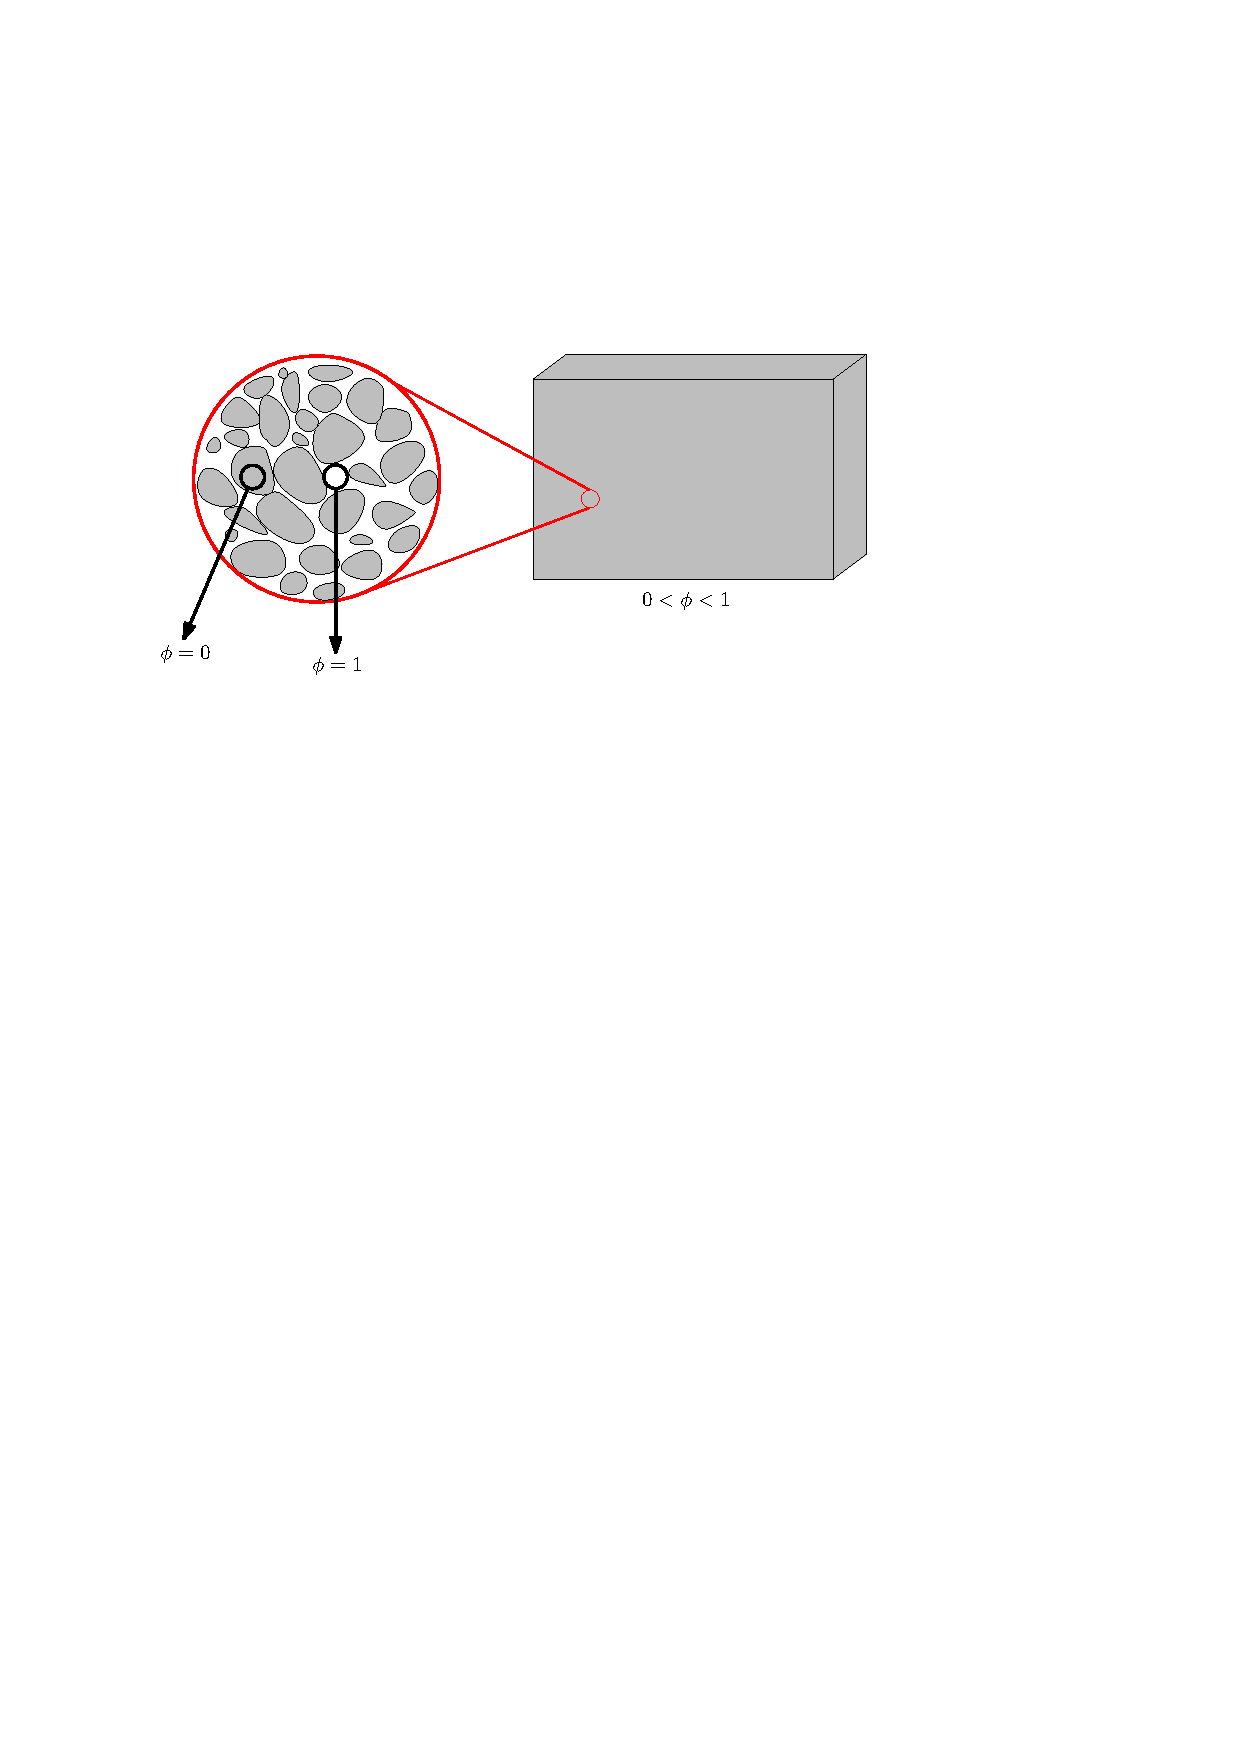
\includegraphics[scale=0.8]{Fig/porous_media.pdf}%
	\caption[Medio poroso y volumen de elemento representativo.]{Medio poroso y volumen de elemento representativo. Elaboración a partir de \cite{Bear2018}.} \label{fig:medioporoso}
\end{figure}
%Adicionalmente, existen gargantas de poro que conectan los poros de la roca, estas gargantas de poro indican la capacidad de la roca de permitir el transporte de los fluidos que puedan existir. La propiedad macroscópica que describe de la capacidad de transportar fluido es la permeabilidad absoluta. La permeabilidad absoluta es una propiedad direccional, es decir que puede variar según la dirección en la que se mida, si la permeabilidad varía su dirección en función del espacio, se dice que el medio es anisotrópico.

\section{Transporte de fluidos en medios porosos}\label{sec:Darcy}

Los fluidos que se almacenan en un yacimiento, en general, se encuentran en un estado estable, el cual se afecta con la aplicación de diferentes campos actuando sobre el dominio físico (el medio poroso). Así, los fluidos se pueden desplazar debido a efectos gravitacionales, cambios de presión y saturación o capilaridad, entre otros.\\ %En esta tesis de maestría se estudia el flujo o transporte dominado por la advección, es decir, el flujo que se da principalmente por gradientes de presión.

El flujo macroscópico de los fluidos se rige por la ley de conservación de momentum en medios porosos o ley de Darcy que se enuncia en la ecuación \ref{ec:DarcyMonofasico}. En esta ley se establece que la velocidad Darcy ($\vec{u}$) de un fluido es proporcional a los gradientes de presión y gravitacionales ($\nabla{\Phi}$ con $\Phi = p + \rho g z$) de un fluido, e inversamente proporcional a su viscosidad ($\mu$). Además, depende de la conductividad del medio poroso, a la cual se le denomina permeabilidad absoluta ($\mathbb{K}$) \citep{Whitaker1986, FANCHI2002108}.
\begin{align}
	\label{ec:DarcyMonofasico} & \vec{u}=\frac{\mathbb{K}}{\mu } \left(\nabla{\Phi}\right)	
\end{align}

%con $\nabla{\Phi_{f}} = \nabla{p} - \rho g \nabla{z}$ 

donde $\mathbb{K}(\vec{x},t)$ es una propiedad direccional con $\vec{x}=(x,y,z)$:
 
\begin{align}
	\mathbb{K} = \left(\begin{array}{ccc}k_{xx}& & \\
	& k_{yy} & \\
	& & k_{zz}
	\end{array}\right)
\end{align}

Estas ecuaciones se aplican para un solo fluido. En el caso de múltiples fluidos ocupando el espacio poroso se usa la ecuación \ref{ec:DarcyMultifasico}, en la cual, se introduce un término de permeabilidad relativa ($kr_{f}(S_{f})$), que depende de la fracción del volumen poroso que ocupa un fluido, la cual se denomina saturación ($S_{f}$).

\begin{align}
\label{ec:DarcyMultifasico} & \vec{u_{f}}=\frac{\mathbb{K}kr_{f}}{\mu_{f} } \nabla{\Phi_{f}}
\end{align}

\subsection{Mojabilidad}\label{subsec:Wettability}
En la mojabilidad se mide la preferencia de la superficie de una roca cuando se moja por determinado fluido o por una combinación de fluidos (mojabilidad intermedia) \citep{chen2007reservoir}. El fluido de preferencia o ``fluido mojante'' se atrapa en los poros más pequeños de la roca, generando una capa del fluido sobre la superficie de la misma \citep{chen2007reservoir}. A la fracción del fluido que se queda atrapado en la roca se le denomina ``saturación irreducible'' ($S_{fc}$) \citep{chen2007reservoir}. \\

\subsection{Presión Capilar}\label{subsec:Capillary}
Cuando existe flujo de dos fluidos, se genera una discontinuidad en la presión de ambos, la cuál se denomina ``presión capilar''. Ésta se calcula como la resta de la presión del ``fluido no mojante'' con la del ``fluido mojante''\citep{chen2007reservoir, FANCHI2002108}. En la Ecuación \ref{ec:presioncapilar} se presenta el cálculo de la ``presión capilar''.

\begin{align}
	\label{ec:presioncapilar}&p_c = p_{\text{fluido no mojante}} - p_{\text{fluido mojante}}
\end{align}\\

La presión capilar es función de la saturación de uno de los fluidos que se relaciona, según el caso: $p_c(S_{f})$. En el caso de un sistema de tres fluidos, se requieren dos presiones capilares \citep{chen2007reservoir}.

\subsection{Permeabilidad Relativa}\label{subsec:Krs}
La permeabilidad relativa ($k_{r}$) es una relación o fracción de movimiento de un fluido respecto a otro u otros \citep{chen2007reservoir}. Cuando sólo existen dos fluidos, la permeabilidad relativa es función directa de la saturación del fluido correspondiente ($k_{rf}(S_{f})$). Sin embargo, cuando hay tres o más fluidos, ésta puede depender de otras saturaciones ($k_{rf}(S_{f}, ...)$) \citep{chen2007reservoir}.

Cuando existen tres fluidos en un yacimiento de petróleo, obtener información experimental que relacione la permeabilidad relativa conjunta es difícil. En práctica, lo que se hace es medir permeabilidades relativas entre dos fluidos, es decir, los ``contactos'', e interpolar la permeabilidad del fluido de mojabilidad intermedia entre ellas. \citep{Zuo2014}.\\

Existen múltiples métodos de interpolación para obtener la permeabilidad relativa del fluido con más de un contacto \citep{Delshad1989, Blunt2000, Zuo2014}. Para el desarrollo de esta Tesis de Maestría se usa la interpolación de \cite{Baker1988}, la cuál se muestra en la Ecuación \ref{ec:Baker}.

\begin{align}
	\label{ec:Baker}&k_{ro}(S_{g}, S_{w}) = \frac{\left(S_{w}-S_{wc}\right)k_{row} + \left(S_{g}-S_{gc}\right)k_{rgo}}{\left(S_{w}-S_{wc}\right) + \left(S_{g}-S_{gc}\right)}
\end{align}\\

En un sistema de agua, gas y petróleo, se obtiene la permeabilidad relativa del petróleo al agua $k_{row}(S_{w})$ y la permeabilidad relativa del petróleo al gas $k_{rgo}(S_{g})$ y se pondera la permeabilidad relativa del petróleo por la saturación del gas y del agua \citep{Baker1988}.

\section{Simulación de Yacimientos de Petróleo}\label{sec:Simulation}
El dominio de la simulación de yacimientos de petróleo se enmarca dentro del contexto del desarrollo de software científico referido a procesos industriales y de investigación de nuevas tecnologías \citep{Kelly2015}; los cuales requieren la implementación de modelos matemáticos complejos que representan múltiples fenómenos físicos y químicos entre los fluidos. La simulación de yacimientos de petróleo se rige por las leyes de conservación de la masa y del momentum. En estas leyes se describe la acumulación, transporte, fuentes y sumideros de los fluidos como un sistema de ecuaciones diferenciales parciales acopladas para un dominio físico. La solución analítica de estos sistemas, cuando es viable, requiere condiciones que se alejan de los problemas reales \citep{ertekin2001basic}. Por ello, es necesario una solución numérica o simulación. Un modelo de simulación que se usa en la industria es el \textit{Black Oil Model}.%, este hace una simplificación de la composición de los hidrocarburos existentes. Solucionar tales ecuaciones requiere discretizar el tiempo y el dominio físico; usar métodos de solución de sistemas no lineales, y métodos de solución de sistemas lineales así como el precondicionamiento de los mismos. \\ %Estas elecciones tienen un impacto en las capacidades de solución de ecuaciones que surgen de los diferentes problemas físicos.\\
%Más aún, los resultados de la simulación deben ser contrastados con datos experimentales para verificar su concordancia con el fenómeno físico que modelan.\\


\subsection[Modelo \emph{Black Oil} Extendido]{Modelo {\normalfont \bfseries \itshape Black Oil} Extendido}\label{subsec:BOM}

El \textit{Black Oil Model} (BOM) es un modelo de conservación de volumen a condiciones estándar, en el cual, se considera la existencia de tres fluidos en el medio poroso: aceite, gas y agua. En el BOM, se asume que el aceite o petróleo tiene condiciones de barril estándar, es decir, presión y temperatura atmosférica \citep{chen2007reservoir}. Además, se supone que no existen variaciones considerables en la composición del aceite y del gas \citep{jamal2006petroleum, chen2007reservoir, ertekin2001basic}. En éste modelo se considera que puede existir una transferencia de masa en equilibrio desde aceite al gas, lo que se denomina ``Gas disuelto''. Adicionalmente, en el modelo \textit{Black Oil} extendido, se considera una transferencia de masa desde el gas al aceite, lo que se denomina ``aceite volatilizado''. Las siguientes son las ecuaciones de conservación de volumen del BOM \citep{jamal2006petroleum, chen2007reservoir, ertekin2001basic}.

\begin{align}
\label{ec:aceite}
\text{aceite: }&\frac{\partial}{\partial t} \left[ \phi \left( \frac{S_{o}}{B_{o}} + \frac{R_{v} S_{g}}{B_{g}} \right) \right]
- \nabla \cdot \left( \frac{1}{B_{o}} \vec{u_{o}} + \frac{R_{v}}{B_{g}} \vec{u_{g}} \right) + \tilde{q}_{o}=0  \\
\label{ec:gas}
\text{gas: }&\frac{\partial}{\partial t} \left[ \phi \left( \frac{S_{g}}{B_{g}} + \frac{R_{s} S_{o}}{B_{o}} \right) \right]
- \nabla \cdot \left( \frac{1}{B_{g}} \vec{u_{g}} + \frac{R_{s}}{B_{o}} \vec{u_{o}} \right) + \tilde{q}_{g} = 0 \\
\label{ec:agua}
\text{agua: }&\frac{\partial}{\partial t} \left[\phi \left( \frac{S_{w}}{B_{w}} \right) \right] - \nabla \cdot \left( \frac{1}{B_{w}} \vec{u_{w}} \right) + \tilde{q}_{w} = 0 
\end{align}
donde $\vec{u_{f}}$ corresponde a la velocidad Darcy y $\tilde{q}_{f}$ a los aportes de fuentes y sumideros, que posteriormente se modelan como pozos, para el fluido $f = \left\lbrace o:\text{ aceite}, g:\text{ gas}, w:\text{ agua} \right\rbrace $.\\

En el BOM se establece, también, que los fluidos tienen una compresibilidad, es decir que cambian su volumen y densidad debido a cambios de presión o transferencia de masa a otros fluidos (gas). La propiedad que se asocia a ese cambio de volumen es el factor volumétrico ($B_{f}$) \citep{chen2007reservoir}.\\

Para calcular las densidades del gas y del aceite en el BOM extendido, que se requieren en el cálculo de potencial de cada fluido, se tiene en cuenta la masa existente de aceite en el gas y viceversa. Para esto, se mide una densidad a condiciones estándar y se aplican la siguientes ecuaciones:

\begin{align}
	\label{ec:oildensity}&\rho_{o} = \frac{\rho_{o,sc} + R_{s}\rho_{g,sc}}{B_{o}}\\
	\label{ec:gasdensity}&\rho_{g} = \frac{\rho_{g,sc} + R_{v}\rho_{o,sc}}{B_{g}}\\
	\label{ec:watdensity}&\rho_{w} = \frac{\rho_{w,sc}}{B_{w}}
\end{align}

Cabe notar que no se considera existencia de masa de ningún fluido hidrocarburo en el agua, por lo que su densidad sólo depende de su factor volumétrico ($B_{w}$) y su densidad a condiciones estándar.

En la versión del \textit{Black Oil Model} que se usa en esta Tesis de Maestría se asume lo siguiente:
\begin{itemize}
	\item La ley de Darcy es aplicable al tipo de flujo (Número de Reynolds $\le$ 1) \citep{takhanov2011forchheimer}.
	\item El estado de los yacimientos que se simulan es sobresaturado \citep{chen2007reservoir}.
	\item No hay segregación de fluidos.
\end{itemize}

\subsubsection{Ecuaciones constitutivas}

Las ecuaciones del BOM son tres ecuaciones gobernantes, en las cuales se involucran seis incógnitas a resolver $\left(P_{o}, P_{g}, P_{w}, S_{o}, S_{g}, S_{w}\right)$ para el sistema de ecuaciones diferenciales parciales acopladas que se establece. Por tanto, se requieren ecuaciones adicionales en las que se relacionen las incógnitas libres. Esas ecuaciones son la restricción de volumen y las dos ecuaciones de capilaridad.

\begin{align}
	\label{ec:volumeRes}&S_{o}+S_{g}+S_{w} = 1\\
	\label{ec:CapillaryGas}&P_{cgo} = P_{g} - P_{o}\\
	\label{ec:CapillaryWater}&P_{cow} = P_{o} - P_{w}
\end{align}

En esta Tesis de Maestría se consideran las siguientes incógnitas $\left(P_{o}, S_{g}, S_{w}\right)$. Así, usando la Ecuación \ref{ec:volumeRes}, se obtiene $S_{o} = 1 - S_{g} - S_{w}$, a partir de la Ecuación \ref{ec:CapillaryGas}, se logra $P_{g} = P_{o} + P_{cgo}$, y de la Ecuación \ref{ec:CapillaryWater} se despeja $P_{w} = P_{o} - P_{cow}$.


%(Poner suposiciones del \textit{Black Oil})

%\begin{equation*}
%\vec{u_{f}}=\frac{\mathbb{K}kr_{f}}{\mu_{f} } \nabla{\Phi_{f}}
%\end{equation*}

%con $\nabla{\Phi_{f}} = \nabla{p} - \rho g \nabla{z}$.

\subsection{Condiciones iniciales}\label{subsec:InitialCond}

En el desarrollo de esta Tesis de Maestría se consideran yacimientos con condiciones de borde cerradas o Neumann cero para todas las fronteras, es decir, no existen acuíferos aportando presión o caudal en yacimiento. Las diferencias de presión se generan por la presencia de pozos productores e inyectores. En la Figura \ref{fig:empanada} se ejemplifica un yacimiento con condiciones de borde cerradas.\\

\begin{figure}[h]
	\centering%
	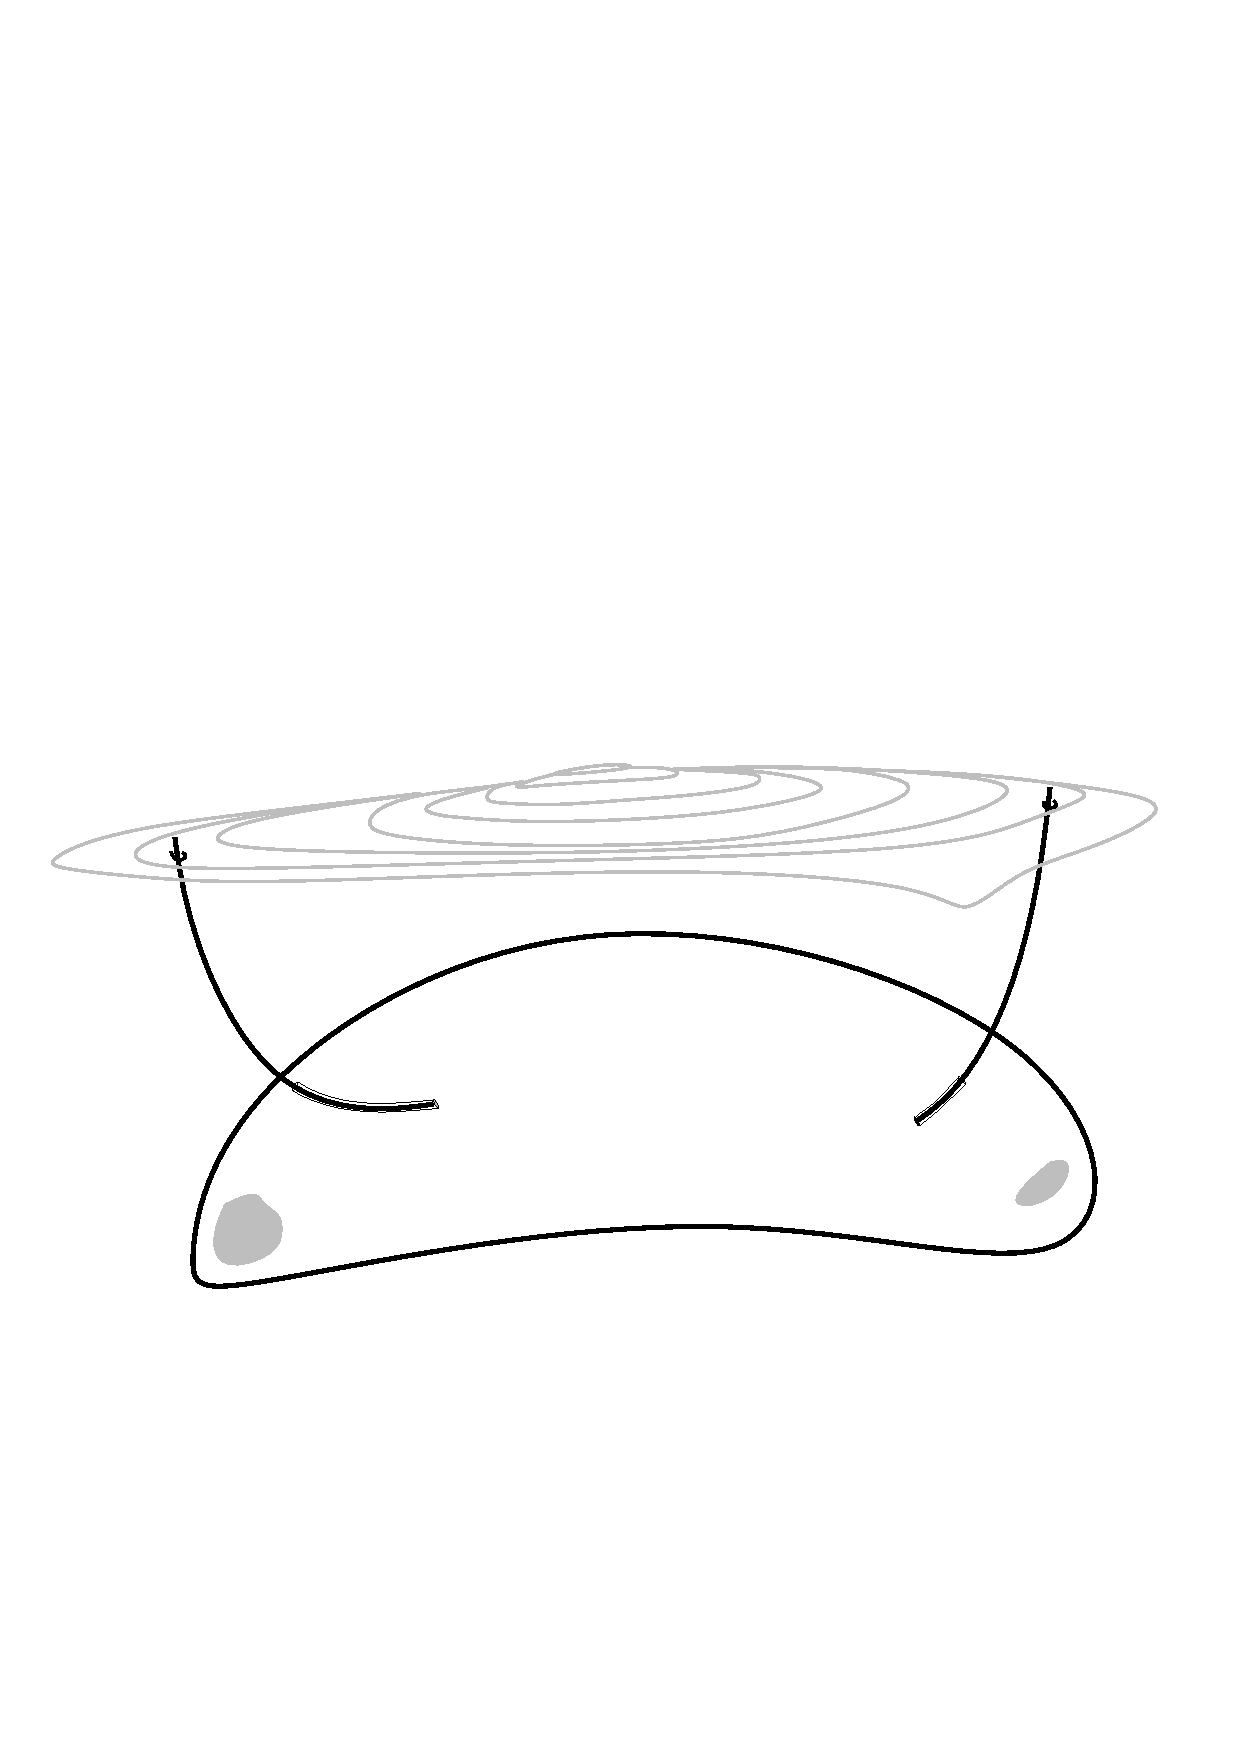
\includegraphics[scale=0.8]{Fig/yacimiento.pdf}%
	\caption[Esquemático de un yacimiento cerrado.]{Esquemático de un yacimiento cerrado. Los autores.}
	\label{fig:empanada}
\end{figure}

Además para un tiempo $t=0$ se tiene que:
\begin{align}
	P_{f}(\vec{x},0) = P^{0}_{f}(\vec{x}) \qquad \forall f \in \left\lbrace o,g,w\right\rbrace\\
	S_{f}(\vec{x},0) = S^{0}_{f}(\vec{x}) \qquad \forall f \in \left\lbrace o,g,w\right\rbrace
\end{align}
%
Es decir, existe funciones en el espacio que describen las condiciones iniciales de presión $P^{0}_{f}(\vec{x})$ y saturación $S^{0}_{f}(\vec{x})$ para los fluidos $f$ del yacimiento.

\subsection{Discretización}\label{subsec:Discretization}

Se elige el método de los volúmenes finitos para las discretización espacial de las ecuaciones \ref{ec:aceite}, \ref{ec:gas} y \ref{ec:agua} y un esquema implícito para la discretización del tiempo, es decir, elección del tiempo al $n+1$ (futuro). El proceso de discretización se muestra en el anexo \ref{AnexoA}. Para una celda con índice $i$ con superficie $S$ como un conjunto de caras $c$, la discretización de las ecuaciones es la siguiente:
%Algebraic Equations
\begin{align}
\label{ec:aceiteDiscretizacion}&\underbrace{\frac{|\Omega_{i}|}{\Delta t}\left[ \phi_{i} \left( \frac{S_{o,i}}{B_{o,i}} + \frac{R_{v,i}S_{g,i}}{B_{g,i}}\right)\right]^{n+1}_{n}}_{\text{Acumulación - Aceite}} + 
\underbrace{\sum_{c \in S}\left[ T^{n+1}_{o,c} \nabla{\Phi_{o,c}^{n+1}} + R_{v,c}T^{n+1}_{g,c} \nabla{\Phi_{g,c}^{n+1}} \right] }_{\text{Flujo - Aceite}}+ \dot{Q}_{o,i}^{n+1} = 0 \\
\label{ec:gasDiscretizacion}&\underbrace{\frac{|\Omega_{i}|}{\Delta t}\left[ \phi_{i} \left( \frac{S_{g,i}}{B_{g,i}} + \frac{R_{s,i}S_{o,i}}{B_{o,i}}\right)\right]^{n+1}_{n}}_{\text{Acumulación - Gas}} + 
\underbrace{\sum_{c \in S}\left[ T^{n+1}_{g,c}\nabla{\Phi_{g,c}^{n+1} + R_{s,c}T^{n+1}_{o,c} \nabla{\Phi_{o,c}^{n+1}}} \right] }_{\text{Flujo - Gas}}+ Q_{g,i}^{n+1} = 0 \\
\label{ec:aguaDiscretizacion}&\underbrace{\frac{|\Omega_{i}|}{\Delta t}\left[ \phi_{i} \left( \frac{S_{w,i}}{B_{w,i}}\right)\right]^{n+1}_{n}}_{\text{Acumulación - Agua}}
+ 
\underbrace{\sum_{c \in S}\left[ T^{n+1}_{w,c}\nabla{\Phi_{w,c}^{n+1}} \right]}_{\text{Flujo - Agua}} + Q_{w,i}^{n+1} = 0 
\end{align}\\

dónde:

\begin{align*}
	&\left[ \phi_{i} \left( \frac{S_{o,i}}{B_{o,i}} + \frac{R_{v,i}S_{g,i}}{B_{g,i}}\right)\right]^{n+1}_{n} = 
	\phi^{n+1}_{i} \left( \frac{S_{o,i}^{n+1}}{B_{o,i}^{n+1}} + \frac{R_{v,i}^{n+1}S_{g,i}^{n+1}}{B_{g,i}^{n+1}}\right) - \phi^{n}_{i} \left( \frac{S_{o,i}^{n}}{B_{o,i}^{n}} + \frac{R_{v,i}^{n}S_{g,i}^{n}}{B_{g,i}^{n}}\right),\\
	&\left[ \phi_{i} \left( \frac{S_{g,i}}{B_{g,i}} + \frac{R_{s,i}S_{o,i}}{B_{o,i}}\right)\right]^{n+1}_{n} = 
	\phi^{n+1}_{i} \left( \frac{S_{g,i}^{n+1}}{B_{g,i}^{n+1}} + \frac{R_{s,i}^{n+1}S_{o,i}^{n+1}}{B_{o,i}^{n+1}}\right) - \phi^{n}_{i} \left( \frac{S_{g,i}^{n}}{B_{g,i}^{n}} + \frac{R_{s,i}^{n}S_{o,i}^{n}}{B_{o,i}^{n}}\right),\\
	&\left[ \phi_{i} \left( \frac{S_{w,i}}{B_{w,i}}\right)\right]^{n+1}_{n} = 
	\phi^{n+1}_{i} \left( \frac{S_{w,i}^{n+1}}{B_{w,i}^{n+1}}\right) - \phi^{n}_{i} \left( \frac{S_{w,i}^{n}}{B_{w,i}^{n}}\right)
\end{align*}

El término $T_{f,c}$ en la Ecuación \ref{ec:Transmissibity} corresponde a la transmisividad en una cara $c$ que conecta una celda $i$ con otra celda $j$.

\begin{align}
	\label{ec:Transmissibity}& T_{f,c} = \left(\frac{1}{(\Delta l_{i}/A_{c}K_{l,i})+(\Delta l_{j}/A_{c}K_{l,j})}\right)\frac{k_{rf,c}}{\mu_{f,c}B_{f,c}}
\end{align}
\subsection{Modelado de Pozos}
%
Los pozos son el principal objeto de estudio de la simulación de yacimientos de petróleo, debido a que en ellos, se concentra el propósito de cualquier operación de campo. Los pozos tienen dos tipos, inyector o productor, y se forman por un conjunto de bloques perforados en los que existe un flujo radial \citep{peaceman1983interpretation}. \cite{peaceman1983interpretation} describe el flujo en pozos con varias capas de perforados como se muestra en la Ecuación \ref{ec:peaceman}. En la Figura \ref{fig:mulperfwell} se ilustra un pozo vertical con múltiples perforados.

\begin{figure}[h]
	\centering%
	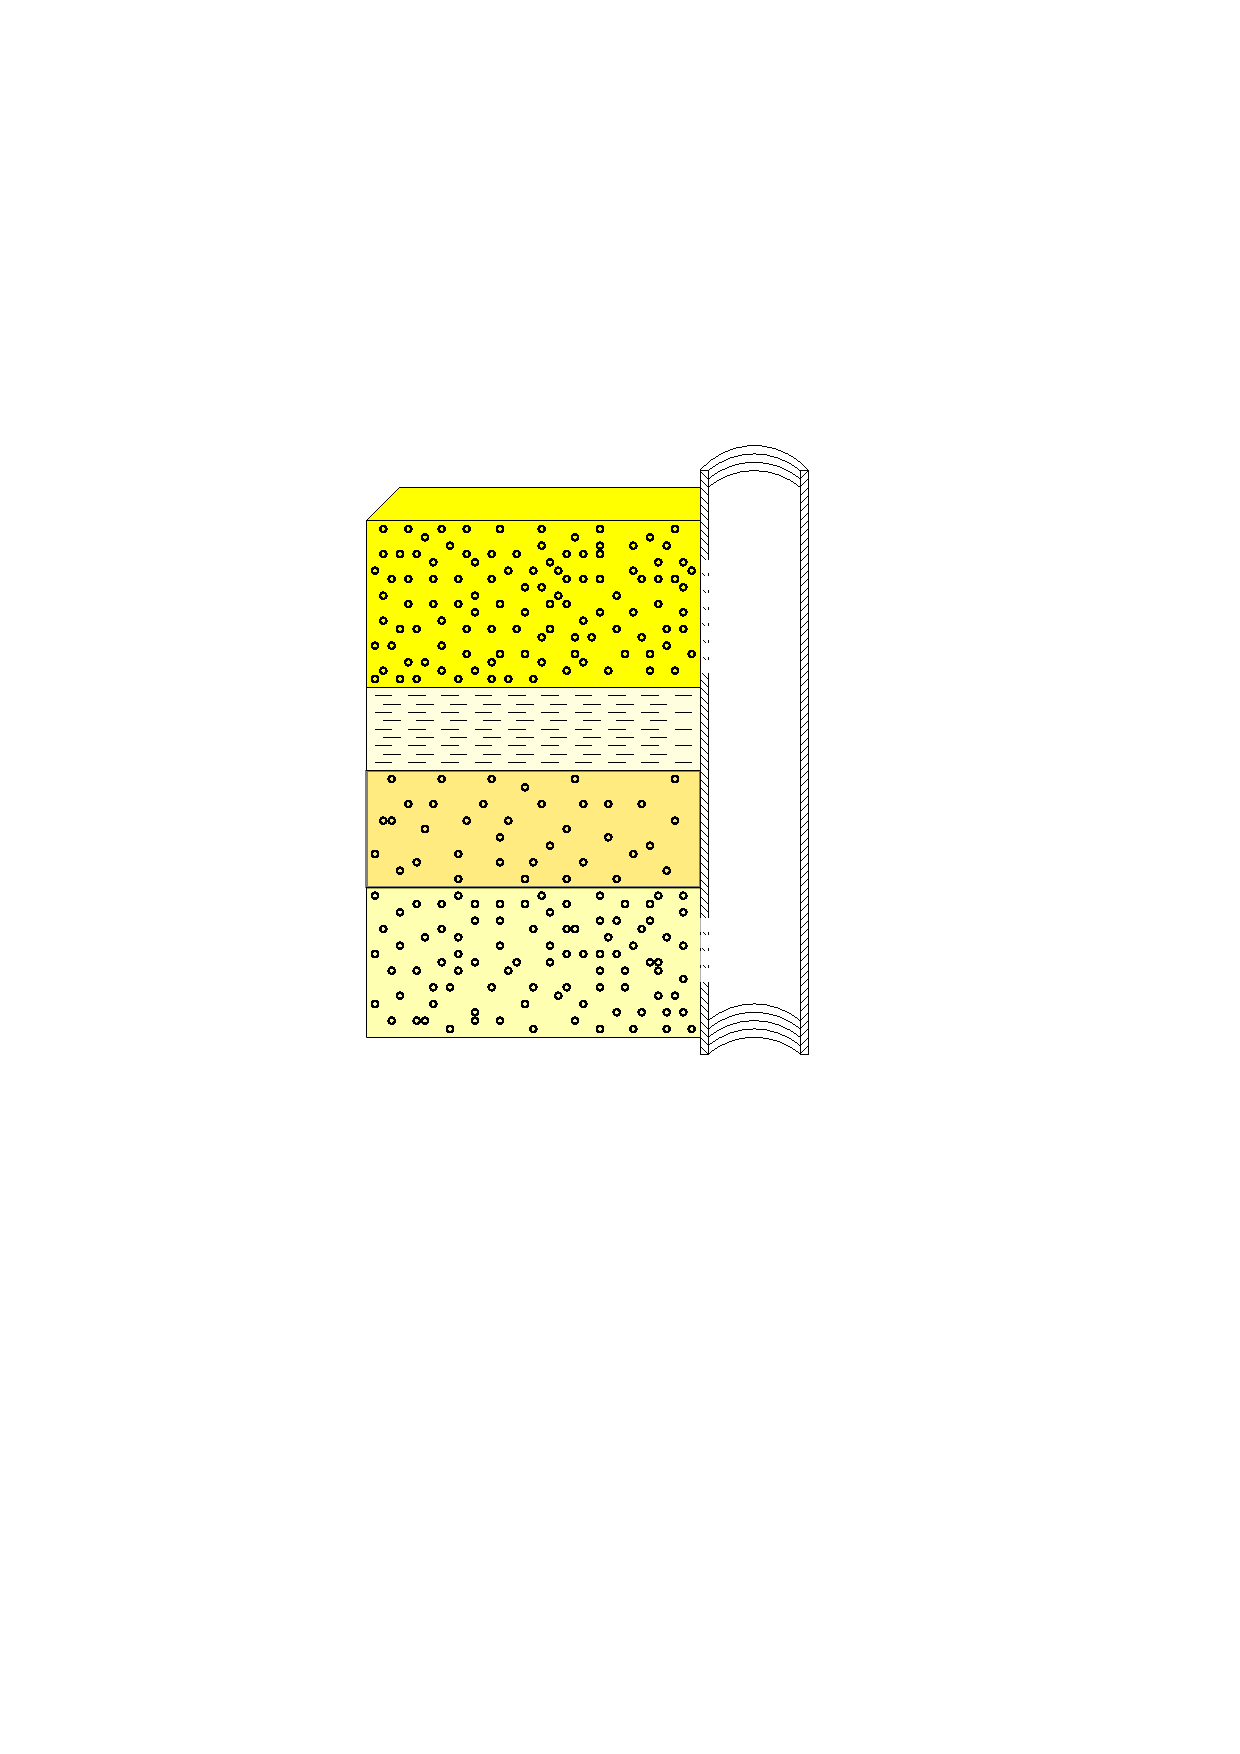
\includegraphics[scale=0.8]{Fig/pozo_multi_perf.pdf}%
	\caption[Esquemático de pozo multiperforado.]{Esquemático de pozo multiperforado. Elaboración a partir de \cite{chen2007reservoir}} \label{fig:mulperfwell}
\end{figure}

\begin{align}
	\label{ec:peaceman}&q^{(v)}_{f} = \sum_{m=1}^{M^{(v)}_{w}}\frac{2\pi k_{rf} \rho_{f} \sqrt{k_{xx}k_{yy}}h_{z}}{\mu_{f}\left(\ln \left(r_{e}/r_{w}\right) +s\right)}\left(p_{bh}^{(v)}-p_{f,m}-\gamma\left(z_{bh}^{(v)}-z_{m}\right)\right)\delta\left(x-x_{m}^{(v)}\right)
\end{align}
%
{\color{red} No he hablado de condiciones operativas}

\subsection{Método de Newton-Raphson}\label{subsec:N-R}
%
El sistema de ecuaciones algebraicas que se forman por \ref{ec:aceiteDiscretizacion}, \ref{ec:gasDiscretizacion} y \ref{ec:aguaDiscretizacion} es no lineal, por lo tanto, se aplica el método del Newton-Raphson el cuál se usa para encontrar las raíces de una ecuación no lineal aproximando su derivada, como se ilustra en la Figura \ref{fig:NewtonR}.\\

\begin{figure}[h]
	\centering%
	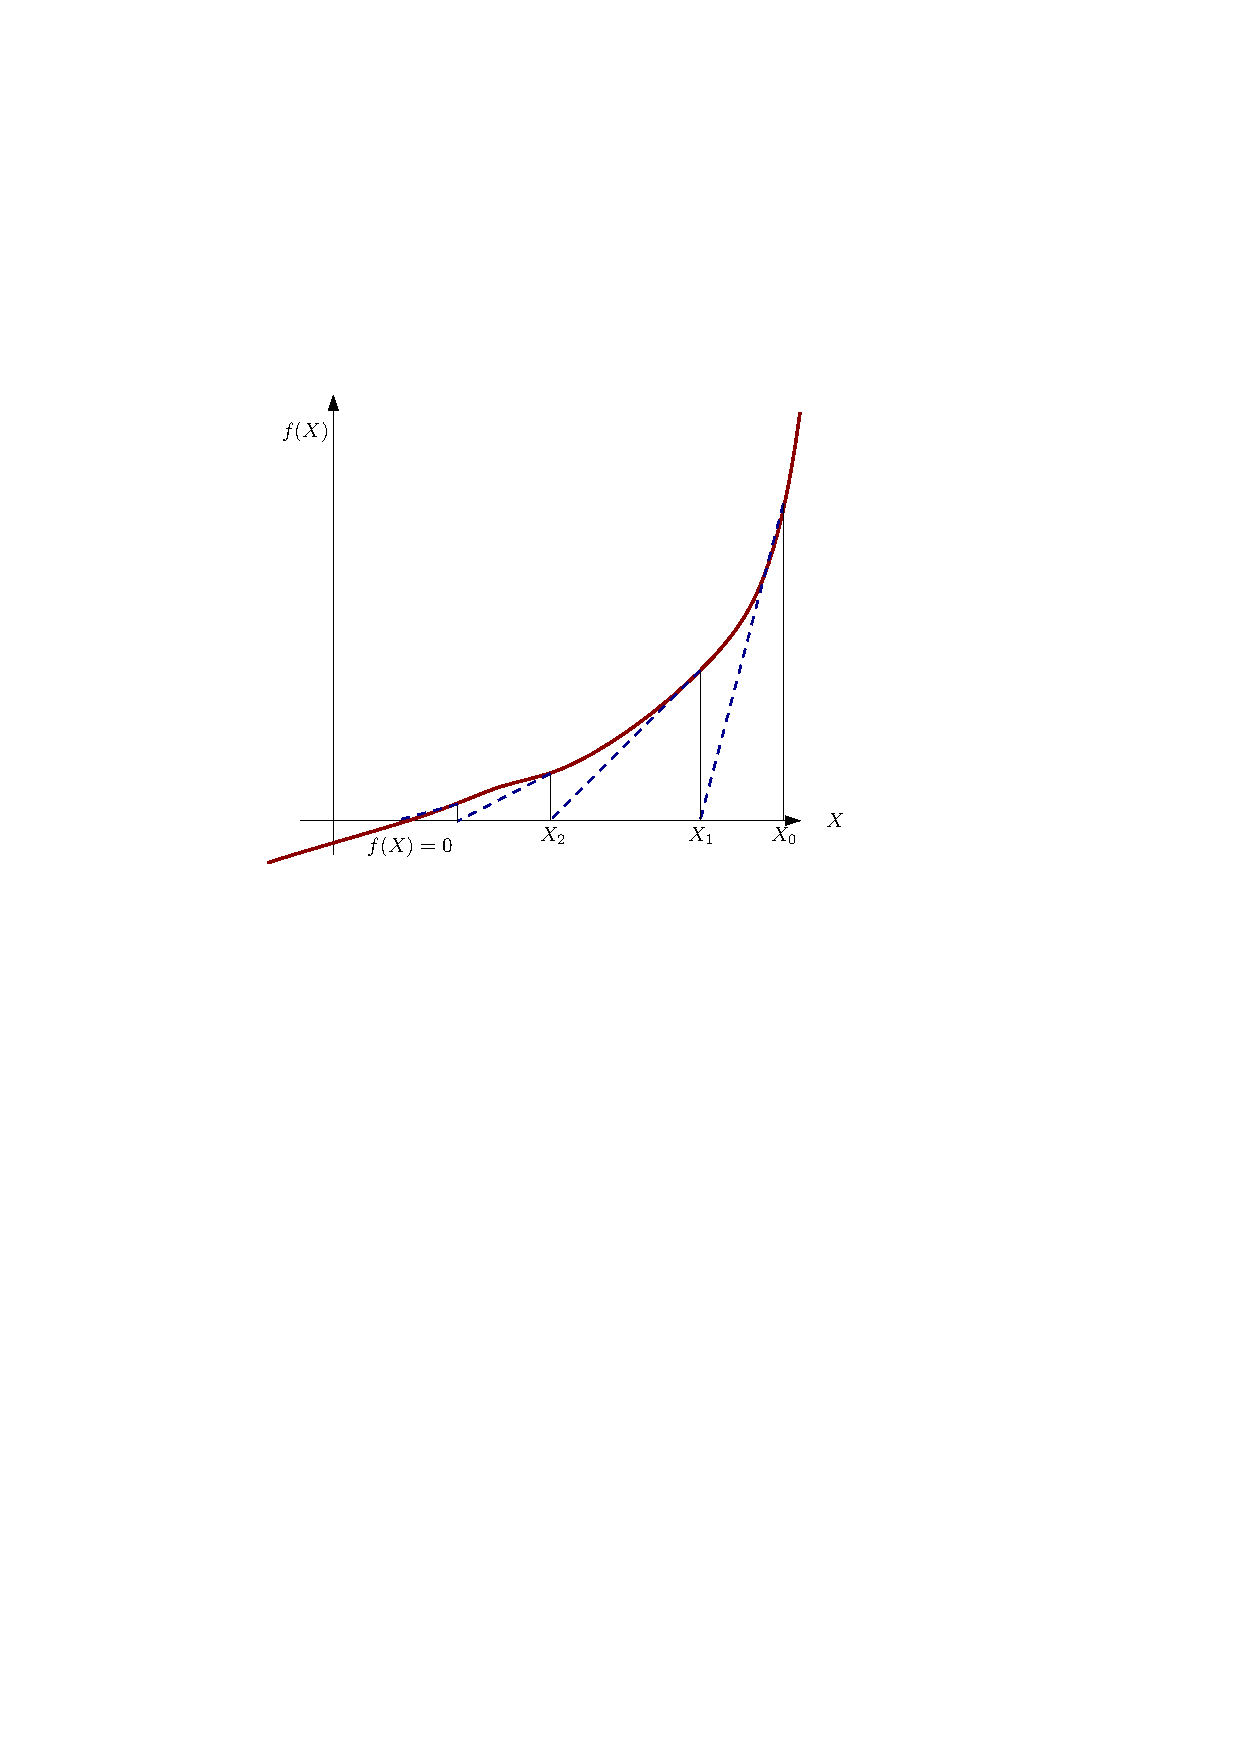
\includegraphics[scale=0.8]{Fig/NewtonR.pdf}%
	\caption[Aproximación a la derivada de una función.]{Aproximación a la derivada de una función. {\color{red} Elaboración a partir de .}} \label{fig:NewtonR}
\end{figure}
~\\
\begin{equation}
A \cdot {\Delta \vec{x}} = \vec{b} \Leftrightarrow J^{k}_{i,j} \cdot {\Delta \vec{x}} = -\vec{R^{k}_{i}}
\end{equation}
\begin{equation}
\Delta \vec{x} = \vec{x}^{k+1} - \vec{x}^{k} = \left(\Delta P_o, \Delta S_g, \Delta S_w \right)^T
\end{equation}
\begin{equation}
-\vec{R^k_i} = \left(\Delta R^k_{P_o,i}, \Delta R^k_{S_g,i}, \Delta R^k_{S_w,i} \right)^T
\end{equation}
\begin{equation}
J^k_{i,j}=\frac{\partial R^k_i}{\partial x^k_j}	
\end{equation}
\begin{equation}
\frac{\partial R^k}{\partial x^k} \approx \frac{R\left(x^k + \xi \right) - R\left(x^k \right)}{\xi}
\end{equation}

\section{Procesos de Recobro Mejorado}\label{sec:EOR}

\subsection{Modelado del Químico}\label{subsec:Chemical}

%\section{Procesos de Recobro Mejorado}

\section{Esquemas Preconceptuales}\label{sec:EP}

Los Esquemas Preconceptuales (EP) son representaciones intermedias entre el lenguaje natural y un esquema conceptual o un lenguaje formal. Estos esquemas contienen todo el dominio de aplicación de un interesado y, por tanto, sirven para establecer un punto común de entendimiento entre un interesado y un analista de software \citep{zapata2007phd}. Los EP se desarrollan con la idea de mantener la coherencia y consistencia entre el discurso del interesado y el software que se desarrolla. 

\subsection{Elementos del Esquema Preconceptual}\label{subsec:ElementsEP}
\cite{zapata2012unc} define los elementos del EP tal como se observa en la Figura \ref{fig:InitialPS} para la representación del dominio del interesado. Estos elementos se dividen en cuatro categorías: nodos, relaciones, enlaces, y aglutinadores.\\

\begin{figure}[h]
	\centering%
	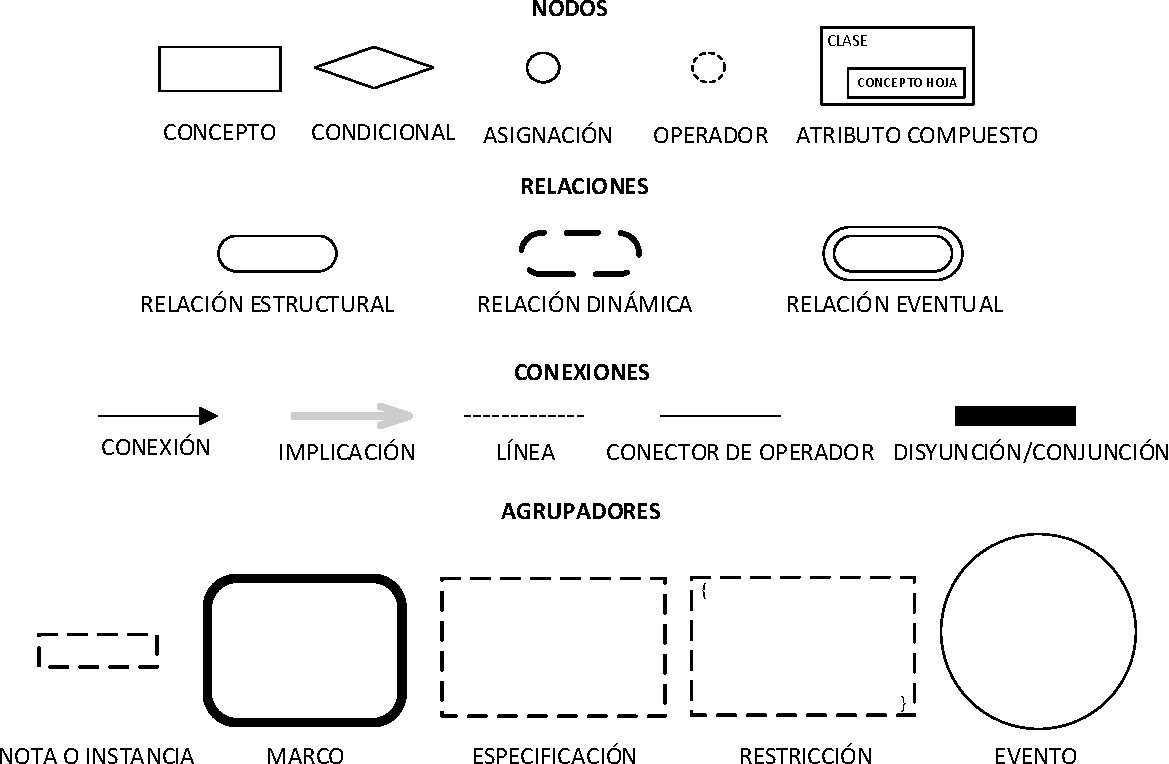
\includegraphics[scale=0.51]{Fig/ElementosDelEP.pdf}%
	\caption[Elementos del EP.]{Elementos del EP. \citep{zapata2012unc}.} \label{fig:InitialPS}
\end{figure}

\subsubsection{Nodos}
\begin{itemize}
	\item \textbf{Concepto}:
	sustantivo o sintagma nominal que representa un actor u objeto dentro del dominio del interesado. Se subclasifican en conceptos clase y conceptos hoja, según su jerarquía \citep{zapata2007phd,zapata2012unc}. %En la figura \ref{fig:PS_Concept} se muestra la representación. Un ejemplo de su uso se presenta en la figura \ref{fig:ej_concept}.
	
	\item \textbf{Condicional}: condición para ejecutar una relación dinámica o una especificación a partir de una expresión lógica formada por conceptos o variables, operadores, y valores o parámetros \citep{zapata2007phd,zapata2012unc}. %como se muestra en la figura \ref{fig:}
	
	\item \textbf{Operador}: símbolo lógico o matemático que sirve para formar expresiones a evaluar \citep{zapata2012unc}.
	
	\item \textbf{Asignación}: Sirve para asignar el valor que resulta de una expresión matemática o lógica \citep{zapata2012unc}.
	
	\item \textbf{Concepto Clase}: Sirve para representar el acceso a un concepto hoja o atributo desde su concepto contenedor \citep{zapata2007phd}.
\end{itemize}

\subsubsection{Relaciones}
\begin{itemize}
	\item \textbf{Relación Estructural}: Relación permanente entre dos conceptos. Se asocia con los verbos ``ser'' o ``tener'', y que significan generalización o agregación, respectivamente \citep{zapata2007phd,zapata2012unc}.
	\item \textbf{Relación Dinámica}: Se asocia con verbos que denotan acción u operaciones que modifican el dominio de estudio; permite establecer relaciones transitorias entre el concepto ejecutor de la acción y el concepto objeto de dicha acción \citep{zapata2007phd,zapata2012unc}.
	\item \textbf{Relación Eventual}: Se relaciona con un verbo que denota ocurrencia, el cuál no se asocia a un concepto ejecutor. \citep{zapata2012unc,norena2018Ling}.
\end{itemize}

\subsubsection{Enlaces}
\begin{itemize}
	\item \textbf{Conexión}: Es una flecha unidireccional que sirve para conectar conceptos con relaciones dinámicas o estructurales \citep{zapata2007phd,zapata2012unc}.
	\item \textbf{Implicación}: Es una línea continua y dirigida que sirve para indicar una relación causa-efecto u orden entre relaciones dinámicas, condicionales o eventos. \citep{zapata2007phd,zapata2012unc}. 
	\item \textbf{Concepto-Nota}: Sirve para conectar un concepto a una nota o instancia \citep{zapata2007phd,zapata2012unc}.
	\item \textbf{Conector de Operador}: Sirve para conectar un valor, concepto, atributo compuesto u otros operadores, a un operador \citep{zapata2012unc}. 
	\item \textbf{Conjunción/Disyunción}: Sirve para agrupar o bifurcar implicaciones, estableciendo una causalidad conjunta o múltiples efectos \citep{zapata2007phd,zapata2012unc}. 
\end{itemize}

\subsubsection{Aglutinadores}
\begin{itemize}
	\item \textbf{Nota o Instancia}: Sirve para limitar los valores para un concepto a un conjunto predefinido \citep{zapata2007phd,zapata2012unc}.
	\item \textbf{Especificación}: Sirve para agrupar un conjunto de operaciones que describen una relación dinámica o eventual \citep{zapata2012unc}.
	\item \textbf{Marco}: Sirve para asociar múltiples relaciones dinámicas a una responsabilidad o para agrupar conceptos \citep{zapata2012unc}.
	\item \textbf{Restricción}: Sirve para establecer una condición sobre una especificación de operaciones \citep{zapata2012unc}. Adicionalmente, se usa para establecer ciclos sobre conceptos o condiciones \citep{JChaverra}.
	\item \textbf{Evento}: Es una ocurrencia que habilita cambios de estado en los procesos  \citep{zapata2013Eventos}.
\end{itemize}

\subsection{Esquemas Preconceptuales en el contexto del software científico}\label{subsec:EPScientific}

\cite{JCalle} y \cite{norena2018det} descubren la capacidad del EP para representar aplicaciones en el contexto del software científico. Para ello, definen elementos adicionales que permiten modelar dominios de mayor complejidad. En esta Tesis de Maestría se usan las condiciones iniciales, conceptos tipo arreglo, parámetros, variables, vectores, operadores predefinidos, operador ``\textit{push}'', operador ``\textit{type}'',  y funciones que define el analista. En la Figura \ref{fig:NewElements} se representan los elementos previamente mencionados. A continuación, se explican los elementos adicionales que se usan en el desarrollo de esta Tesis de Maestría.

\begin{figure}[h]
	\centering%
	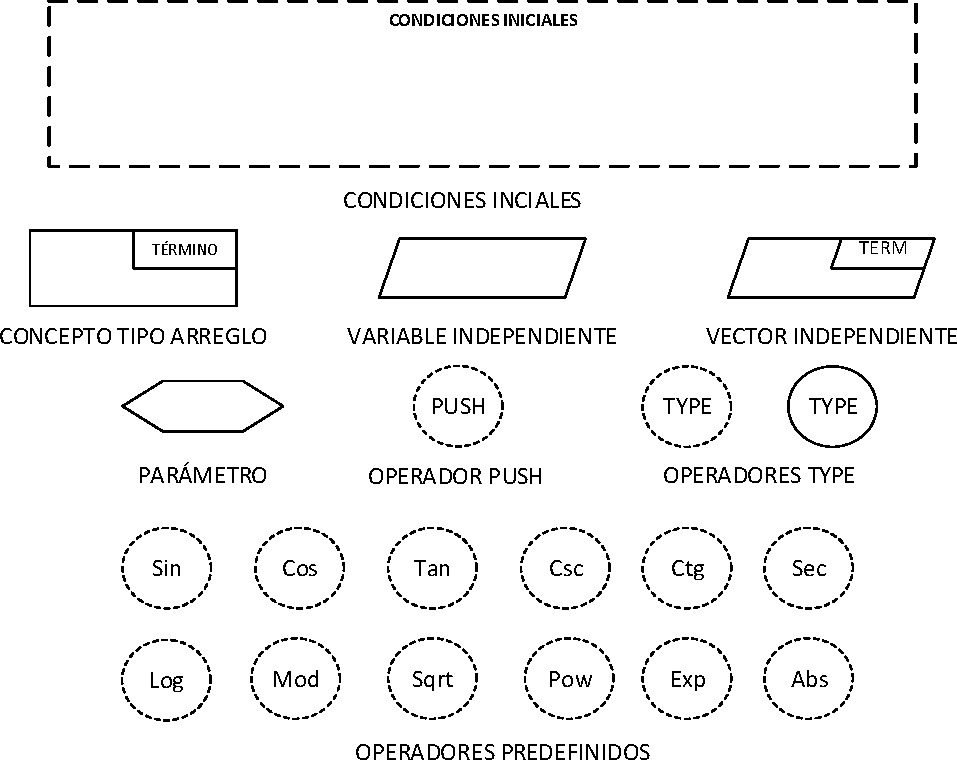
\includegraphics[width=0.9\linewidth]{Fig/NuevosElementosDelEP.pdf}%
	\caption[Elementos para la representación de Software Científico.]{Elementos para la representación de Software Científico. \citep{JCalle,norena2018det}.} \label{fig:NewElements}
\end{figure}

\subsubsection{Condiciones Iniciales}
Las condiciones iniciales son especificaciones, de variables y parámetros globales, que se conoce desde el inicio de la simulación \citep{norena2018det}. Un ejemplo de uso se presenta en la Figura \ref{fig:EjInitialConditions}.

\begin{figure}[h]
	\centering%
	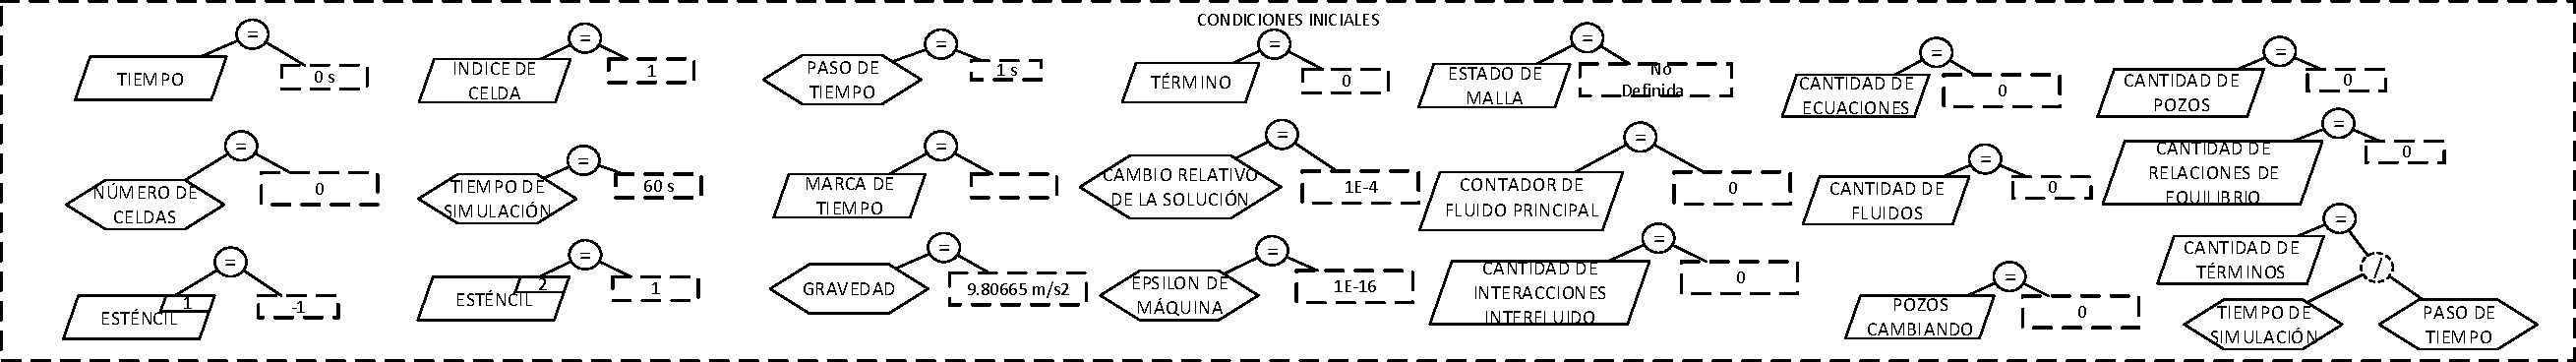
\includegraphics[width=0.9\linewidth]{Fig/EjInitialConditions.pdf}%
	\caption[Ejemplo de Condiciones Iniciales.]{Ejemplo de Condiciones Iniciales. Los autores.} \label{fig:EjInitialConditions}
\end{figure}

\subsubsection{Concepto tipo arreglo}
Los conceptos tipo arreglo permiten almacenar de manera permanente múltiples valores, y a su vez, iterar sobre ellos \citep{JCalle}. En esta Tesis de Maestría se usan conceptos tipo arreglos multidimensionales. En la Figura \ref{fig:EjArrConcept} se expone un ejemplo de su uso.

\begin{figure}[h]
	\centering%
	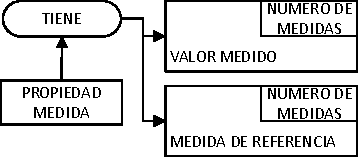
\includegraphics[scale=1]{Fig/EjArrConcepts.pdf}%
	\caption[Ejemplo de Conceptos tipo arreglo.]{Ejemplo de Conceptos tipo arreglo. Los autores.} \label{fig:EjArrConcept}
\end{figure}

\subsubsection{Parámetro}
Los parámetros se usan para almacenar constantes o definir entradas en la especificación de relaciones dinámicas, especificaciones de tipo marco y funciones, que reciben múltiples argumentos o parámetros \citep{JCalle, norena2018det}. Se expone un ejemplo de uso en la Figura \ref{fig:EjParameter}.\\

\begin{figure}[h]
	\centering%
	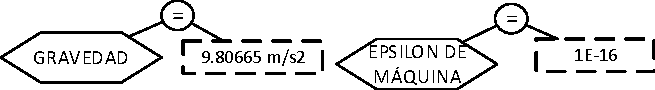
\includegraphics[width=0.5\linewidth]{Fig/EjParametro.pdf}%
	\caption[Ejemplo de parámetros.]{Ejemplo de parámetros. Los autores.} \label{fig:EjParameter}
\end{figure}

\subsubsection{Variable Independiente}
Las variables independientes permiten almacenar valores durante la ejecución de una especificación sin estar acopladas a un concepto. Si se definen en las condiciones iniciales, se pueden usan de manera global durante toda la simulación \citep{norena2018det}. En la Figura \ref{fig:EjInitialConditions} se pueden ver ejemplos de variables independientes.\\

\subsubsection{Vector independiente}
Los vectores independientes cumplen la misma tarea y propiedades de las variables independientes, pero permiten almacenar más de un valor \citep{norena2018det}. Un ejemplo de vector independiente se presenta en la Figura \ref{fig:EjVector}.

\begin{figure}[h]
	\centering%
	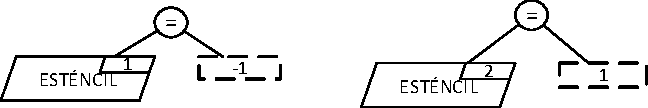
\includegraphics[width=0.5\linewidth]{Fig/EjVectorIndependiente.pdf}%
	\caption[Ejemplo de vector independiente.]{Ejemplo de vector independiente. Los autores.} \label{fig:EjVector}
\end{figure}

\subsubsection{Operadores Predefinidos}
Son funciones algebraicas y trigonométricas predefinidas que se pueden usar como operadores en el EP \citep{JCalle}.

\subsubsection[Operador \emph{Push}]{Operador {\normalfont \bfseries \itshape Push}}
El operador \textit{Push} sirve para insertar, valores, conceptos o parámetros dentro de un concepto tipo arreglo, el elemento que se inserta queda en la última posición del arreglo  \citep{JCalle}.
\subsubsection[Operador \emph{Type}]{Operador {\normalfont \bfseries \itshape Type}}
El operador \textit{Type} tiene dos versiones: una como operador de asignación y otra como operador de información. En el caso de la asignación, sirve para otorgarle el tipo de una subclase a un concepto. Mientras que en el de información, permite consultar si el tipo del concepto corresponde con el tipo de una subclase definida \citep{JCalle}.
\subsubsection{Funciones que define el analista}
Las funciones que define el analista son especificaciones reutilizables en el EP a modo de un operador personalizado cuyo nombre define el analista. Estas funciones llevan en su especificación un concepto ``\textit{return}'' que corresponde al valor que devuelve la función cuando se usa como operador \citep{JCalle}. En la figura \ref{fig:Potencial} se presenta un ejemplo de definición y uso de una función que define el analista.

\begin{figure}[h]
	\centering%
	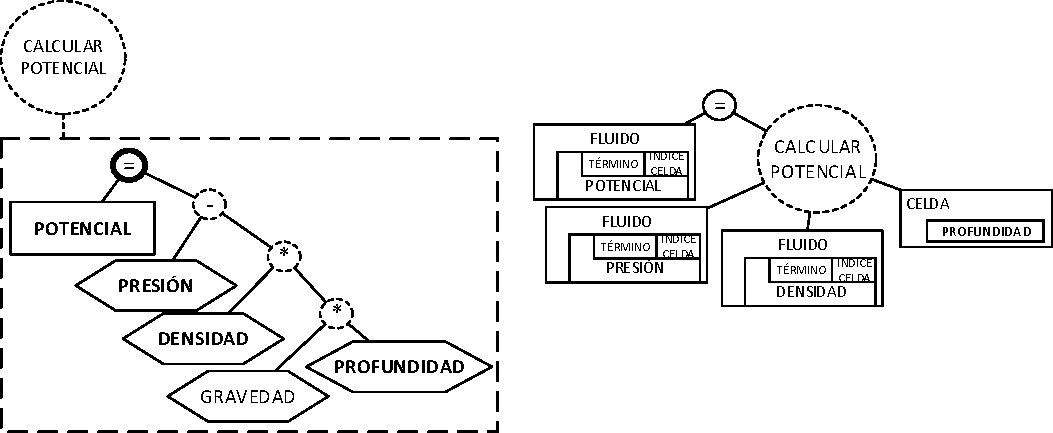
\includegraphics[scale=0.8]{Fig/EjFuncion.pdf}%
	\caption[Ejemplo de función, cálculo del potencial.]{Ejemplo de función, cálculo del potencial. Los autores.} \label{fig:Potencial}
\end{figure}

\section{Modelo Ejecutable}\label{sec:Executable}
Un modelo ejecutable es una abstracción que permite describir y definir la conceptualización y comportamiento de un dominio real o hipotético de estudio. Además, cuentan con semánticas que permiten definir acciones \citep{ExecutableUML}. El EP se enmarca dentro de esta definición, puesto que los EP ejecutables tienen elementos que permiten representar acciones que se procesan internamente en el modelo \citep{JChaverra}. 
%\chapter{Cap\'{\i}tulo 2}
%Existen varias normas para la citaci\'{o}n bibliogr\'{a}fica. Algunas \'{a}reas del conocimiento prefieren normas espec\'{\i}ficas para citar las referencias bibliogr\'{a}ficas en el texto y escribir la lista de bibliograf\'{\i}a al final de los documentos. Esta plantilla brinda la libertad para que el autor de la tesis  o trabajo de investigaci\'{o}n utilice la norma bibliogr\'{a}fica com\'{u}n para su disciplina. Sin embargo, se solicita que la norma seleccionada se utilice con rigurosidad, sin olvidar referenciar "todos" los elementos tomados de otras fuentes (referencias bibliogr\'{a}ficas, patentes consultadas, software empleado en el manuscrito, en el tratamiento a los datos y resultados del trabajo, consultas a personas (expertos o p\'{u}blico general), entre otros).\\
%
%\section{Ejemplos de citaciones bibliogr\'{a}ficas}
%Existen algunos ejemplos para la citaci\'{o}n bibliogr\'{a}fica, por ejemplo, Microsoft Word (versiones posteriores al 2006), en el  men\'{u} de referencias, se cuenta con la opci\'{o}n de insertar citas bibliogr\'{a}ficas utilizando la norma APA (American Psychological Association) u otras normas y con la ayuda para construir autom\'{a}ticamente la lista al final del documento. De la misma manera, existen administradores bibliogr\'{a}ficos compatibles con Microsoft Word como Zotero, End Note y el Reference Manager,  disponibles a trav\'{e}s del Sistema Nacional de Bibliotecas (SINAB) de la Universidad Nacional de Colombia\footnote{Ver:www.sinab.unal.edu.co } secci\'{o}n "Recursos bibliogr\'{a}ficos" opci\'{o}n "Herramientas Bibliogr\'{a}ficas. A continuaci\'{o}n se muestra un ejemplo de una de las formas m\'{a}s usadas para las citaciones bibliogr\'{a}ficas.\\
%
%Citaci\'{o}n individual:\cite{AG01}.\\
%Citaci\'{o}n simult\'{a}nea de varios autores:
%\cite{AG12,AG52,AG70,AG08a,AG09a,AG36a,AG01i}.\\
%
%Por lo general, las referencias bibliogr\'{a}ficas correspondientes a los anteriores n\'{u}meros, se listan al final del documento en orden de aparici\'{o}n o en orden alfab\'{e}tico. Otras normas de citaci\'{o}n incluyen el apellido del autor y el a\~{n}o de la referencia, por ejemplo: 1) "...\'{e}nfasis en elementos ligados al \'{a}mbito ingenieril que se enfocan en el manejo de datos e informaci\'{o}n estructurada y que seg\'{u}n Kostoff (1997) ha atra\'{\i}do la atenci\'{o}n de investigadores dado el advenimiento de TIC...", 2) "...Dicha afirmaci\'{o}n coincide con los planteamientos de Snarch (1998), citado por Castellanos (2007), quien comenta que el manejo..." y 3) "...el futuro del sistema para argumentar los procesos de toma de decisiones y el desarrollo de ideas innovadoras (Nosella \textsl{et al}., 2008)...".\\
%
%\section{Ejemplos de presentaci\'{o}n y citaci\'{o}n de figuras}
%Las ilustraciones forman parte del contenido de los cap\'{\i}tulos. Se deben colocar en la misma p\'{a}gina en que se mencionan o en la siguiente (deben siempre mencionarse en el texto).\\
%
%Las llamadas para explicar alg\'{u}n aspecto de la informaci\'{o}n deben hacerse con nota al pie y su nota correspondiente\footnote{Las notas van como "notas al pie". Se utilizan para explicar, comentar o hacer referencia al texto de un documento, as\'{\i} como para introducir comentarios detallados y en ocasiones para citar fuentes de informaci\'{o}n (aunque para esta opci\'{o}n es mejor seguir en detalle las normas de citaci\'{o}n bibliogr\'{a}fica seleccionadas).}. La fuente documental se debe escribir al final de la ilustraci\'{o}n o figura con los elementos de la referencia (de acuerdo con las normas seleccionadas) y no como pie de p\'{a}gina. Un ejemplo para la presentaci\'{o}n y citaci\'{o}n de figuras, se presenta a continuaci\'{o}n (citaci\'{o}n directa):\\
%
%Por medio de las propiedades del fruto, seg\'{u}n el espesor del endocarpio, se hace una clasificaci\'{o}n de la palma de aceite en tres tipos: Dura, Ternera y Pisifera, que se ilustran en la Figura
%\ref{fig:Fruto}.\\
%\begin{figure}[h]
%\centering%
%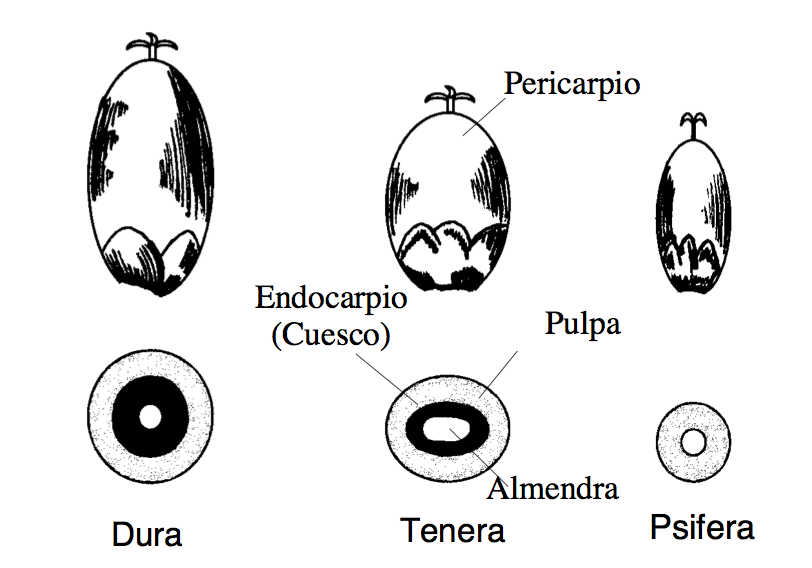
\includegraphics{Kap3/FrutoSp}%
%\caption{Tipos y partes del fruto de palma de aceite \cite{AG03p,AG04p}.} \label{fig:Fruto}
%\end{figure}
%
%\section{Ejemplo de presentaci\'{o}n y citaci\'{o}n de tablas y cuadros}
%Para la edici\'{o}n de tablas, cada columna debe llevar su t\'{\i}tulo; la primera palabra se debe escribir con may\'{u}scula inicial y preferiblemente sin abreviaturas. En las tablas y cuadros, los t\'{\i}tulos y datos se deben ubicar entre l\'{\i}neas horizontales y verticales cerradas (como se realiza en esta plantilla).\\
%
%La numeraci\'{o}n de las tablas se realiza de la misma manera que las figuras o ilustraciones, a lo largo de todo el texto. Deben llevar un t\'{\i}tulo breve, que concreta el contenido de la tabla; \'{e}ste se debe escribir en la parte superior de la misma. Para la presentaci\'{o}n de cuadros, se deben seguir las indicaciones dadas para las tablas.\\
%
%Un ejemplo para la presentaci\'{o}n y citaci\'{o}n de tablas (citaci\'{o}n indirecta), se presenta a continuaci\'{o}n:\\
%
%De esta participaci\'{o}n aproximadamente el 60 \% proviene de biomasa
%(Tabla \ref{EMundo1}).
%\begin{center}
%\begin{threeparttable}
%\centering%
%\caption{Participaci\'{o}n de las energ\'{\i}as renovables en el suministro
%total de energ\'{\i}a primaria \cite{AG02i}.}\label{EMundo1}
%\begin{tabular}{|l|c|c|}\hline
%&\multicolumn{2}{c|}{Participaci\'{o}n en el suministro de energ\'{\i}a primaria /\% (Mtoe)\;$\tnote{1}$}\\\cline{2-3}%
%\arr{Region}&Energ\'{\i}as renovables &Participaci\'{o}n de la biomasa\\\hline%
%Latinoam\'{e}rica&28,9 (140)&62,4 (87,4)\\\hline%
%\:Colombia&27,7 (7,6)&54,4 (4,1)\\\hline%
%Alemania&3,8 (13,2)&65,8 (8,7)\\\hline%
%Mundial&13,1 (1404,0)&79,4 (1114,8)\\\hline
%\end{tabular}
%\begin{tablenotes}
%\item[1] \footnotesize{1 kg oe=10000 kcal=41,868 MJ}
%\end{tablenotes}
%\end{threeparttable}
%\end{center}
%
%NOTA: en el caso en que el contenido de la tabla o cuadro sea muy extenso, se puede cambiar el tama\~{n}o de la letra, siempre y cuando \'{e}sta sea visible por el lector.\\
%
%\subsection{Consideraciones adicionales para el manejo de figuras y tablas}
%Cuando una tabla, cuadro o figura ocupa m\'{a}s de una p\'{a}gina, se debe repetir su identificaci\'{o}n num\'{e}rica, seguida por la palabra continuaci\'{o}n.\\
%
%Adicionalmente los encabezados de las columnas se deben repetir en todas las p\'{a}ginas despu\'{e}s de la primera.\\
%
%Los anteriores lineamientos se contemplan en la presente plantilla.\\
%
%\begin{itemize}
%\item Presentaci\'{o}n y citaci\'{o}n de ecuaciones.
%\end{itemize}

%La citaci\'{o}n de ecuaciones, en caso que se presenten, debe hacerse como lo sugiere esta plantilla. Todas las ecuaciones deben estar numeradas y citadas detro del texto.\\

%Para el manejo de cifras se debe seleccionar la norma seg\'{u}n el \'{a}rea de conocimiento de la tesis  o trabajo de %investigaci\'{o}n.\\

\chapter{Theoretical Framework}
%
\section{Black Oil Model}
\subsection{PDE}
%
\subsection{Well Modeling}
%
\subsection{Chemical Modeling}
%
\subsection{Discretization}
Algebraic Equations

\subsection{Newton-Raphson Method}
%
\section{Conceptualization}
%
\subsection{Mesh}
%
\subsection{Rock}
%
\subsection{Phase}
%
\subsection{Inter-phase interaction}
%
\subsection{Component}
%
\subsection{Equlibrium Relation}
%
% !TeX spellcheck = es_ES
%\chapter{Cap\'{\i}tulo 3}
%\chapter{Solution Proposal}
\chapter{Propuesta de solución}\label{cap:Solucion}
En este Capítulo se propone un modelo ejecutable para la simulación multifísica de procesos de recobro mejorado en yacimientos de petróleo basado en esquemas preconceptuales. Con este fin, se extiende el elemento "función" definido en los EP para facilitar el desarrollo de la representación del dominio de la simulación de procesos EOR. Adicionalmente, se conceptualizan los términos derivados de las ecuaciones presentadas en el marco teórico. Posteriormente, se muestra el EP completo de la simulación y se explica por secciones los eventos que procesan la simulación.\\

%Este Capítulo se estructura así: en la Sección \ref{sec:PSNew} se presentan las subrutinas definidas por el usuario como una extensión para las funciones de los EP que permite reutilizar una representación en múltiples secciones del EP y la regla para la obtención de código a partir del nuevo elemento. En la sección \ref{sec:Concepts} se revisan los términos de cada ecuación y su traducción a los conceptos presentes en el EP junto con sus respectivas relaciones estructurales y dinámicas. En la sección \ref{sec:PS_EOR} se muestra el EP completo y se explican los eventos que procesan la simulación.

%%%%%%%%%%%%%%%%%%%%%%%%%%%%%%%%%%%%%%%%%%%%%%%%%%%%%%%%%%%%%%%%
%(Acá debo hablar del proceso tal como lo voy guiando en el esquema preconceptual, es decir, la cadena de implicaciones explicando el paso a paso. Debo reorganizar la información y darle la importancia que se merece a los elementos que estoy GENERALIZANDO!)
%%%%%%%%%%%%%%%%%%%%%%%%%%%%%%%%%%%%%%%%%%%%%%%%%%%%%%%%%%%%%%%%%
%In this section we propose one element as an extension for Preconceptual Schemas(PS) which aid the understanding of diverse elements in the oil reservoir simulation domain. In addition, we present further description of the concepts stated in the theoretical framework, with their respective representation in the elaborated PS.
%This section is structured as follows: in section  we present the added elements to PS and their usage in our represented domain. In section  we propose the representation of structural and dynamical behavior of each developed concept in the theoretical framework using PS.

%\section{Added elements to Preconceptual Schemas}\label{sec:PSNew}
%\subsection{Analyst defined subroutines}\label{sec:PS_ADS}
%Analyst defined subroutines are analyst defined functions as proposed by (ref Calle) without the return argument. They use global elements and parameters of the subroutine definition. They are defined for re-using dynamical behavior elements which appear more than once in the PS. Names of both subroutines and functions must differ from operators predefined in the PS. Graphic symbol used for subroutines is the same as used for operators and functions. In figure \# we present graphical representation of analyst defined subroutines.

\section{Extensión a las Funciones del Esquema Preconceptual}\label{sec:PSNew}
\subsection{Subrutinas definidas por el analista}\label{sec:PS_ADS}
Las subrutinas definidas por el analista son funciones tal como \cite{JCalle} propone, pero carecen de un concepto retorno ``return''. Estas utilizan elementos globales y también pueden recibir parámetros adicionales, su representación gráfica es igual a la de una función, pero en su uso no hay una asignación. En la figura \ref{fig:Subroutine} se presenta la representación gráfica y su traducción a código. %\citep{AG01}.
%Nota: Poner tabla y gráfica de uso

%\section{Conceptualization}\label{sec:Concepts}
\section{Conceptualización}\label{sec:Concepts}
En esta sección se explican los conceptos principales que resultan en la traducción de las ecuaciones algebraicas resultantes de la discretización del BOM extendido y las ecuaciones constitutivas usando el método de los volúmenes finitos. En la figura \ref{fig:Concepts} se presentan los conceptos a explicar.

\begin{figure}[h]
	\centering%
	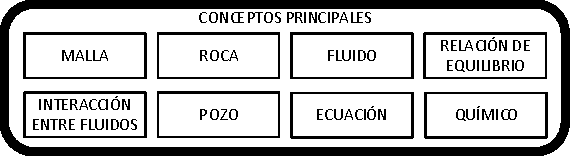
\includegraphics[width=0.9\linewidth]{Fig/Conceptos.pdf}%
	\caption[Conceptos principales en la simulación.]{Conceptos principales en la simulación. Los autores.} \label{fig:Concepts}
\end{figure}

%\subsection{Mesh}
\subsection{Malla}
Al resolver el dominio espacial continuo como un conjunto discreto de celdas (discretizar el espacio), aparecen propiedades tales como los volúmenes de las celdas y el área de las caras. Este conjunto discreto de celdas es el que se denomina como ``malla''. A su vez, la celda es un conjunto discreto de caras que generan una superficie cerrada\footnote{En el caso tridimensional}. Cada celda cuenta con una numeración, que sirve para identificar posiciones en el espacio y ubicar las vecindades correspondientes para el cálculo del flujo discretizado.\\

Una malla existe a partir de la conceptualización de los elementos emergentes en la discretización, que contiene todas las propiedades necesarias para generar el conjunto de celdas. Además, existe un actor ``geomodelador'' que se usa para definir el número de celdas en cada eje, sus espesores y topes tal como se presenta en  la Figura \ref{fig:Mesh}. Una vez se definen tales propiedades, la malla aparece en un proceso iterativo de creación de la cantidad de celdas y el respectivo cálculo de volúmenes, profundidades y numeración para cada una. Posteriormente, las caras se crean en otro proceso iterativo, conteniendo la información sobre las vecindades de cada celda, donde cada celda tiene un conjunto de caras\footnote{Es posible notar que la cara existente entre dos celdas vecinas se crea dos veces, una por cada celda.}.\\

\begin{figure}[h]
	\centering%
	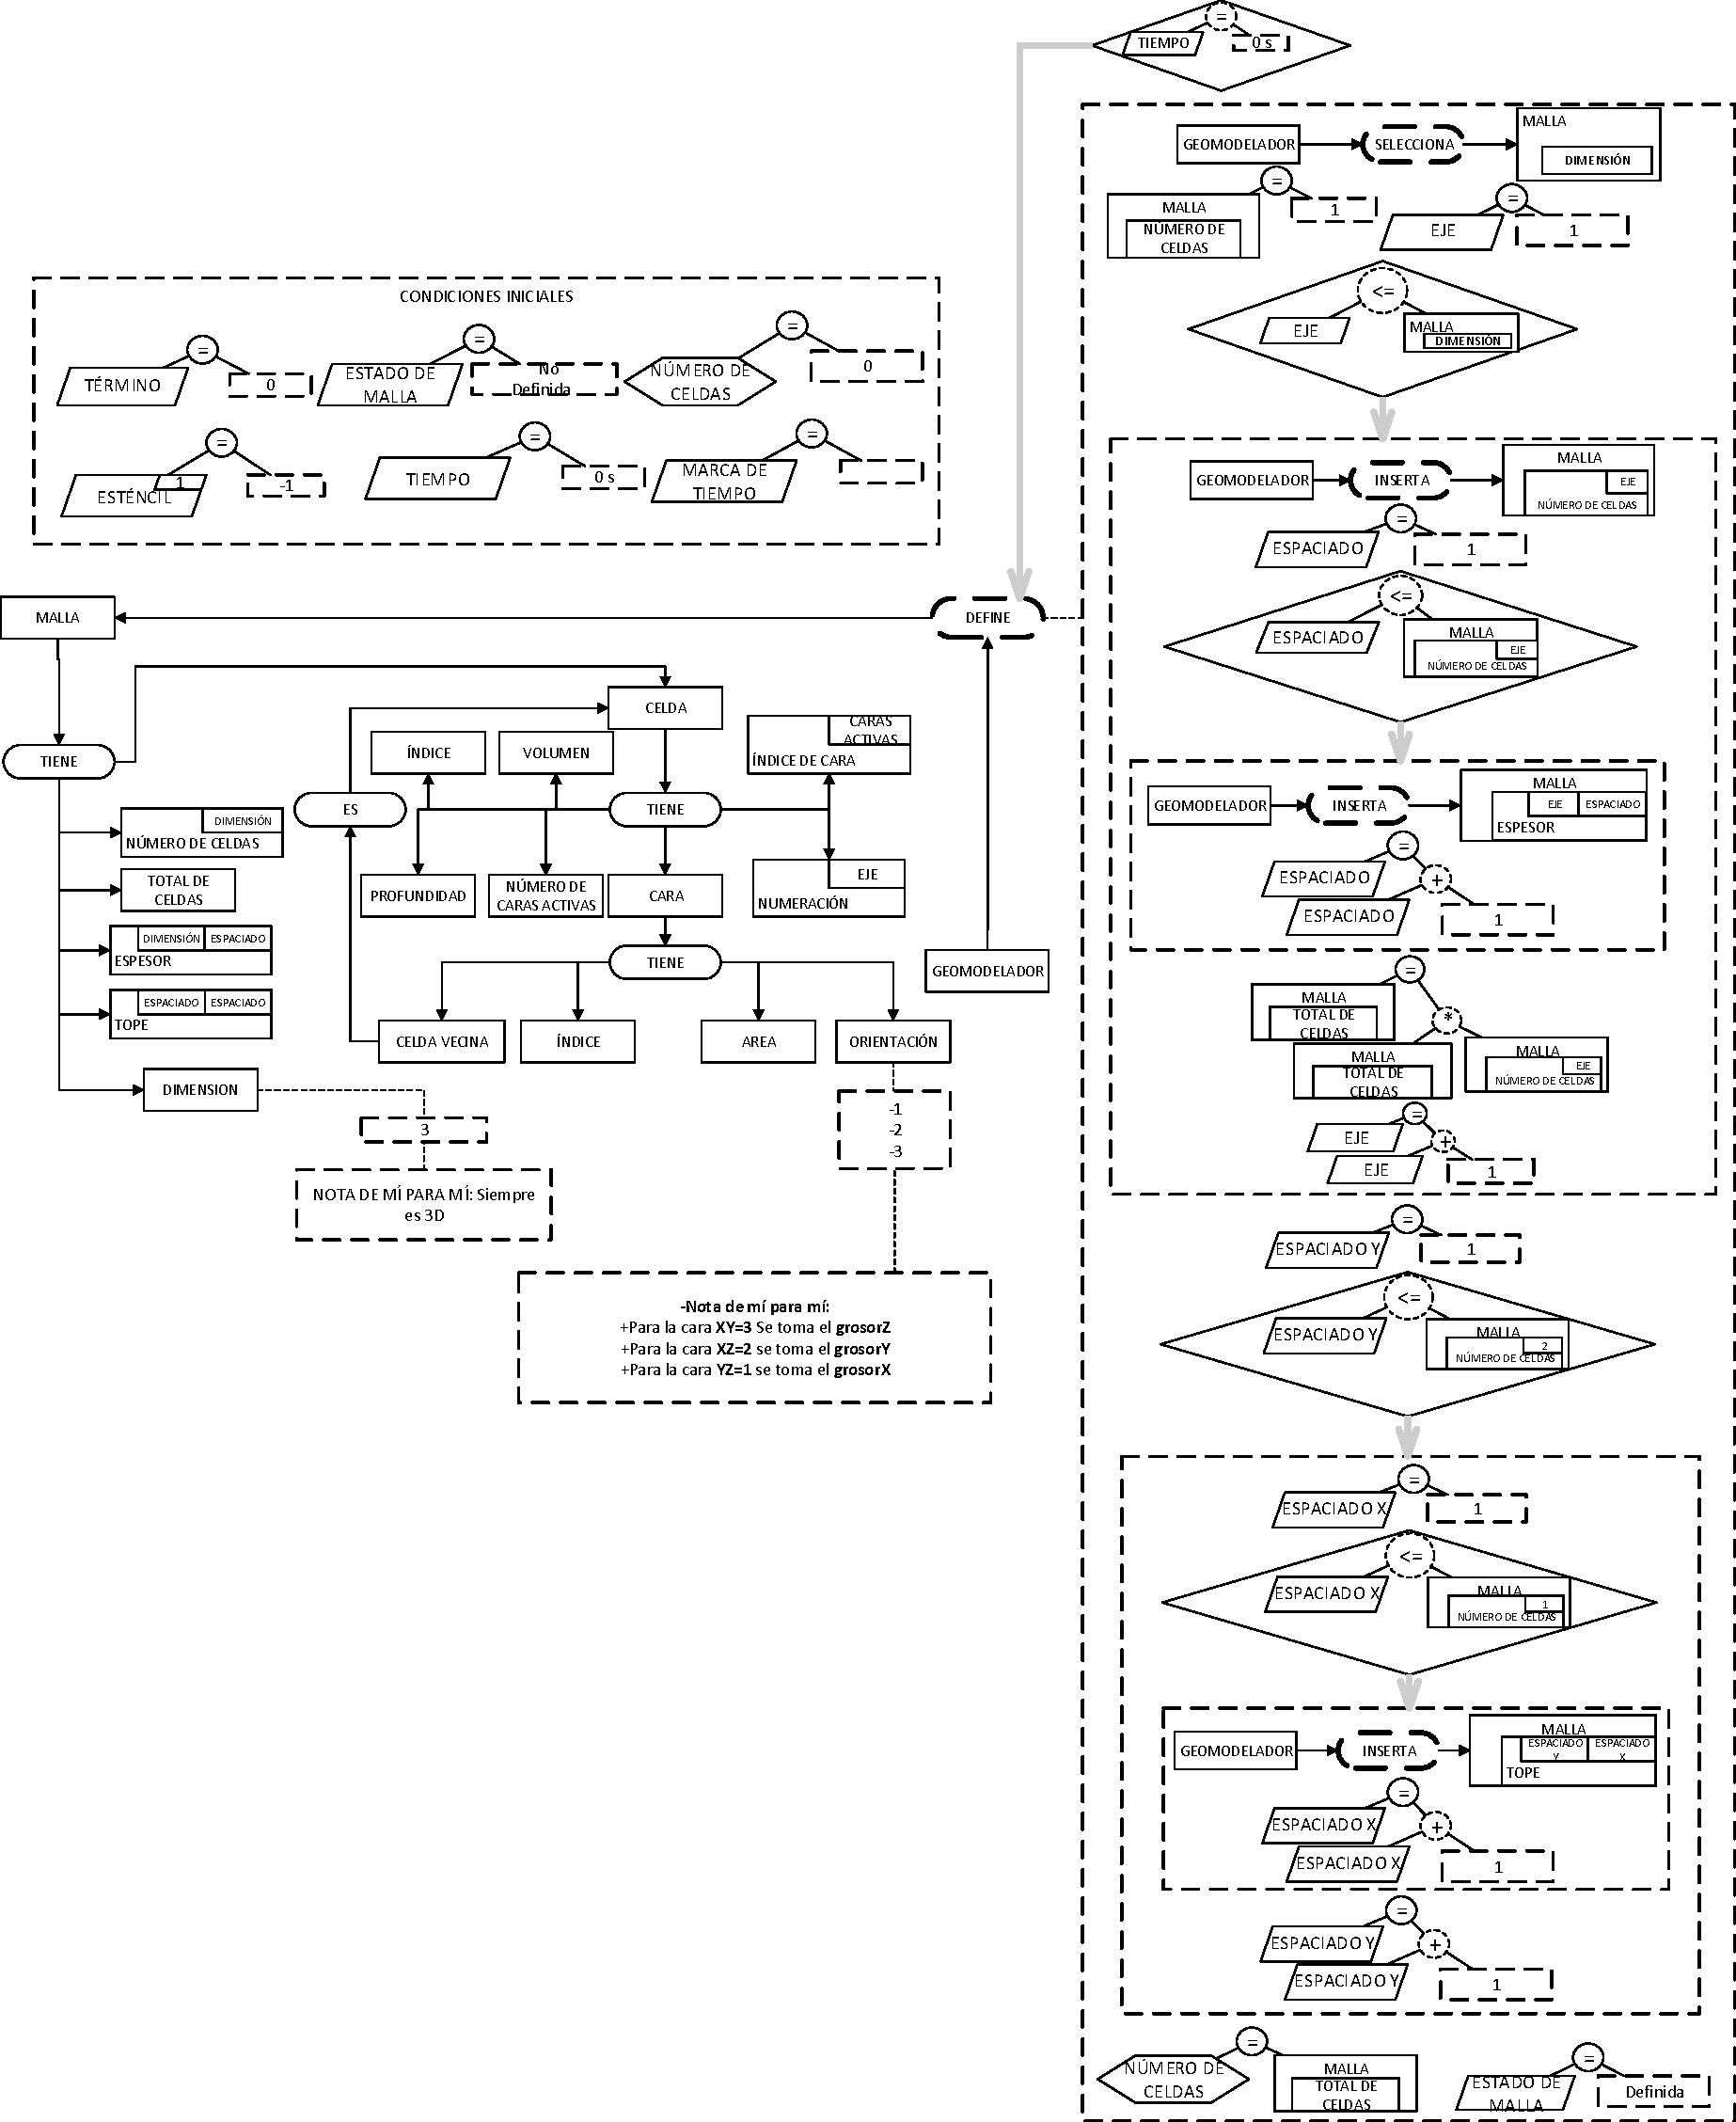
\includegraphics[width=0.9\linewidth]{Fig/Mesh.pdf}%
	\caption[Definición de la malla.]{Definición de la malla. Los autores.} \label{fig:Mesh}
\end{figure}

%Este párrafo puede servirme más para la parte del evento.


%We propose a representation of a mesh as a collection of cells which are represented likewise. collection of faces plus their respective attributes. This representation accounts for orthogonal cartesian meshes. Those are generated using the number of cells in each axis or direction, the thickness and top for each cell. Nevertheless, the thickness is only needed for the number of cells defined in every axis, because we work with regular meshes. Therefore the rest of the cells will have the same thickness.
%The top of the mesh is required for the first XY plane, and needs to be filled with the depths of each cell in that plane, the rest of the cells are calculated using the depth of the first plane.

%The representation stated for Mesh only accounts for orthogonal cartesian meshes, which can be generated with information about number of cells in each axis, their thickness and tops. A (The information above is inserted by a) Geomodeler with defines the mesh by inserting for each axis the number of cells and the thickness for cells in that direction. Once 

%\subsection{Rock}\label{sec:PS_Rock}
\subsection{Roca}\label{sec:PS_Rock}

La especificación de la relación dinámica ``Petrofísico caracteriza roca'' se especifica con la inserción de las condiciones iniciales de porosidad y permeabilidad absoluta para la roca asociada en el yacimiento. Es posible notar que estos atributos de la roca se representan como arreglos por la cantidad de términos, que se derivan de los pasos de tiempo y la cantidad de celdas definidas en la malla. Adicionalmente, el petrofísico define la compresibilidad de poro y la presión a la que ésta se mide para el cálculo de la porosidad a los términos posteriores. El modelo incluye una única roca a la cual se asignan todas las propiedades de cada una de las celdas. La caracterización de la roca se presenta en la Figura \ref{fig:Rock}.\\

\begin{figure}[h]
	\centering%
	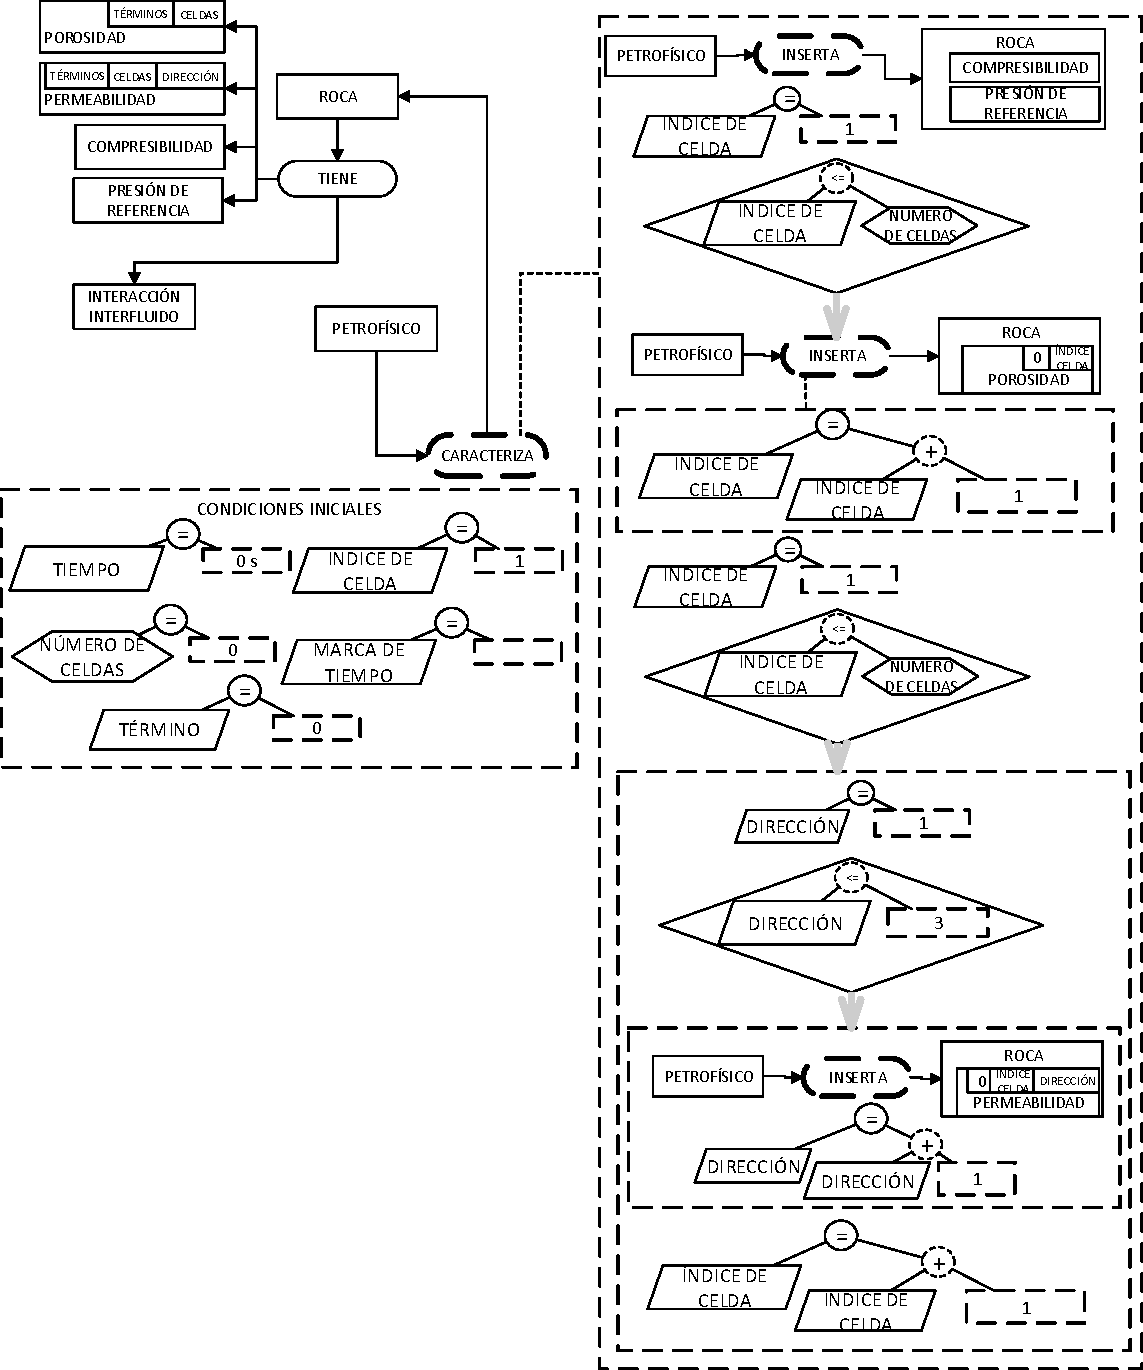
\includegraphics[width=0.90\linewidth]{Fig/Rock.pdf}%
	\caption[Caracterización de la Roca.]{Caracterización de la Roca. Los autores.} \label{fig:Rock}
\end{figure}

%\subsection{Phase}\label{sec:PS_Phase}
\subsection{Fluido}\label{sec:PS_Phase}

Los fluidos tienen propiedades que son funciones de su presión y saturación, las cuales, a su vez, son funciones del tiempo y del espacio. Así, todas las propiedades que se proponen en la conceptualización se representan como arreglos dependientes de la cantidad de términos y de la cantidad de celdas, tal como se presenta en la Figura \ref{fig:FluidProps}. La representación del fluido, su relación dinámica ``ingeniero de fluidos caracteriza fluido'' y su respectiva especificación se presentan en la Figura \ref{fig:Fluid}.\\

\begin{figure}[h]
	\centering%
	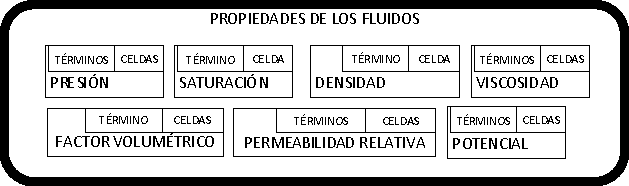
\includegraphics[width=0.9\linewidth]{Fig/PropiedadesDeFluidos.pdf}%
	\caption[Caracterización del fluido.]{Caracterización del fluido. Los autores.} \label{fig:FluidProps}
\end{figure}

\begin{figure}[h]
	\centering%
	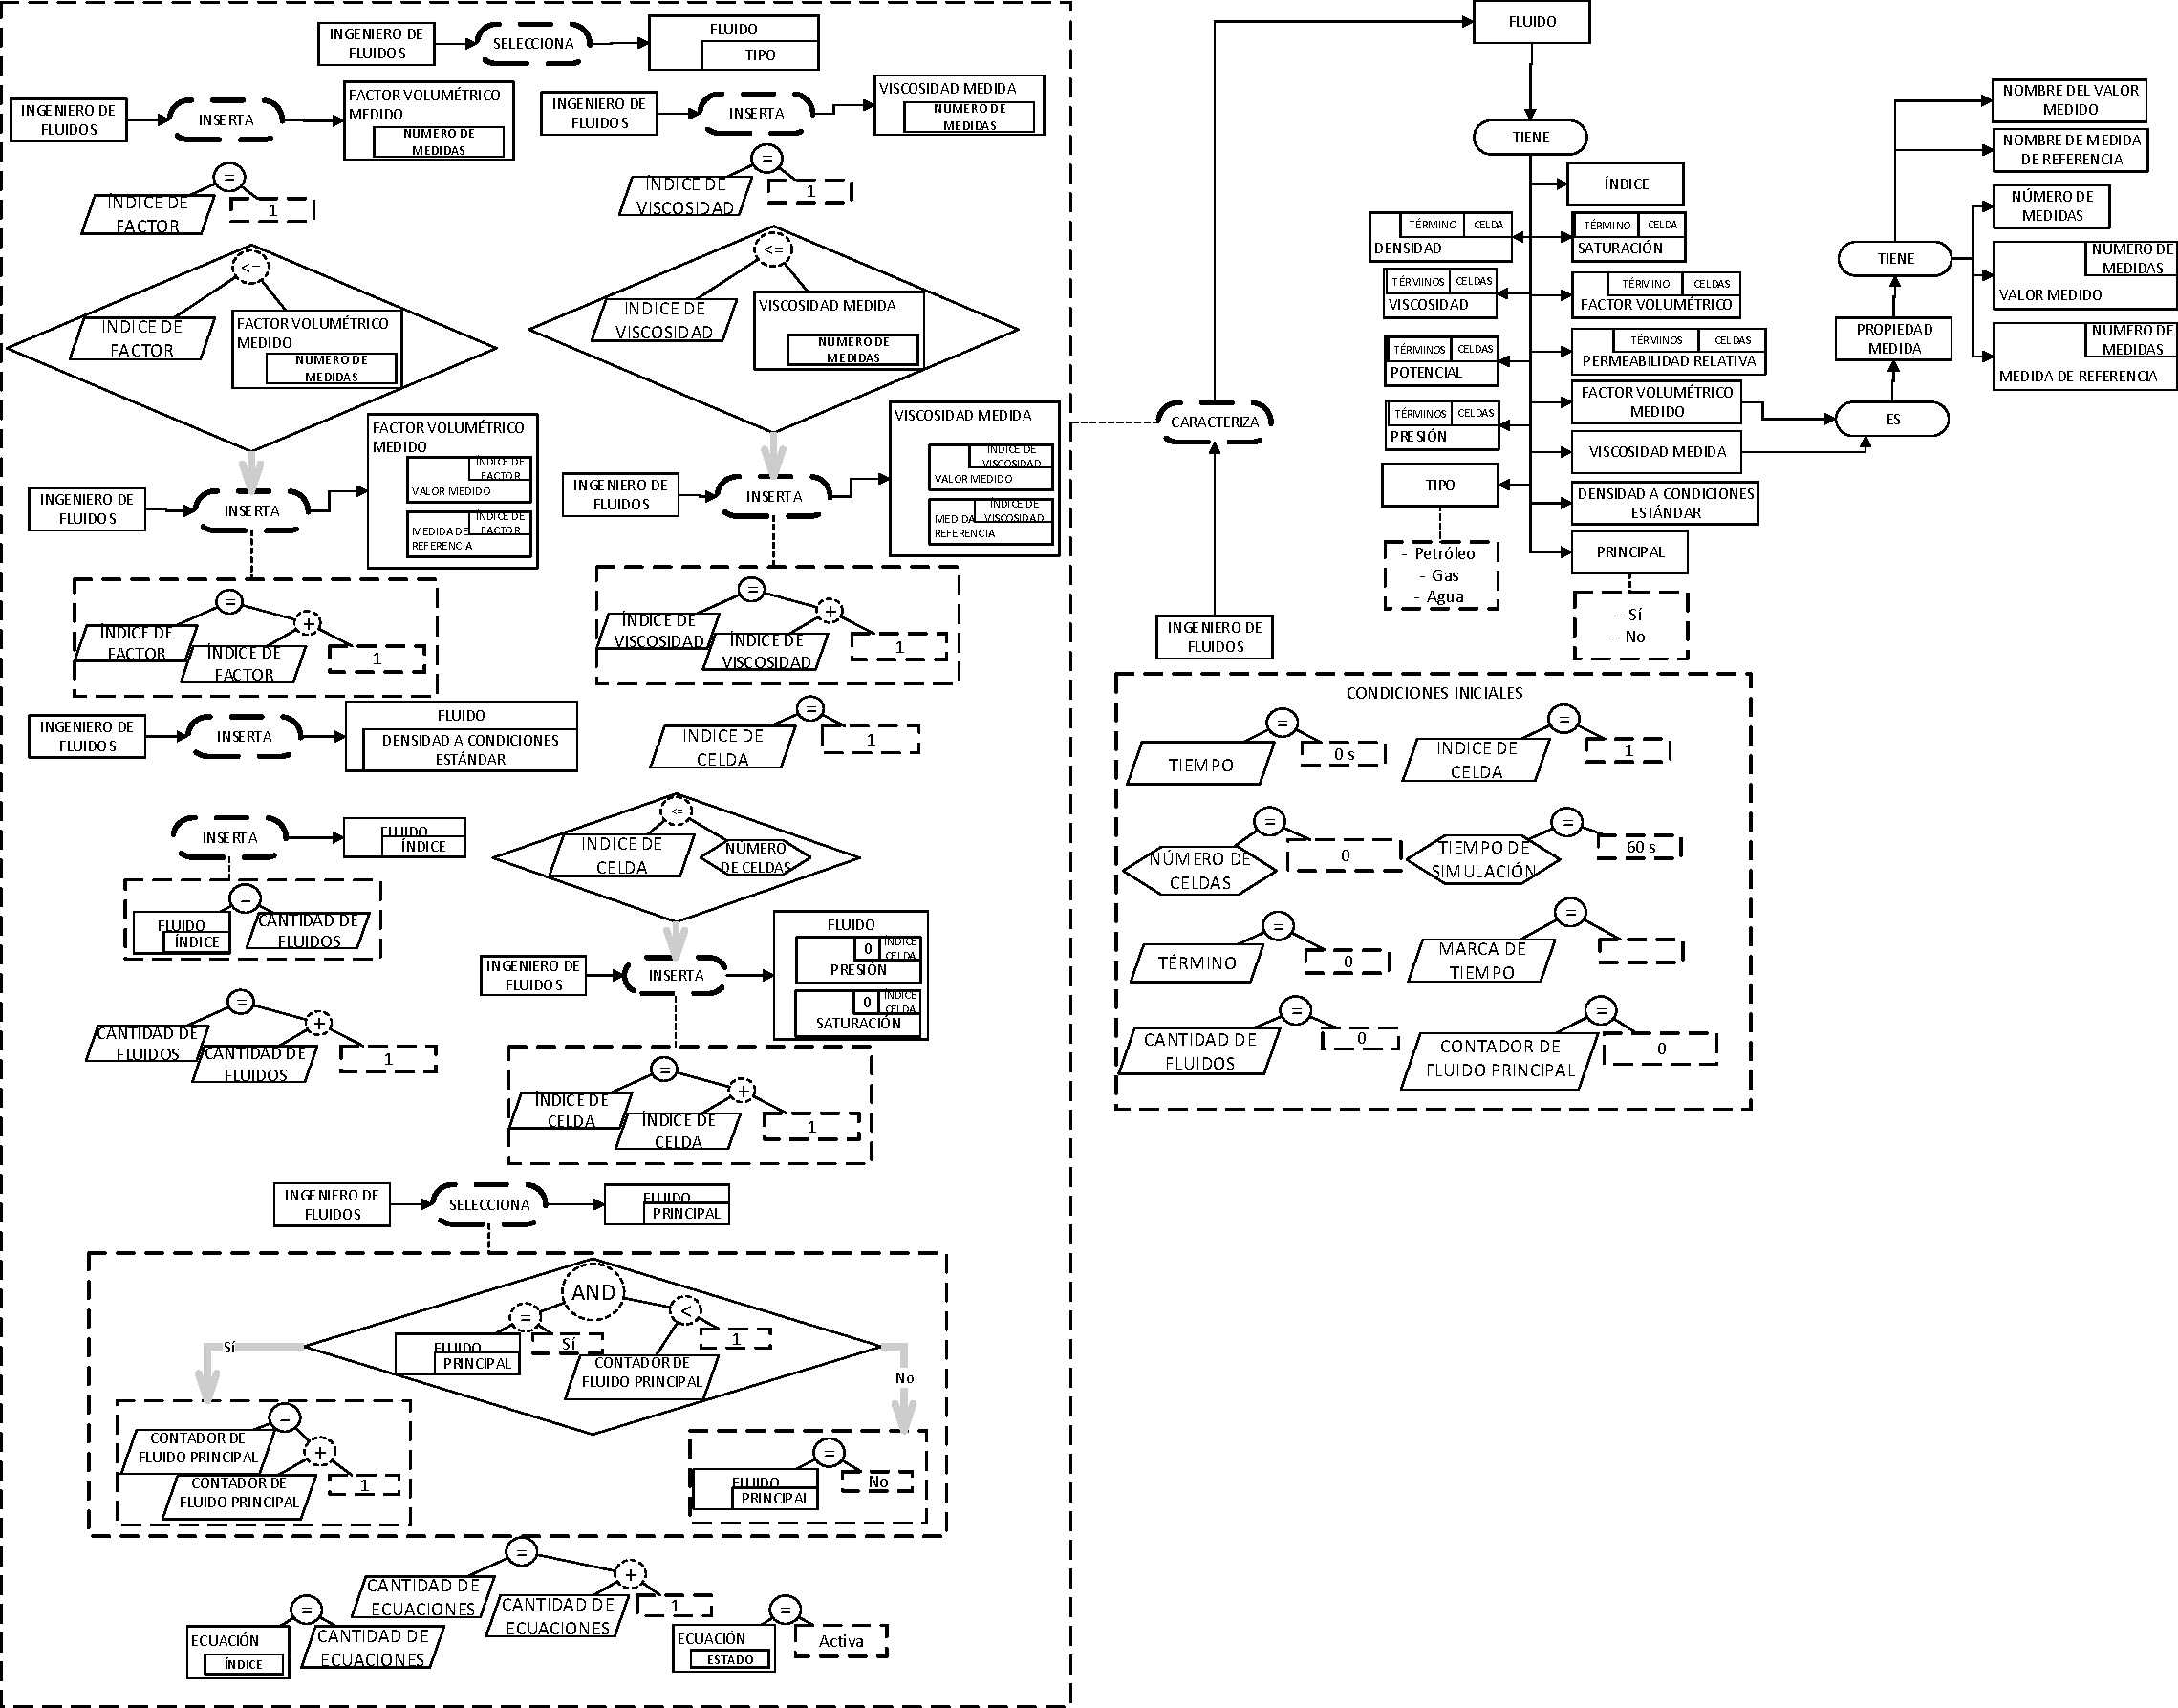
\includegraphics[width=0.9\linewidth]{Fig/Fluid.pdf}%
	\caption[Caracterización del fluido.]{Caracterización del fluido. Los autores.} \label{fig:Fluid}
\end{figure}

En pos de la generalidad, la ``viscosidad'' del fluido y su ``factor volumétrico'' se definen como funciones directas de la presión. Con este fin, aparece el concepto de ``propiedad medida'', el cuál tiene una ``medida de referencia'' y un ``valor medido'' a esa referencia. Ambos son arreglos de la ``cantidad de medidas''. En la Figura \ref{fig:Fluid} también es posible ver que el fluido tiene una ``viscosidad medida y un factor volumétrico medido''. Esto permite calcular de manera general estas propiedades, independientemente del fluido, como una interpolación en el conjunto de medidas a la presión del fluido correspondiente. El ingeniero de fluidos inserta la viscosidad medida y el factor volumétrico medido cuando caracteriza el fluido. \\

Es importante notar también, que el fluido tiene un tipo y un atributo de tipo lógico ``principal''. El tipo del fluido puede ser ``petróleo'', ``gas'' o ``agua''. Sin embargo, el fluido cuyo atributo principal sea ``sí'' o ``\textit{true}'', incluye la presión en su respectiva ecuación. Los demás fluidos incluyen su saturación. 

%\subsection{Equilibrium Relation}\label{sec:PS_Equilibrium}
\subsection{Relación de Equilibrio}\label{sec:PS_Equilibrium}
En las ecuaciones del BOM se considera existencia de masa de gas en el aceite (Rs o gas disuelto), y, en el caso del BOM extendido, la de aceite en el gas (Rv o aceite volatilizado). En el concepto ``Relación de equilibrio'', se generaliza la existencia de masa de un fluido dentro de otro fluido como un coeficiente de partición, tal como se muestra en la conceptualización (véase Sección \ref{sec:Concepts}). Se postula, también, que existe un fluido que aporta masa y otro que la recibe, tal como se ve en la Figura \ref{fig:EqRelation}. El coeficiente de partición cumple la mismas condiciones de la viscosidad o el factor volumétrico del fluido. Además, la relación de equilibrio tiene un coeficiente de partición medido. Tal definición de las relaciones de equilibrio tiene implicaciones en el cálculo de la densidad de

\begin{figure}[h]
	\centering%
	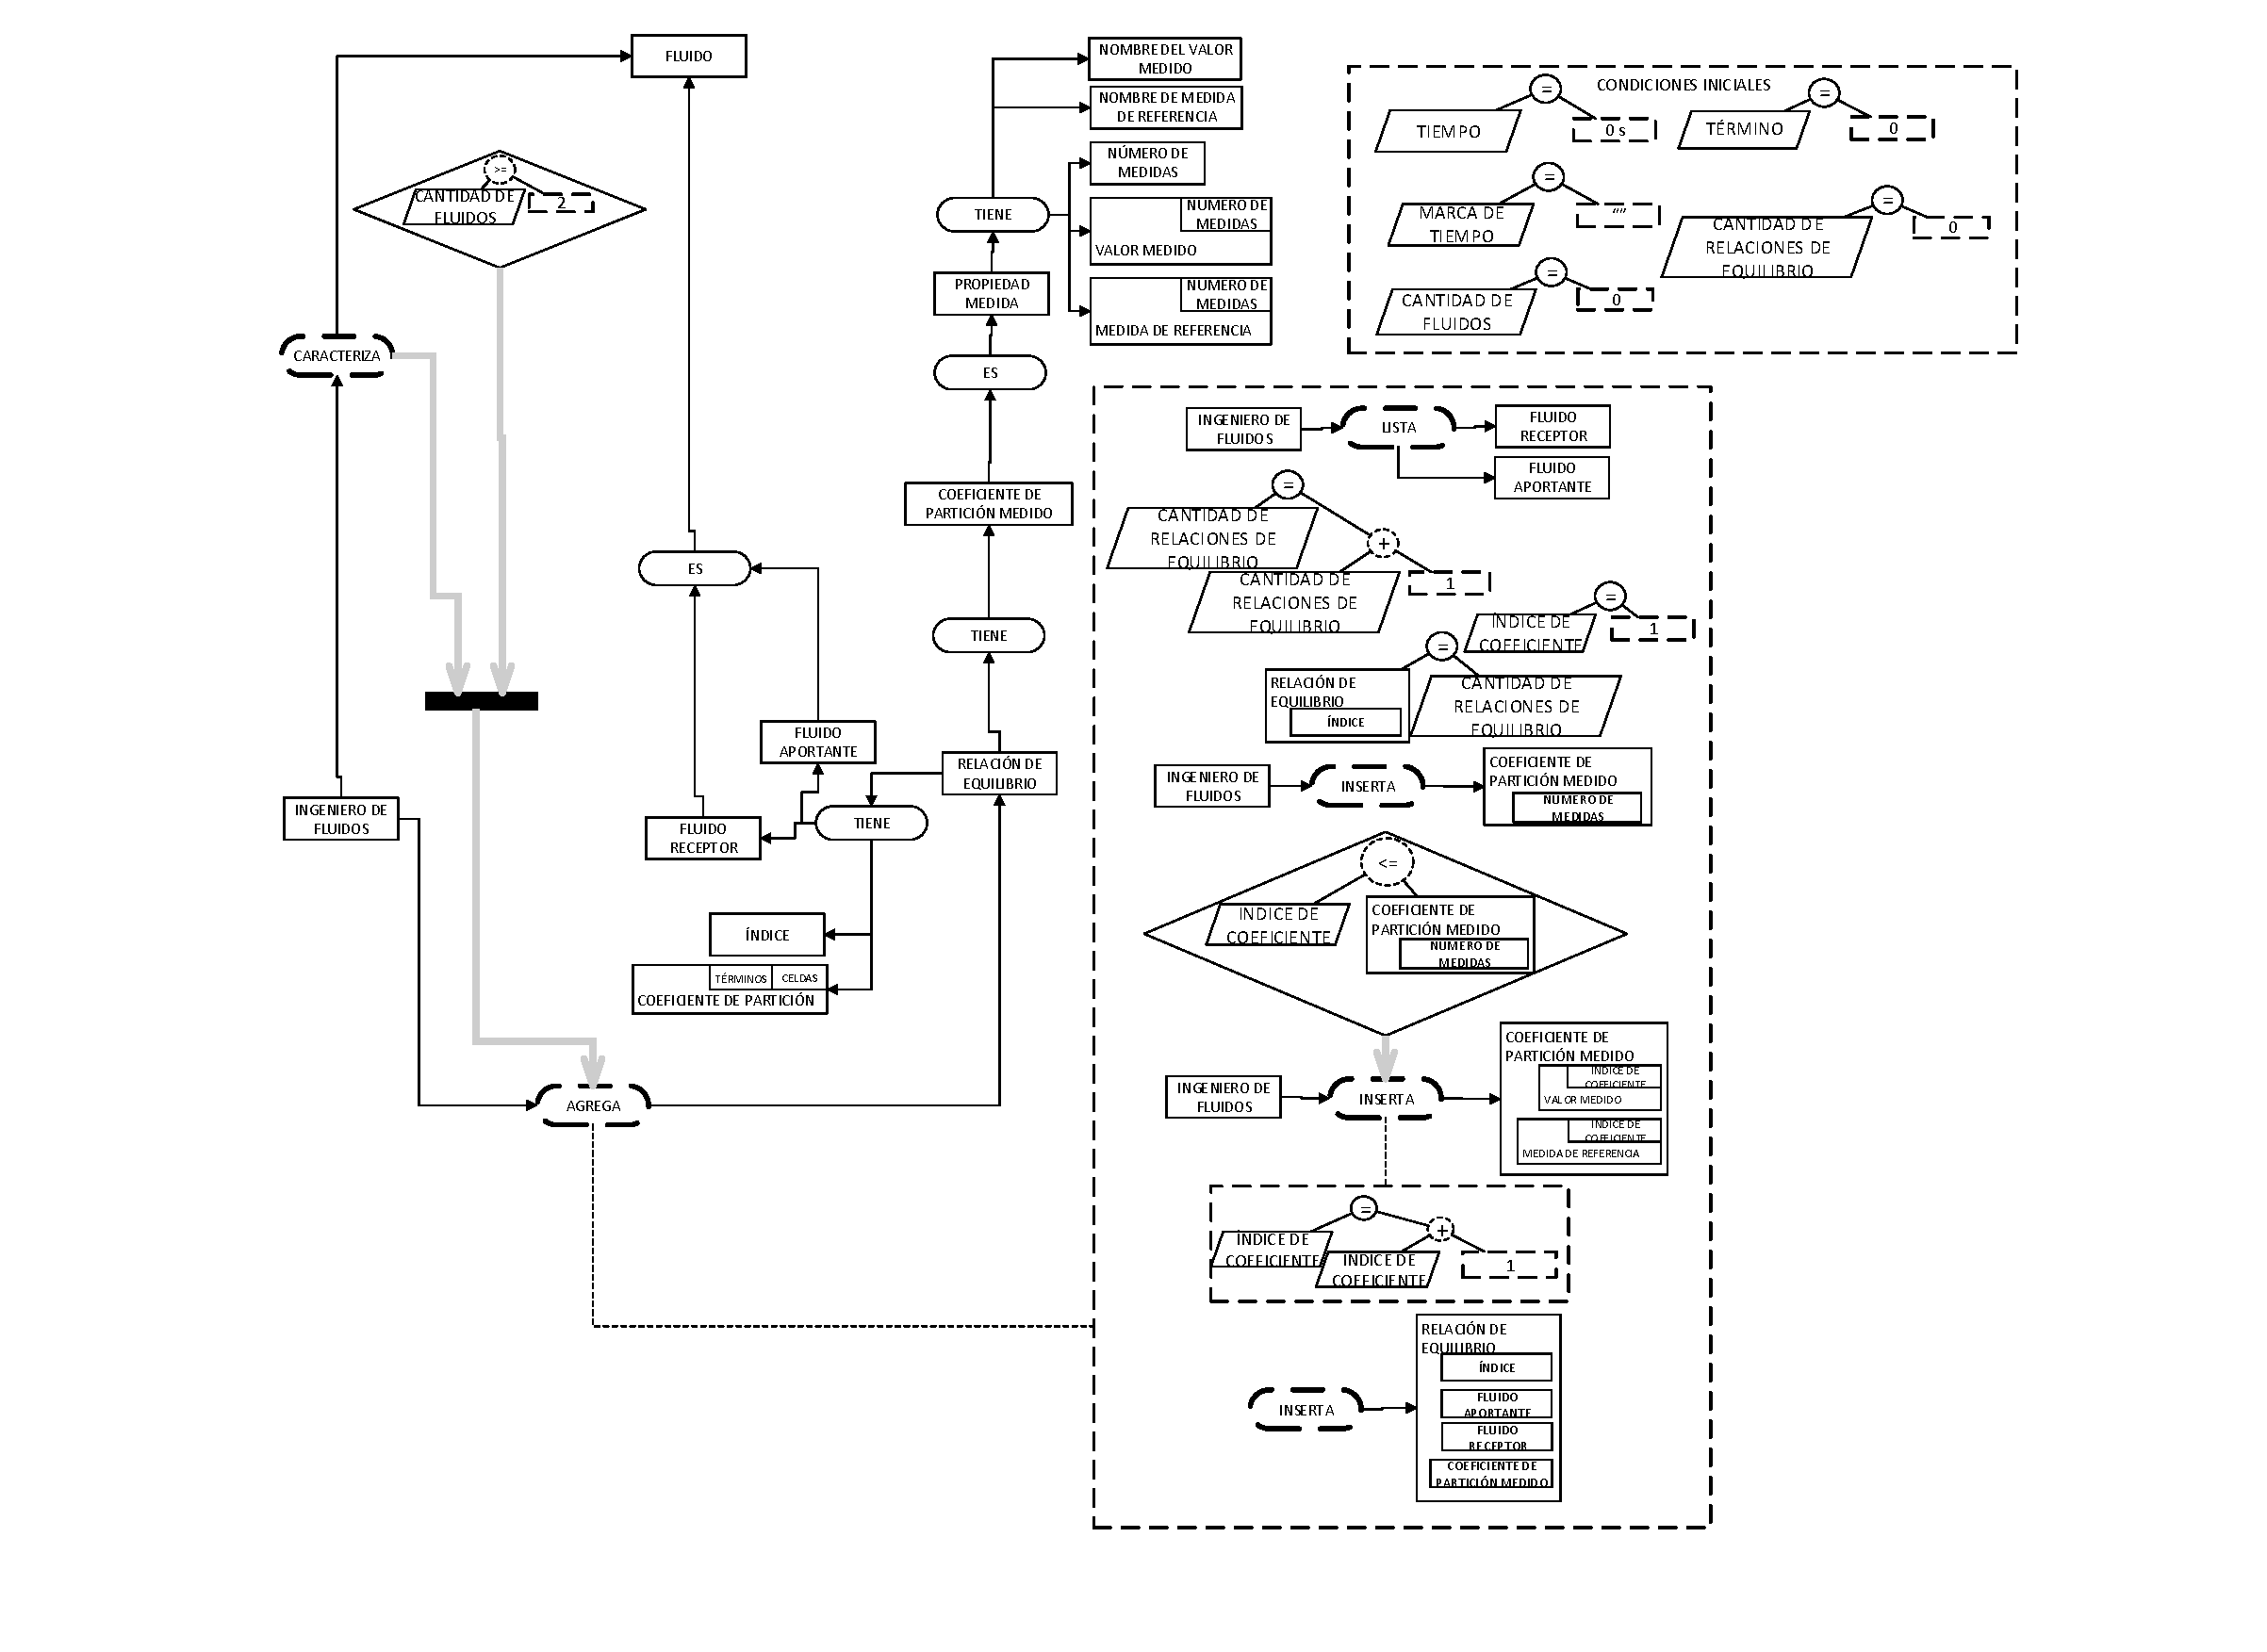
\includegraphics[width=0.9\linewidth]{Fig/Equilibrium.pdf}%
	\caption[Adición de Relaciones de equilibrio.]{Adición de Relaciones de equilibrio. Los autores.} \label{fig:EqRelation}
\end{figure}

%\subsection{Inter-phase interaction}\label{sec:PS_Interphase}
\subsection{Interacción entre fluidos}\label{sec:PS_Interphase}
%
% Qué debo mencionar acá:
% Este concepto me relaciona la presión del fluido principal con la del de referencia (Presión Capilar)
% Se espera que existan exactamente 2 para un Black Oil Model y en caso de un sistema bifásico sólo una
% Se generaliza cálculo de presiones capilares a partir de la existencia de un fluido mojante y uno no mojante.
% Se espera que uno de los dos (El fluido Mojante o el no Mojante) sea el fluido de referencia
% Todos los fluidos son claves foráneas a un fluido (No es que existan fluidos adicionales)
% Se asume que el fluido principal también es el que tiene los dos "contactos" - Hay que hablar de contactos en la conceptualización
% Las permeabilidades relativas tanto de referencia como principal y la presión capilar se interpolan a la saturación del fluido de referencia (Se verá luego).

%%%%%%%%%%%%%%%%%%%%%%%%%%%%%%%%%%%%%%%%%%%%%%%%%%%%%%%%%%%%%%%%%%%%%%%%%%%%%%%%%%%%%%%%%%%%%%%%%%%%%%%%%%%%%%%%%%%%%%%%%%%%%%%%%%%%%%%%%%%%%%%%%%%%%%%%%%%%%%%%%%%%%%%%%%%%%%%%
%NOTA: Es posible que este párrafo me sirva más para la parte de conceptualización de las Krs
%%%%%%%%%%%%%%%%%%%%%%%%%%%%%%%%%%%%%%%%%%%%%%%%%%%%%%%%%%%%%%%%%%%%%%%%%%%%%%%%%%%%%%%%%%%%%%%%%%%%%%%%%%%%%%%%%%%%%%%%%%%%%%%%%%%%%%%%%%%%%%%%%%%%%%%%%%%%%%%%%%%%%%%%%%%%%%%%
Las interacciones entre fluidos se proponen como una generalización de los contactos entre fluidos. En el caso del modelo BOM, se deben especificar dos: los contactos gas-aceite y aceite-agua. En este concepto se relacionan directamente las dependencias de la permeabilidad relativa del fluido principal con su respectivo fluido de referencia en el contacto. Además, para el fluidos cuya incógnita es la saturación, se relaciona la presión del fluido principal con su respectiva presión capilar, con el fin de calcular la presión faltante. Para esto, es necesario saber de antemano cuál fluido es el mojante y cuál es el no mojante. Adicionalmente, todas las propiedades dependientes se calculan a la saturación del fluido de referencia. En la figura \ref{fig:Contact} se presenta la representación propuesta para las interacciones entre fluidos.

\begin{figure}[h]
	\centering%
	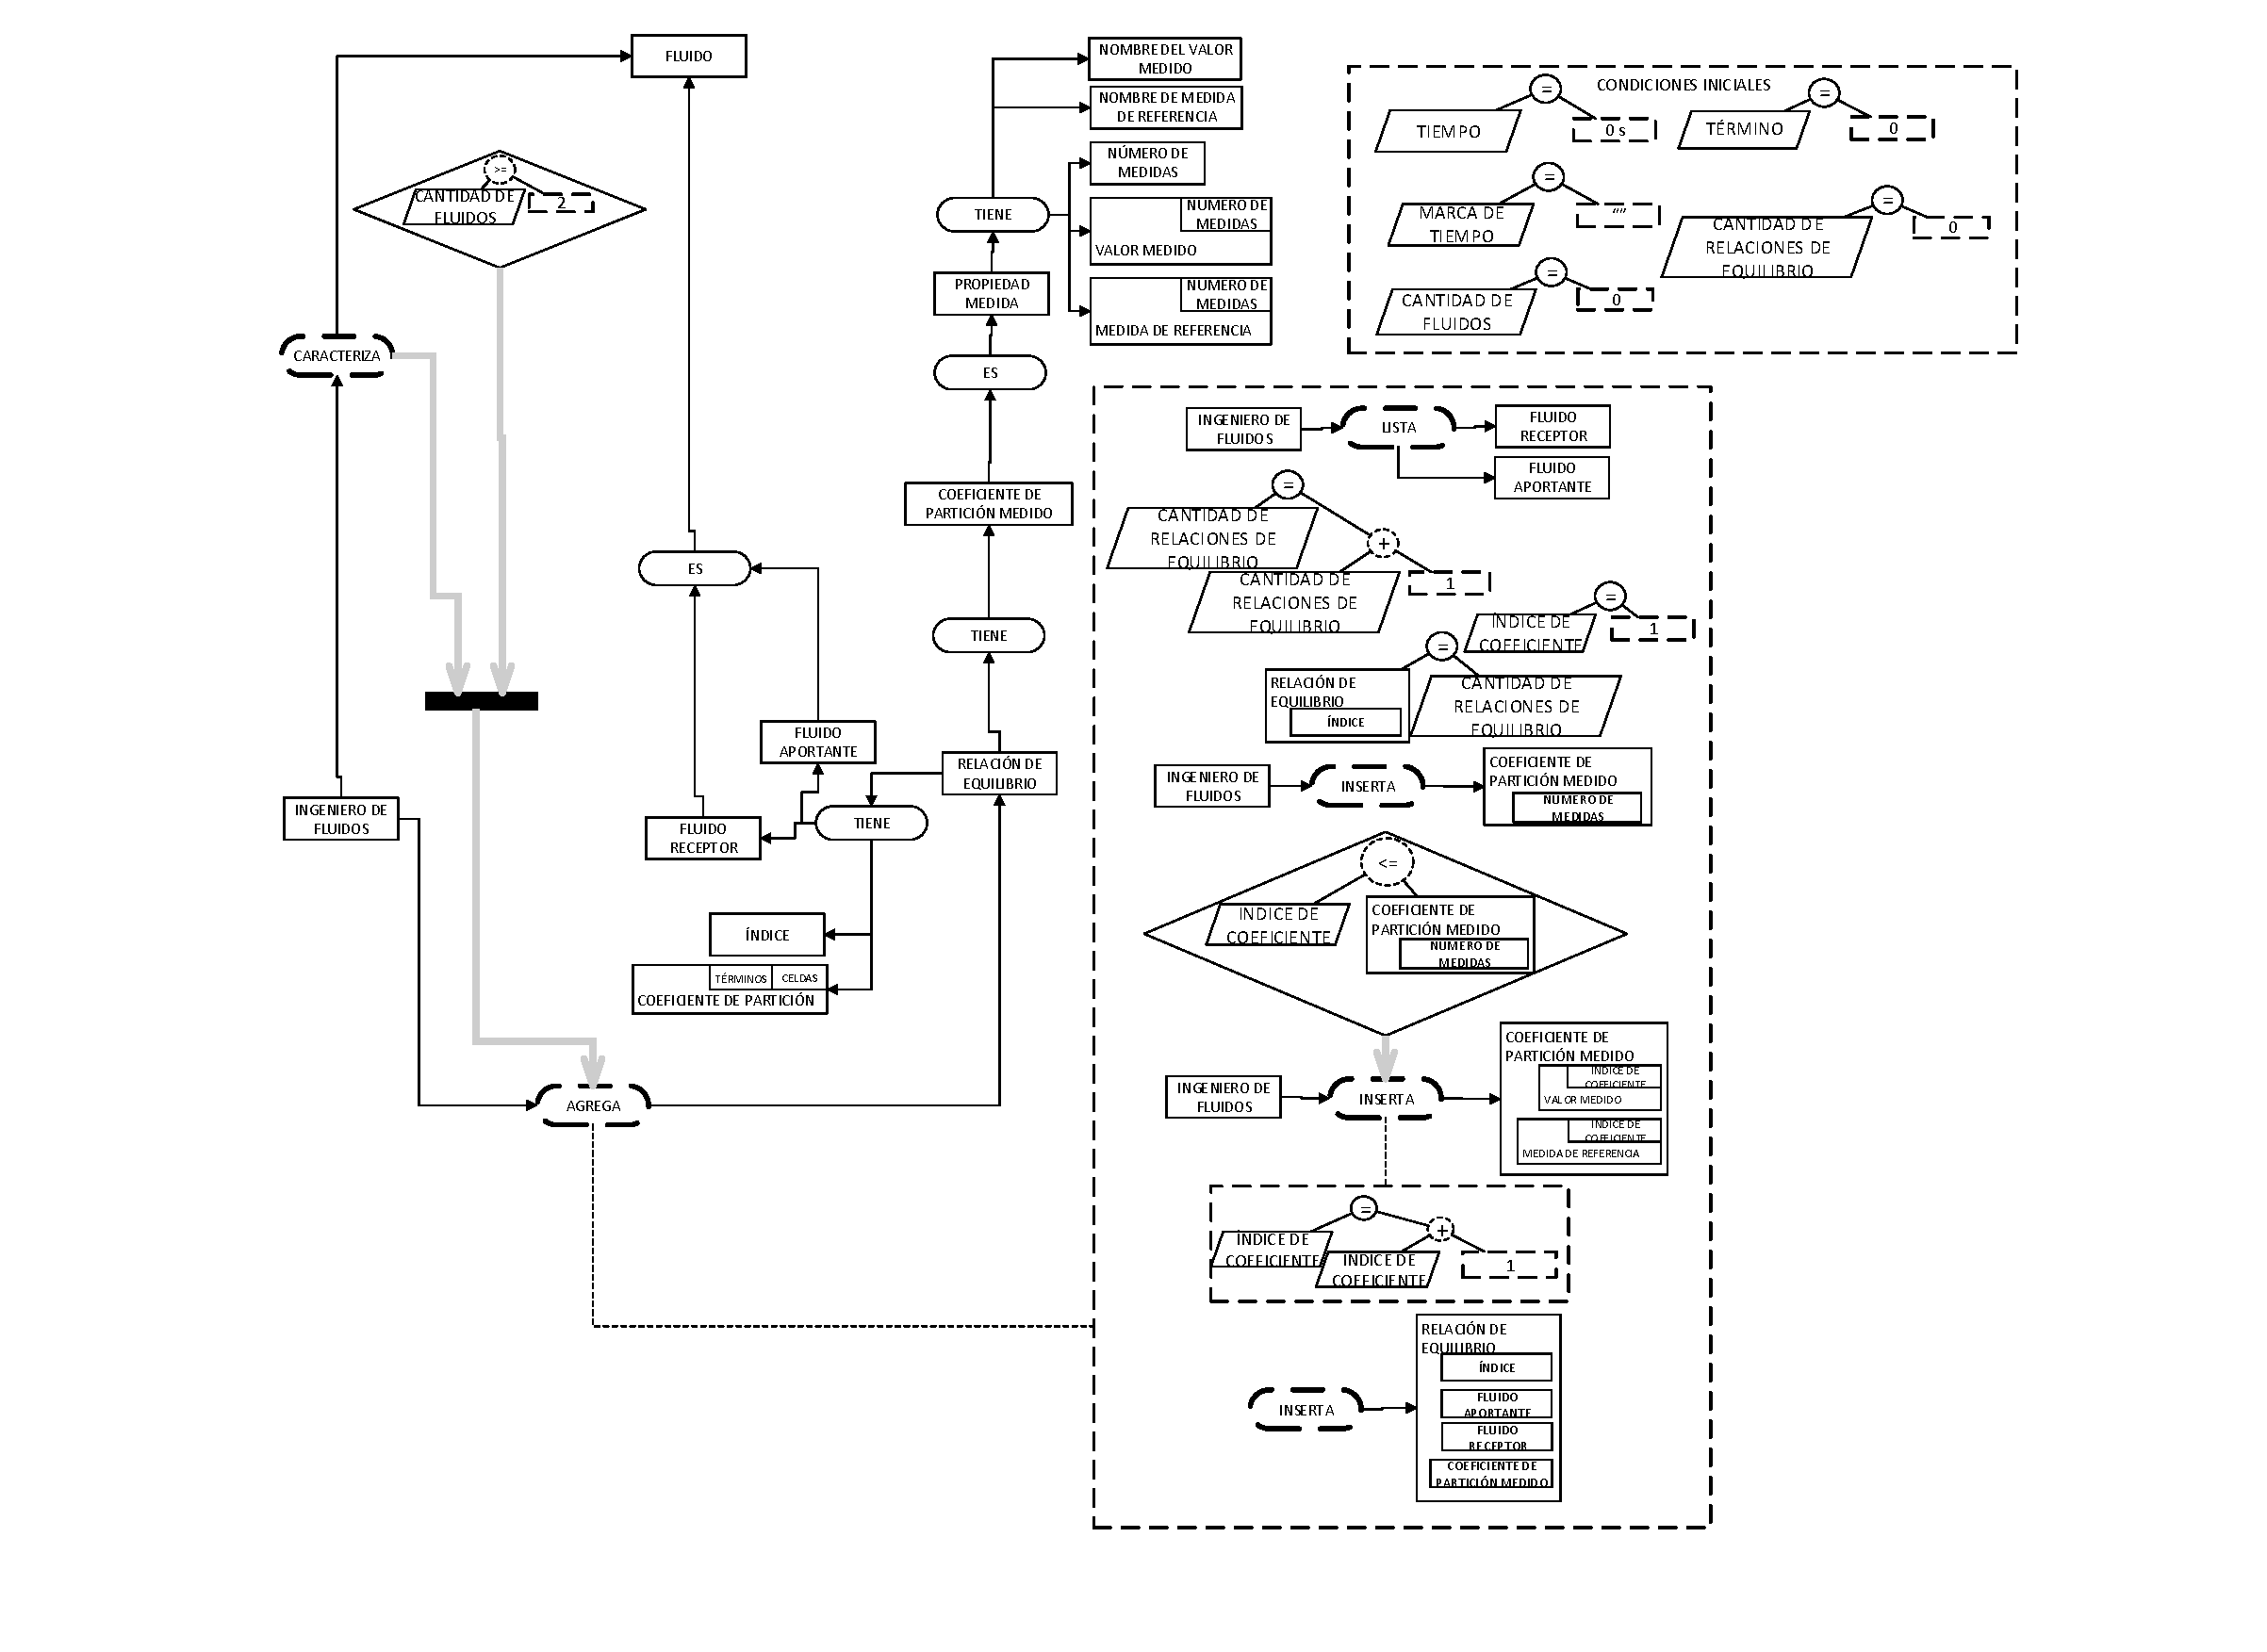
\includegraphics[width=0.9\linewidth]{Fig/Equilibrium.pdf}%
	\caption[Adición de Interacción entre fluidos.]{Adición de Interacción entre fluidos. Los autores.} \label{fig:Contact}
\end{figure}
%este concepto me relaciona un fluido de referencia, que se espera diferente del fluido con la propiedad de ser ``Principal'' y es respecto al cual se interpolarán las permeabilidades relativas, tanto propias como del fluido principal.
%\subsection{Component}\label{sec:PS_Component} % This could be changed to Chemical
%\subsection{Well}\label{sec:PS_Well}
\subsection{Pozo}\label{sec:PS_Well}
Se proponen los pozos, de manera análoga a la malla, como un conjunto de perforados que a su vez tienen atributos adicionales como lo son la presión de fondo y el caudal. Estos pozos, tienen una caracterización distinta según el tipo, sea productor o inyector. Además, es posible notar que el pozo es un concepto abstracto, de cuál se instancia uno de los dos tipos. Más aún, los perforados dependerán del tipo de pozo, siendo estos también abstractos, con sus respectivos tipos ``perforado inyector'' o ``perforado productor''. En la figura \ref{fig:Well} se presenta la representación de los pozos.\\

\begin{figure}[h]
	\centering%
	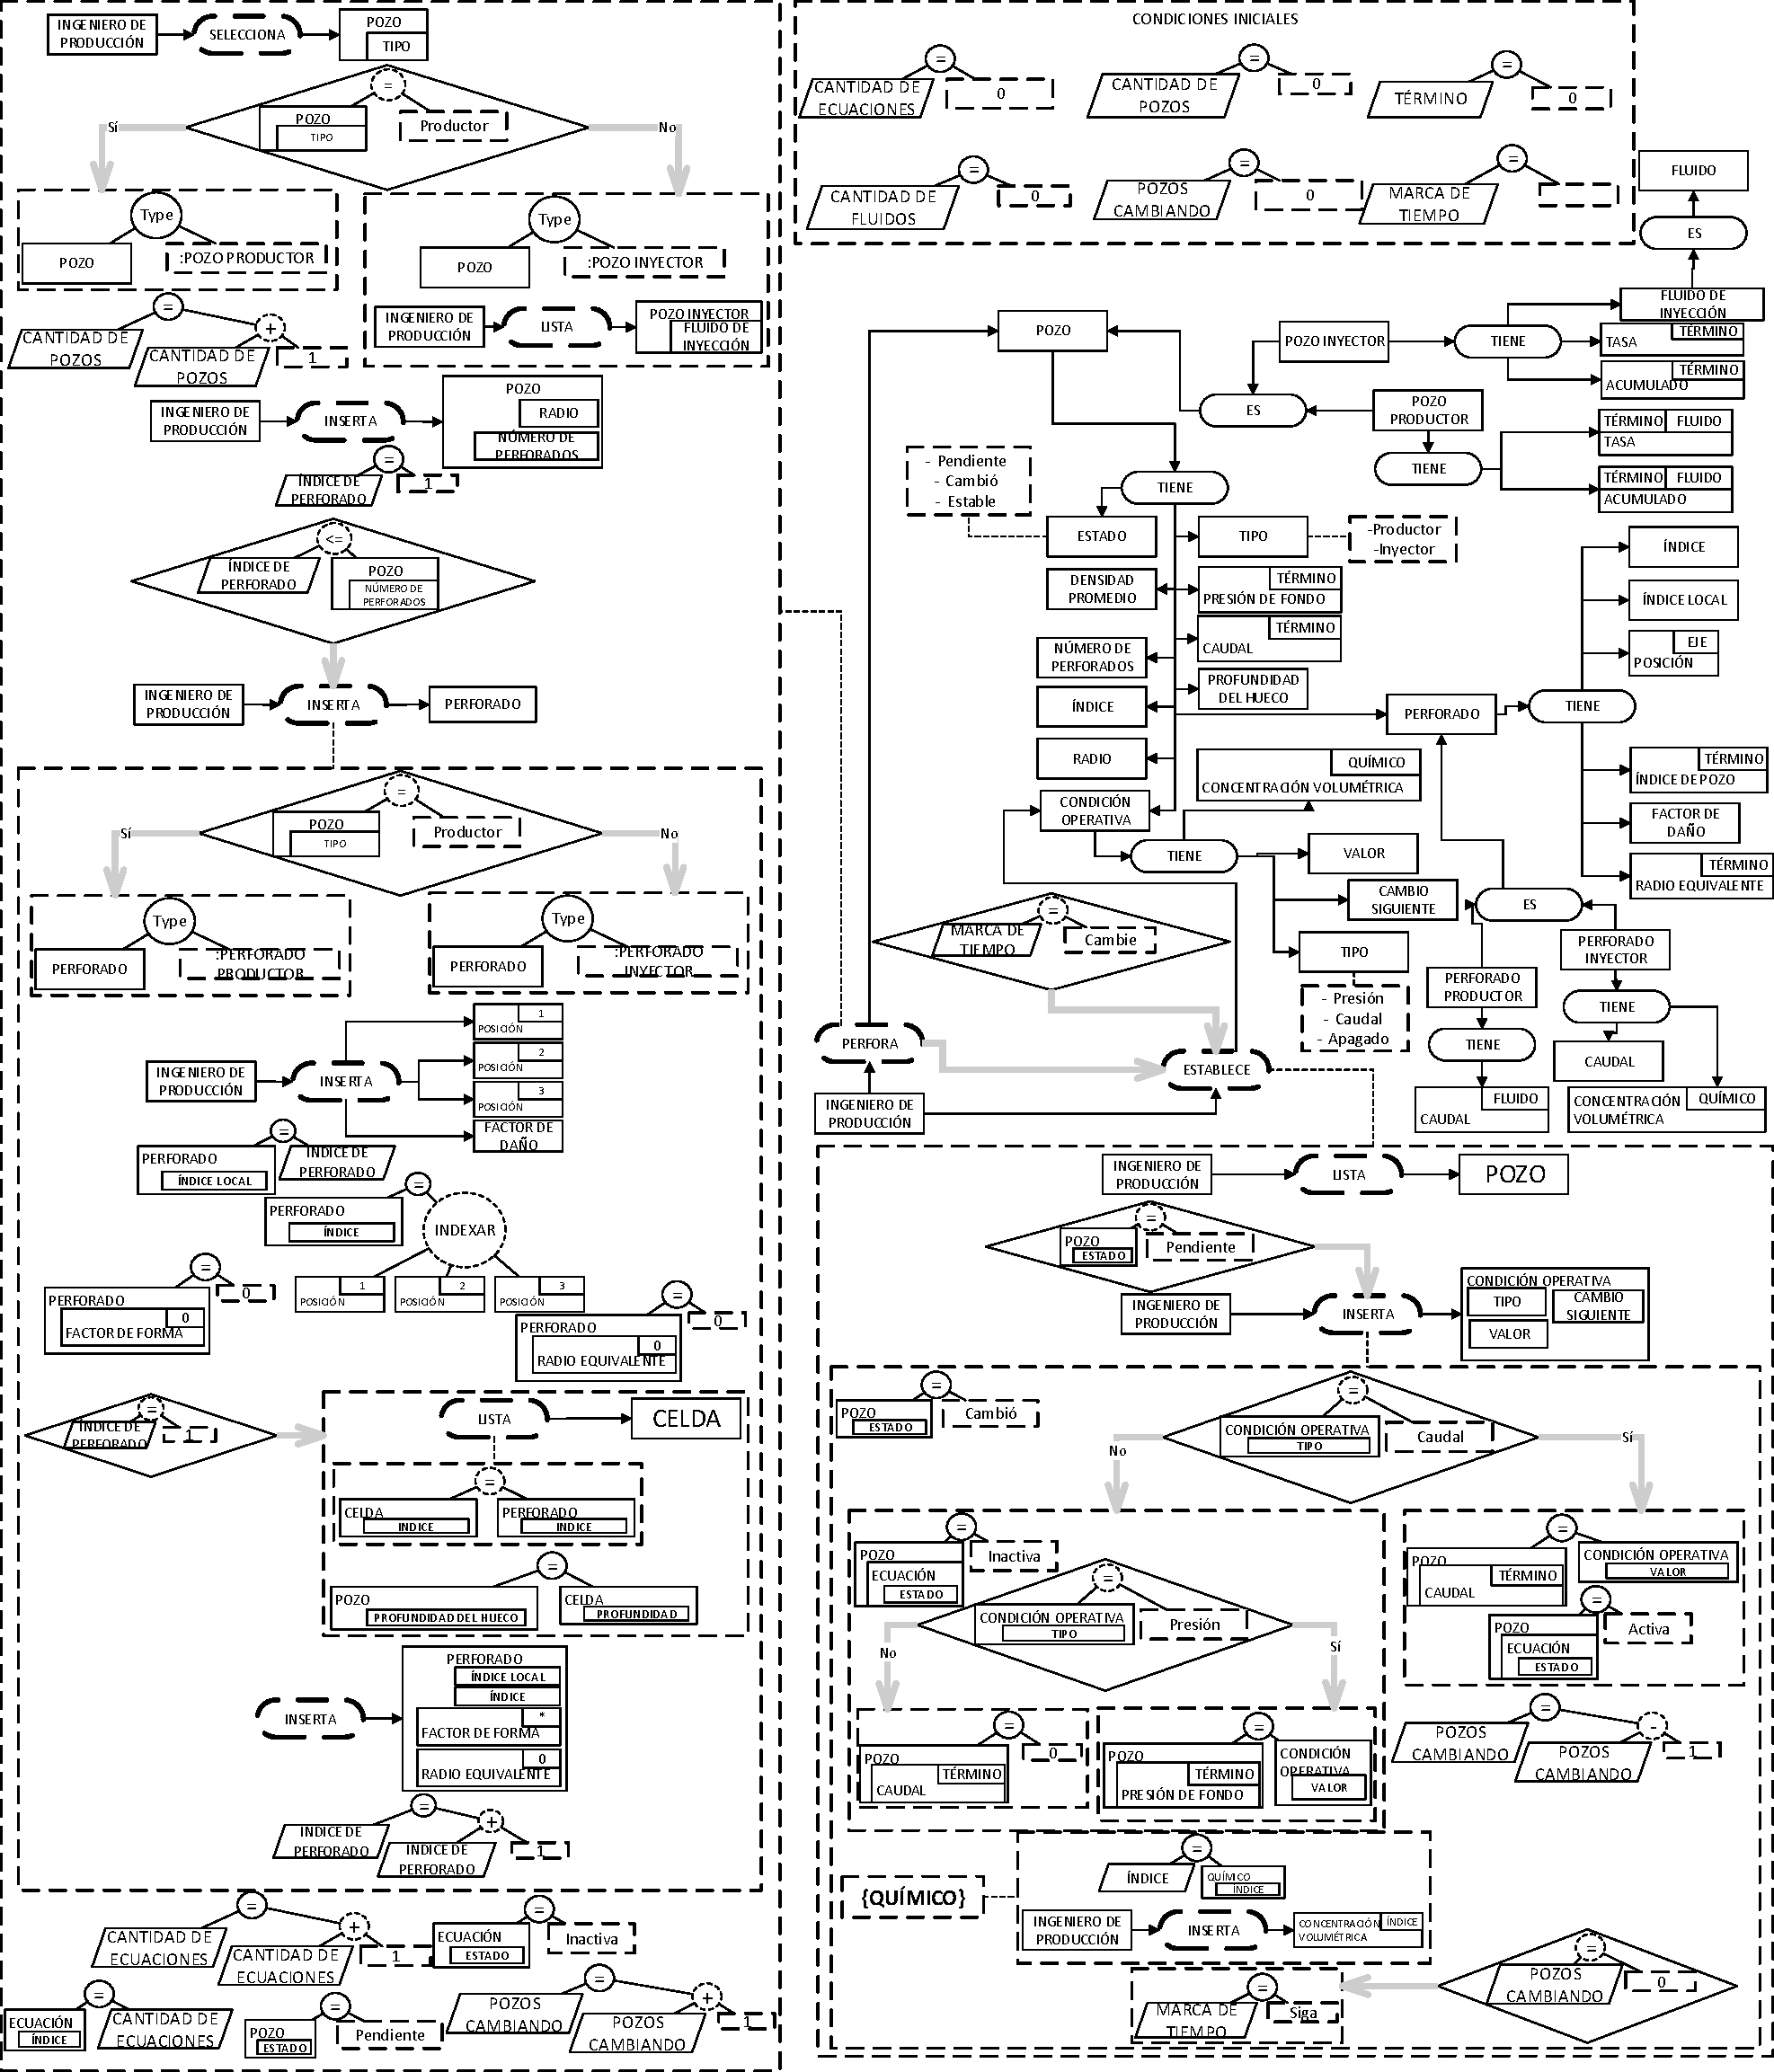
\includegraphics[width=0.9\linewidth]{Fig/Pozo.pdf}%
	\caption[Perforación de Pozos.]{Perforación de Pozos. Los autores.} \label{fig:Well}
\end{figure}

La principal diferencia entre los pozos productores e inyectores radica en que el pozo inyector tiene un fluido de inyección. Además, la tasa y el acumulado del pozo inyector sólo dependen de este fluido, mientras que para el pozo productor dependerá de la cantidad de fluidos caracterizados. Estos pozos están sujetos a la restricción de no cambiar su tipo, además para un pozo productor, su conjunto de perforados corresponderá también a perforados productores. Así mismo para los pozos inyectores.\\

Los pozos funcionan bajo una condición operativa, que permite regular la presión o el caudal al que estos inyectan o producen fluido. Estas condiciones definen si un pozo genera una ecuación (Peaceman), o si su caudal se puede resolver directamente usando la presión de fondo. Por otro lado, las condiciones operativas pueden variar en el tiempo, por lo que se requiere calcular o resolver el atributo que no está sujeto a la condición operativa cada que se establezca un cambio en esta. Adicionalmente, se reconfigura la simulación cada que se establezca un cambio en la condición operativa.

\subsection{Ecuación}\label{sec:PS_Equation}
La ecuación es un concepto agrupador, tanto el fluido como el pozo son ecuaciones (Posteriormente los químicos). Sirve para iterar sobre todos los conceptos que generan un residual en el método de Newton. Tienen un índice y estado. Este último permite que todos los pozos generen ecuación pero no necesariamente se resuelva en el jacobiano. Sólo se resuelven las ecuaciones cuyo estado sea ``activo''. (Se verá más adelante).
%Poner ecuación acá con Volumen de celda ya como concepto

%\subsection{Rock}

%\section{PS Representation of Enhanced Oil Recovery Simulation}\label{sec:PS_EOR}
\section{Representación en EP de la simulación de procesos EOR}\label{sec:PS_EOR}
En esta sección se propone una representación basada en un EP para procesos EOR. En el esquema \ref{fig:PSComplete} se evidencia la solución del BOM discretizado usando volúmenes finitos en una malla cartesiana ortogonal. El paso a paso en la ejecución de los eventos se muestra en \ref{fig:EventsInteraction}.  En el evento ``Presión del fluido varía'' se desarrollan las iteraciones del método de Newton-Raphson e internamente las iteraciones sobre las celdas requeridas para solucionar el sistema algebraico resultante de la discretización. En las secciones siguientes se explica el EP elaborado en las respectivas porciones correspondientes a eventos, subrutinas y funciones que procesan la simulación de procesos EOR. \\

Para el correcto desarrollo de la simulación, se establecen las siguientes precondiciones: existe una única malla y una única roca. En el caso de una simulación de dos fluidos debe existir una única interacción entre fluidos. En el caso de tres fluidos deben existir exactamente dos interacciones entre fluidos.


%In this section we propose a PS representation for enhanced oil recovery simulation, we couple a black oil model discretized using finite volumes method with the theoretical framework developed the previous chapter. We mapped each term in the resultant equations to their respective concepts and how they are linked together. The complete representation is shown in \ref{fig:PSComplete}.\\
\begin{figure}[h]
\centering%
\includegraphics[width=0.9\linewidth]{Fig/PozosConEcuacion.pdf}%
%\caption{Complete PS Representation for EOR Processes} \label{fig:PSComplete}
\caption[Representación en EP de la simulación de procesos EOR.]{Representación en EP de la simulación de procesos EOR. Los autores.} \label{fig:PSComplete}
\end{figure}

\begin{figure}[h]
	\centering%
	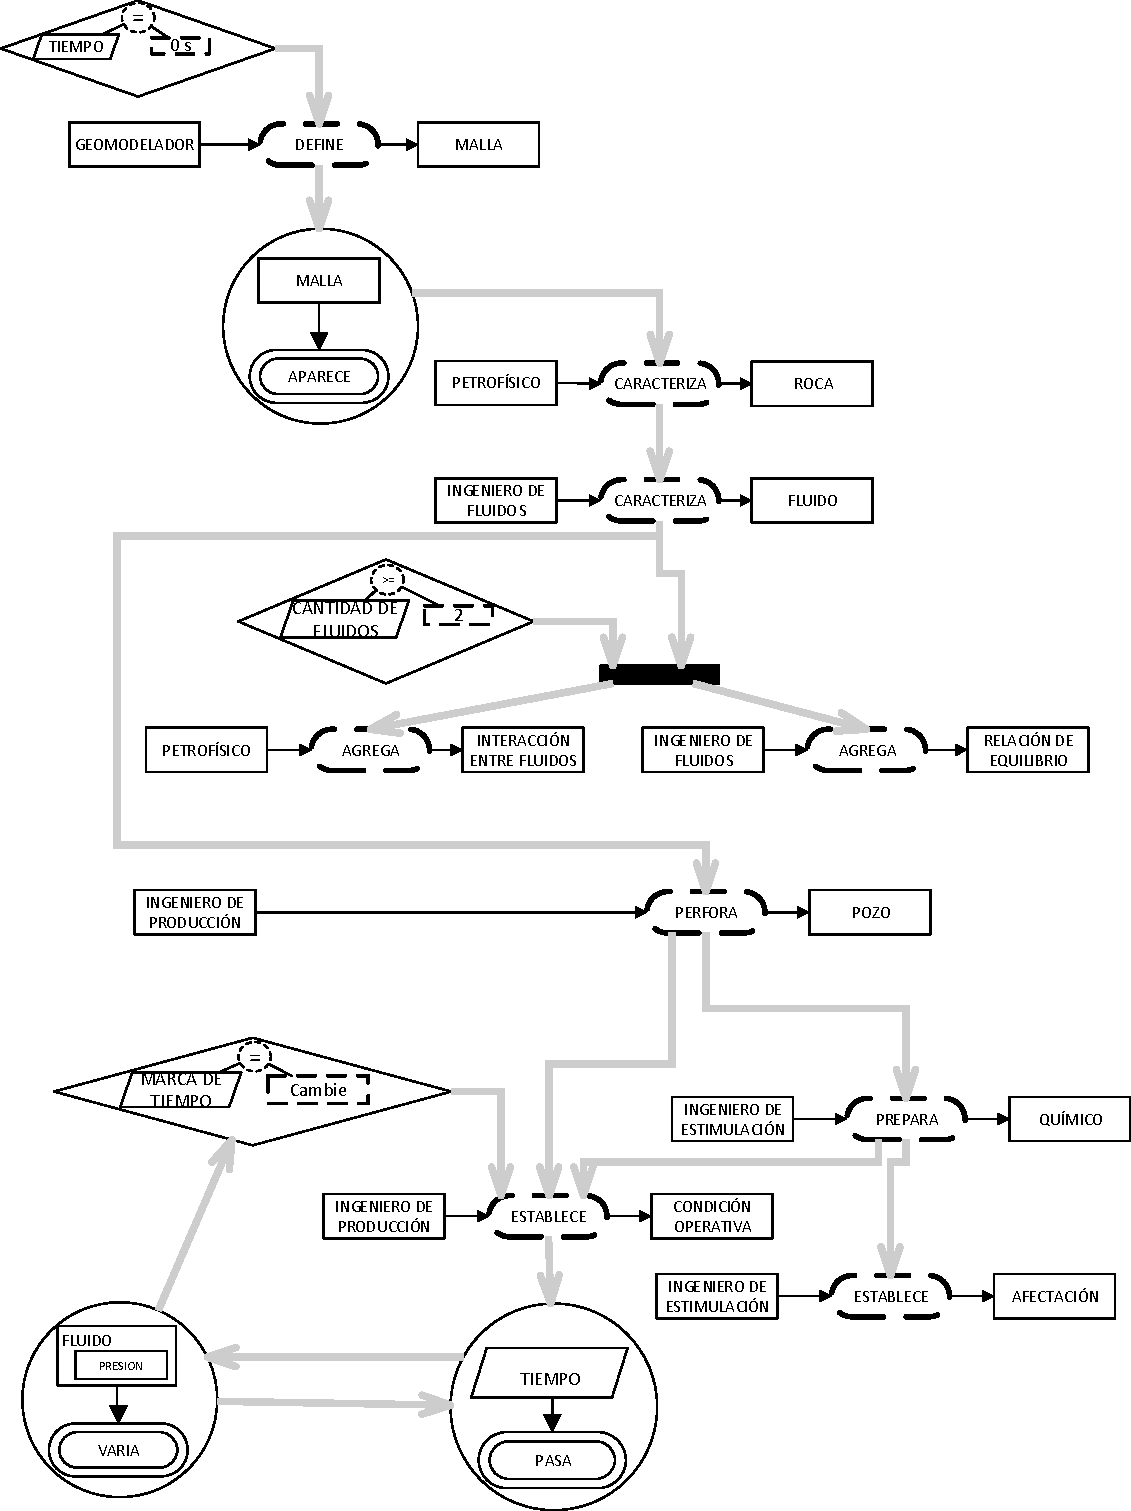
\includegraphics[width=0.9\linewidth]{Fig/FlujoDeEventos.pdf}%
	%\caption{Complete PS Representation for EOR Processes} \label{fig:PSComplete}
	\caption[Diagrama basado en el grafo de interacción de eventos.]{Diagrama basado en el grafo de interacción de eventos. Los autores basados en \cite{zapata2013Eventos}.} \label{fig:EventsInteraction}
\end{figure}
%The rest of this section is as follows: In section \ref{sec:PS_Mesh} we present the Mesh concept as a collection of cells with additional elements needed for calculating the attributes of each cell. Furthermore, we develop the dynamical relationship ``Geomodeler defines Mesh'' as an interaction of the role ``Geomodeler'' with atomic\footnote{atomic as is stated by \cite{AG01} (Aca debe ir Zapata)} dynamical relationships. In section \ref{sec:PS_Rock} we present the Rock concept with its attributes and initial characterization. In section \ref{sec:PS_Phase} ... In section \ref{sec:PS_Interphase} ... In section \ref{sec:PS_Equilibrium} we define the partition coefficients as relations between two phases, one contributing mass and another receiving mass in the mass balance equation. In section \ref{sec:PS_Well}
\subsection{Malla aparece}\label{sec:PS_MeshAppears}
El evento ``Malla aparece'' Se dispara cuando el estado de la malla es ``Definida'', que sucede justo después de que el geomodelador defina la malla. En este evento, se desarrollan dos ciclos principales. El primer ciclo es anidado por cada eje coordenado, y en total se recorre el número de celdas a definir. En este ciclo, se calculan los volúmenes y profundidades de cada celda, además se asigna un índice único de celda y la numeración en cada eje (x,y,z). La especificación del evento ``Malla Aparece'' se presenta en la figura \ref{fig:Concepts}.\\

\begin{figure}[h]
	\centering%
	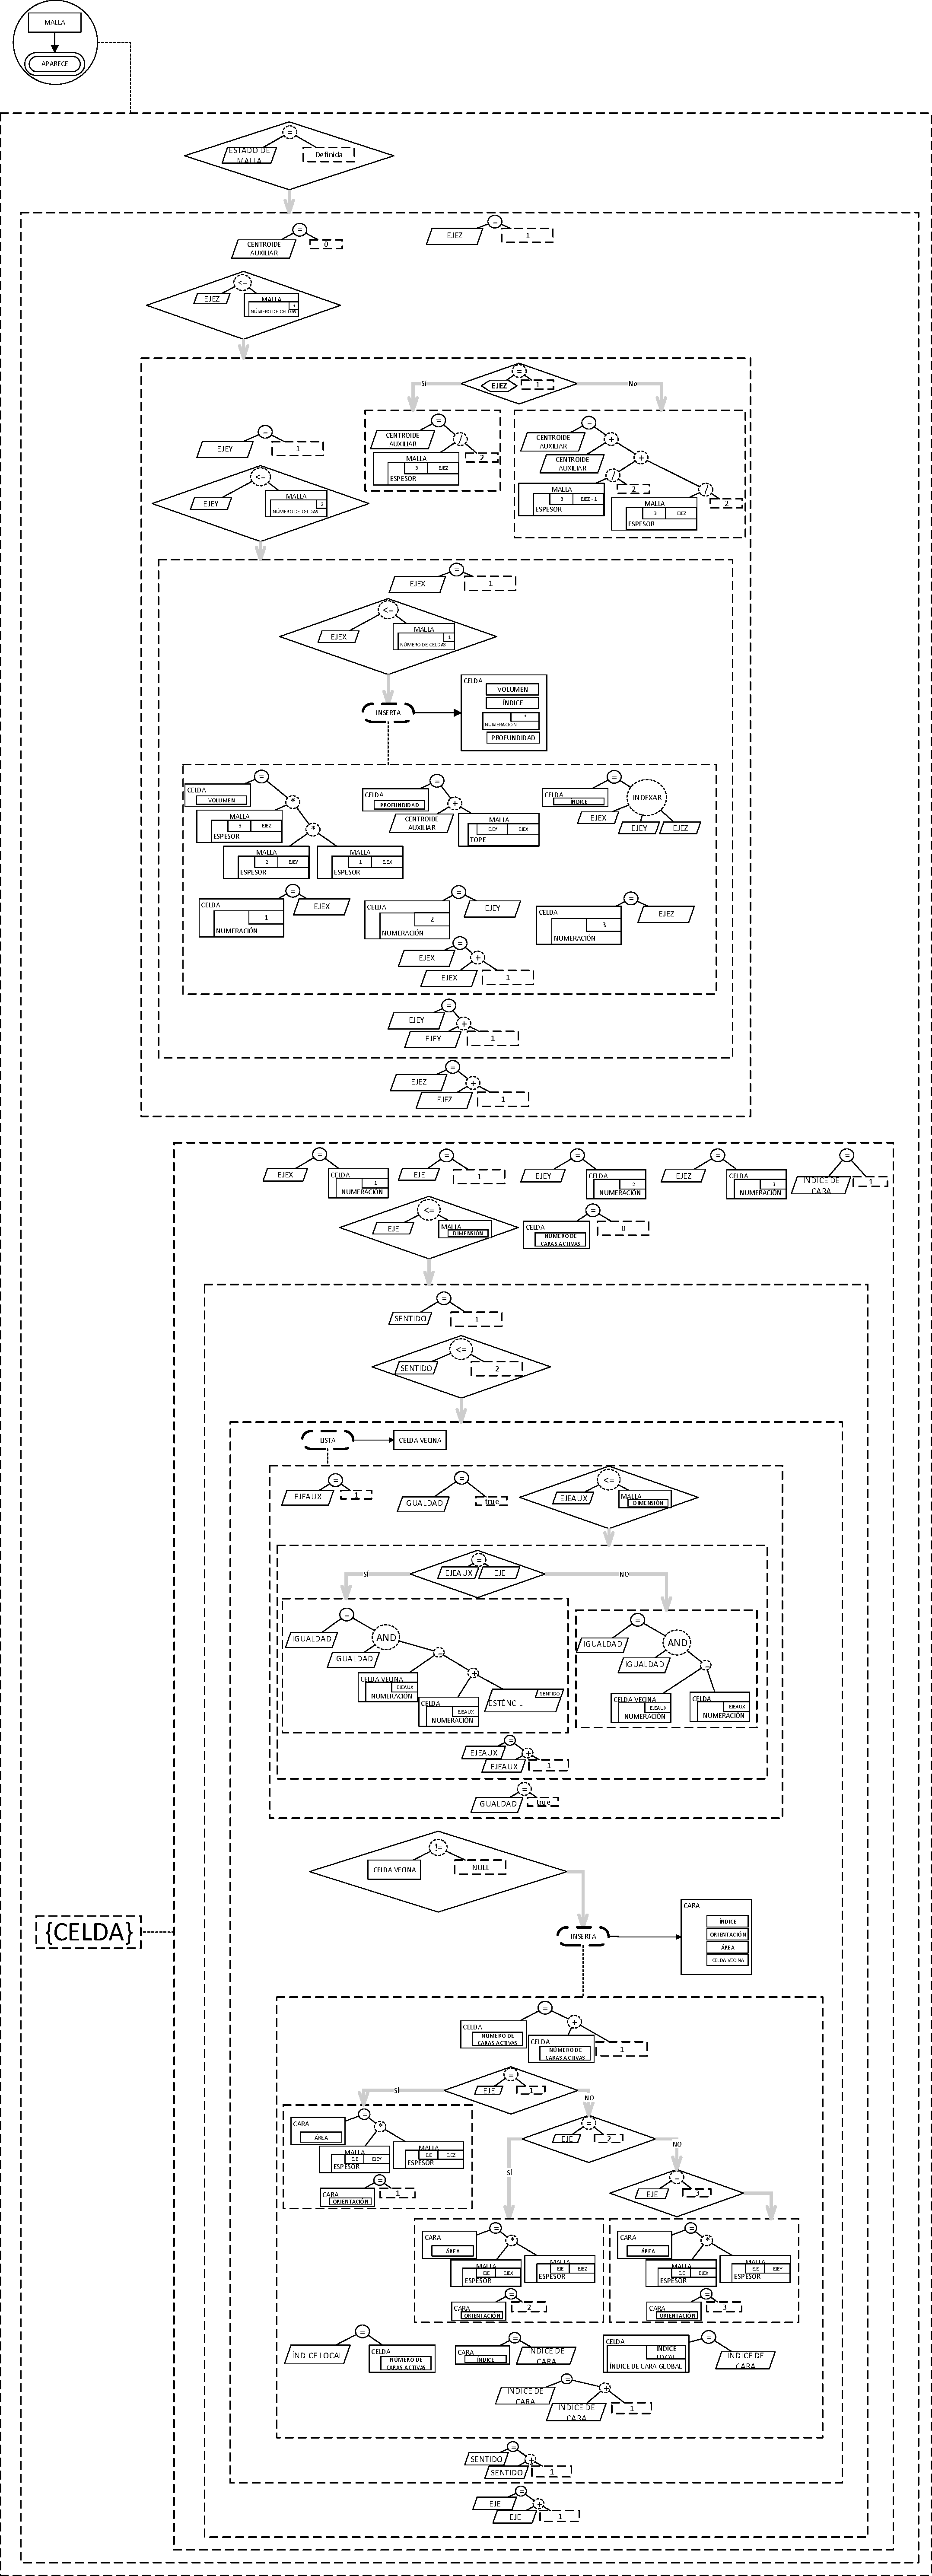
\includegraphics[height=0.9\textheight]{Fig/MallaAparece.pdf}%
	%\caption{Complete PS Representation for EOR Processes} \label{fig:PSComplete}
	\caption[Representación de la aparición de la Malla.]{Representación de la aparición de la Malla. Los autores.} \label{fig:MeshAppears}
\end{figure}

En el segundo ciclo principal, se itera sobre las celdas definidas previamente y se calcula la conectividad, es decir la definición de caras. Para esto, se consulta la existencia de celdas adyacentes a la celda actual en todas las direcciones. Si existe una celda en alguna dirección, se crea y calcula su área y orientación. Adicionalmente, a la cara se le asigna un índice y también se le asigna la celda vecina. Es importante notar que cada celda almacena su conjunto de caras, por lo que las caras se duplican.

\subsection{Tiempo pasa}\label{sec:PS_TimePasses}
El evento ``Tiempo pasa'' se dispara en el momento en que se tiene las suficientes realizaciones de los conceptos para ejecutar la simulación, es decir, se ejecutaron las mínimas relaciones dinámicas para poder disparar el evento, como se ve en la figura \ref{fig:Events}. En este evento se procesa el inicio y el final de la simulación, incrementando el ``tiempo'' y ``término'' al que se van a calcular las propiedades de los conceptos principales.\\

Se puede observar también que, en este evento se realiza el cálculo de las propiedades iniciales para toda la malla. Debido a que, al término cero, sólo se tienen las propiedades que son insertadas en las relaciones dinámicas ejecutadas previamente. las demás propiedades deben ser calculadas como se presenta en la figura \ref{fig:Concepts}, puesto que son necesarias para el término de acumulación en las ecuaciones de transporte para todos los fluidos existentes.

\begin{figure}[h]
	\centering%
	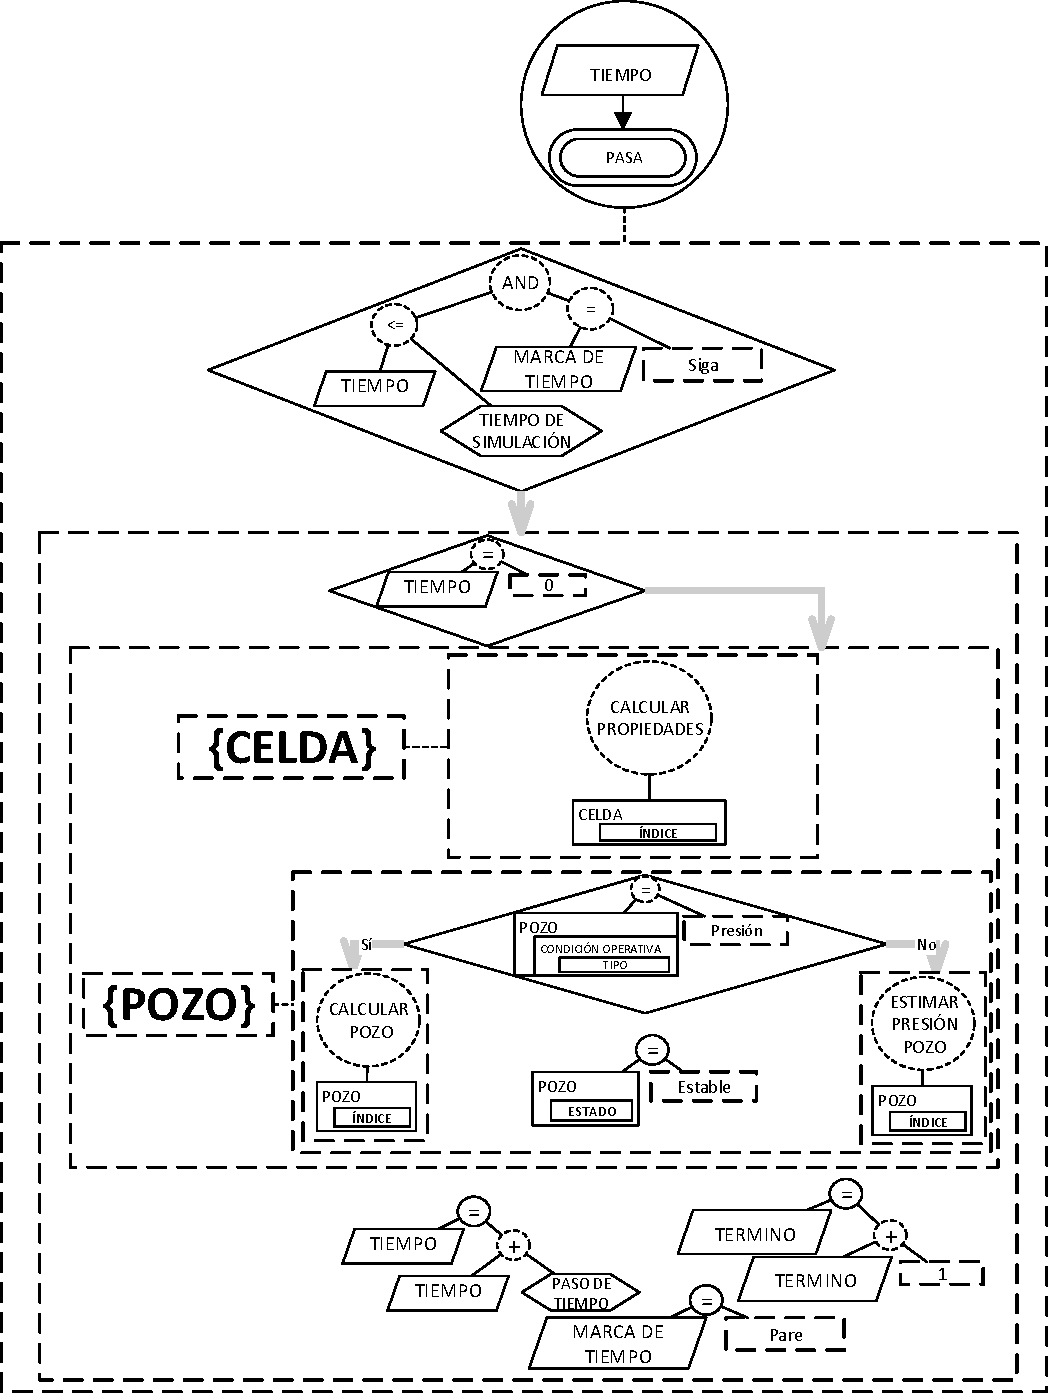
\includegraphics[width=0.7\linewidth]{Fig/TiempoPasa.pdf}%
	%\caption{Complete PS Representation for EOR Processes} \label{fig:PSComplete}
	\caption[Representación del paso del tiempo.]{Representación del paso del tiempo. Los autores.} \label{fig:TimePasses}
\end{figure}


\subsection{Presión del Fluido Varía}\label{sec:PS_FluidVaries}
En el evento ``Presión del Fluido varía'' se procesa el núcleo de la simulación. En éste se llevan a cabo las iteraciones del método de Newton-Raphson para converger al próximo paso de tiempo. La especificación de este evento consta de cinco procesos principales: La actualización de propiedades al término actual, el recálculo de las mismas, el cálculo de los residuales en cada iteración, el cálculo de la matriz jacobiana, y la actualización de las incógnitas. La especificación del evento ``Presión del Fluido varía'' se presenta en la figura \ref{fig:FluidPressureVaries}.\\

\begin{figure}[h]
	\centering%
	\includegraphics[width=0.9\linewidth]{Fig/PresionVaria.pdf}%
	%\caption{Complete PS Representation for EOR Processes} \label{fig:PSComplete}
	\caption[Especificación del evento Presión del fluido varía.]{Especificación del evento Presión del fluido varía. Los autores.} \label{fig:FluidPressureVaries}
\end{figure}

\subsubsection{Actualización de arreglos de propiedades}\label{subsec:PS_DefVars}
En la actualización de propiedades al término actual, se hace un incremento de tamaño y asignación del estimado inicial para el método de Newton-Raphson para todas las celdas de la malla y en todos los fluidos para todas las propiedades dependientes del tiempo. Lo mismo se realiza para los pozos y cada uno de sus perforados. La actualización de propiedades se expone en la figura \ref{fig:UpdateProperties}. 

\begin{figure}[h]
	\centering%
	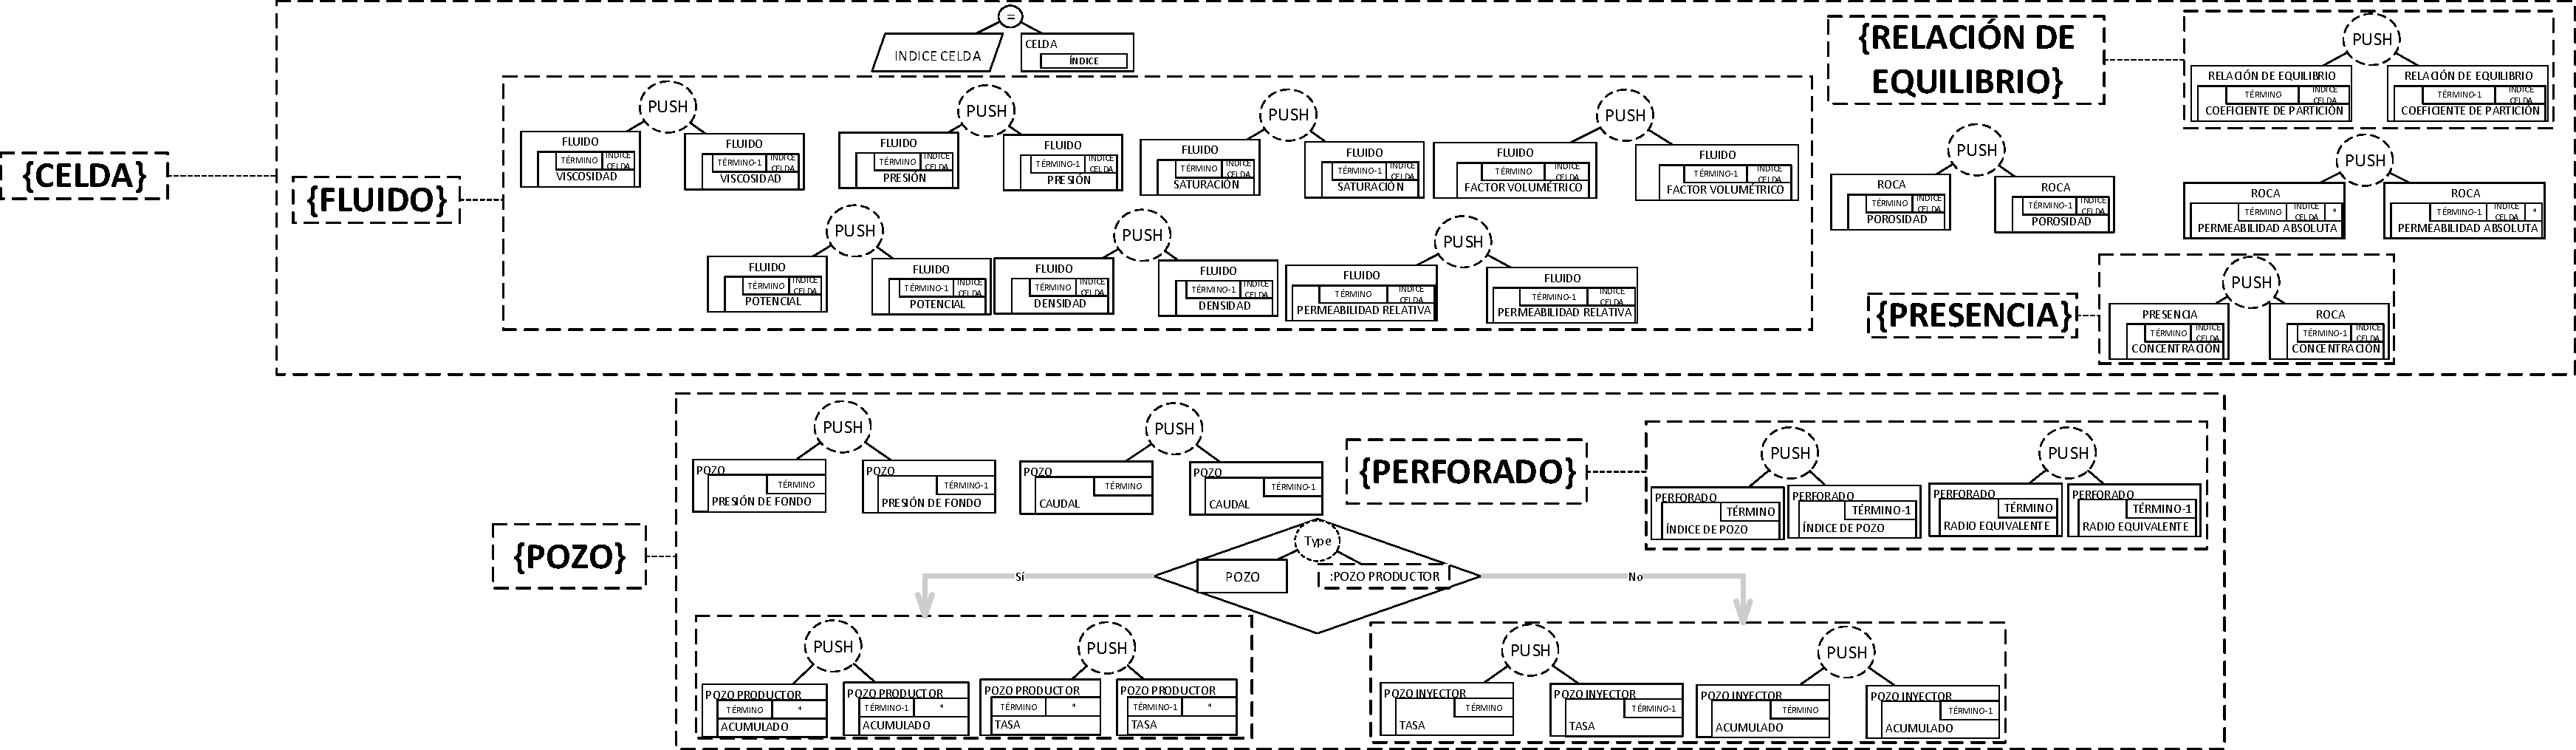
\includegraphics[width=\linewidth]{Fig/ActualizacionDeVariables.pdf}%
	%\caption{Complete PS Representation for EOR Processes} \label{fig:PSComplete}
	\caption[Actualización de propiedades al término actual.]{Actualización de propiedades al término actual. Los autores.} \label{fig:UpdateProperties}
\end{figure}


\subsubsection{Recálculo de propiedades de los fluidos}\label{subsec:PS_TimeK}
Posteriormente en la figura \ref{fig:TimeK} se muestra el recálculo de las propiedades de los fluidos para cada celda. Como el sistema que se resuelve tiene por incógnitas la presión del fluido principal y la saturación de los demás fluidos, es necesario calcular el resto de las propiedades de los fluidos como funciones de estas. \\%Time K

\begin{figure}[h]
	\centering%
	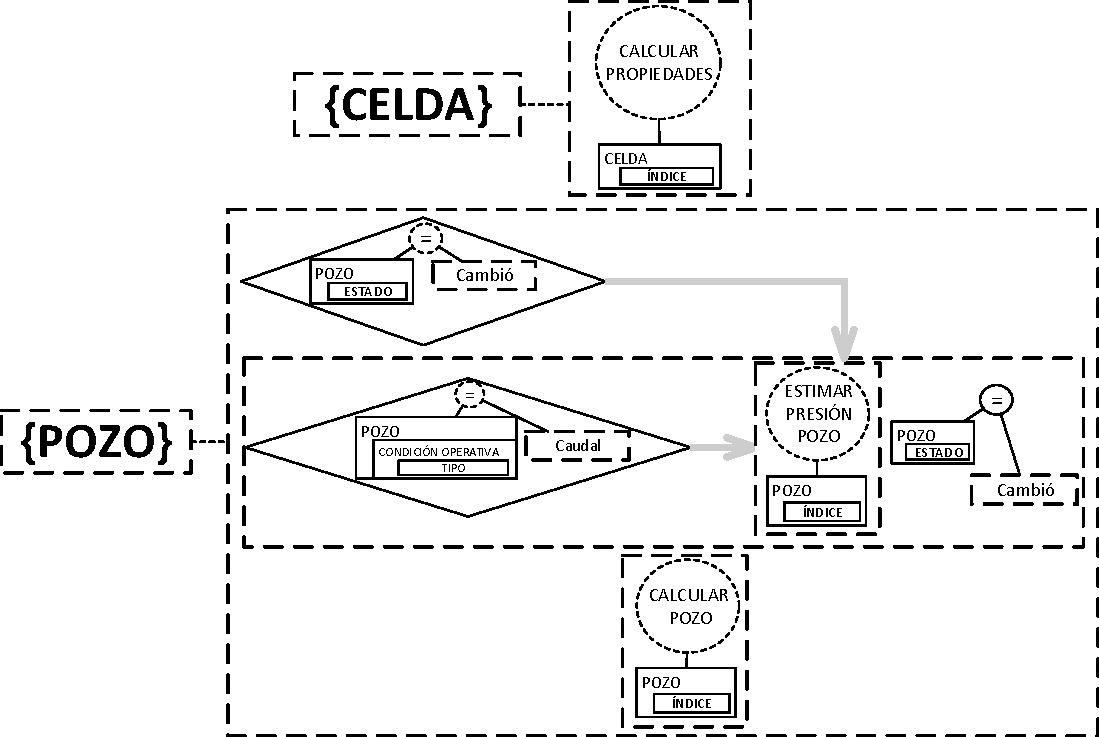
\includegraphics[width=\linewidth]{Fig/TiempoK.pdf}%
	%\caption{Complete PS Representation for EOR Processes} \label{fig:PSComplete}
	\caption[Recálculo de Propiedades al término actual para la iteración.]{Recálculo de Propiedades al término actual para la iteración. Los autores.} \label{fig:TimeK}
\end{figure}

\subsubsection{Cálculo de Residuales}\label{subsec:Residual}
Luego se hace un recorrido de todas las ecuaciones, y se calcula el residual dependiendo de si la ecuación es de tipo fluido o de tipo pozo, cabe aclarar que sólo las ecuaciones de tipo pozo pueden tener como estado "Inactivas".\\

Es importante notar también, que la función ubicar se encarga de calcular la posición correspondiente en el vector residual que agrupa todas las incógnitas a resolver. Además el tipo de residual indica si se debe ubicar como una ecuación de fluido que se evalúa para todas las celdas o sólo es una ecuación de pozo y por tanto una sola fila en las últimas posiciones del residual, tal comportamiento se evidencia en \ref{fig:Residual}. \\ % Residual

\begin{figure}[h]
	\centering%
	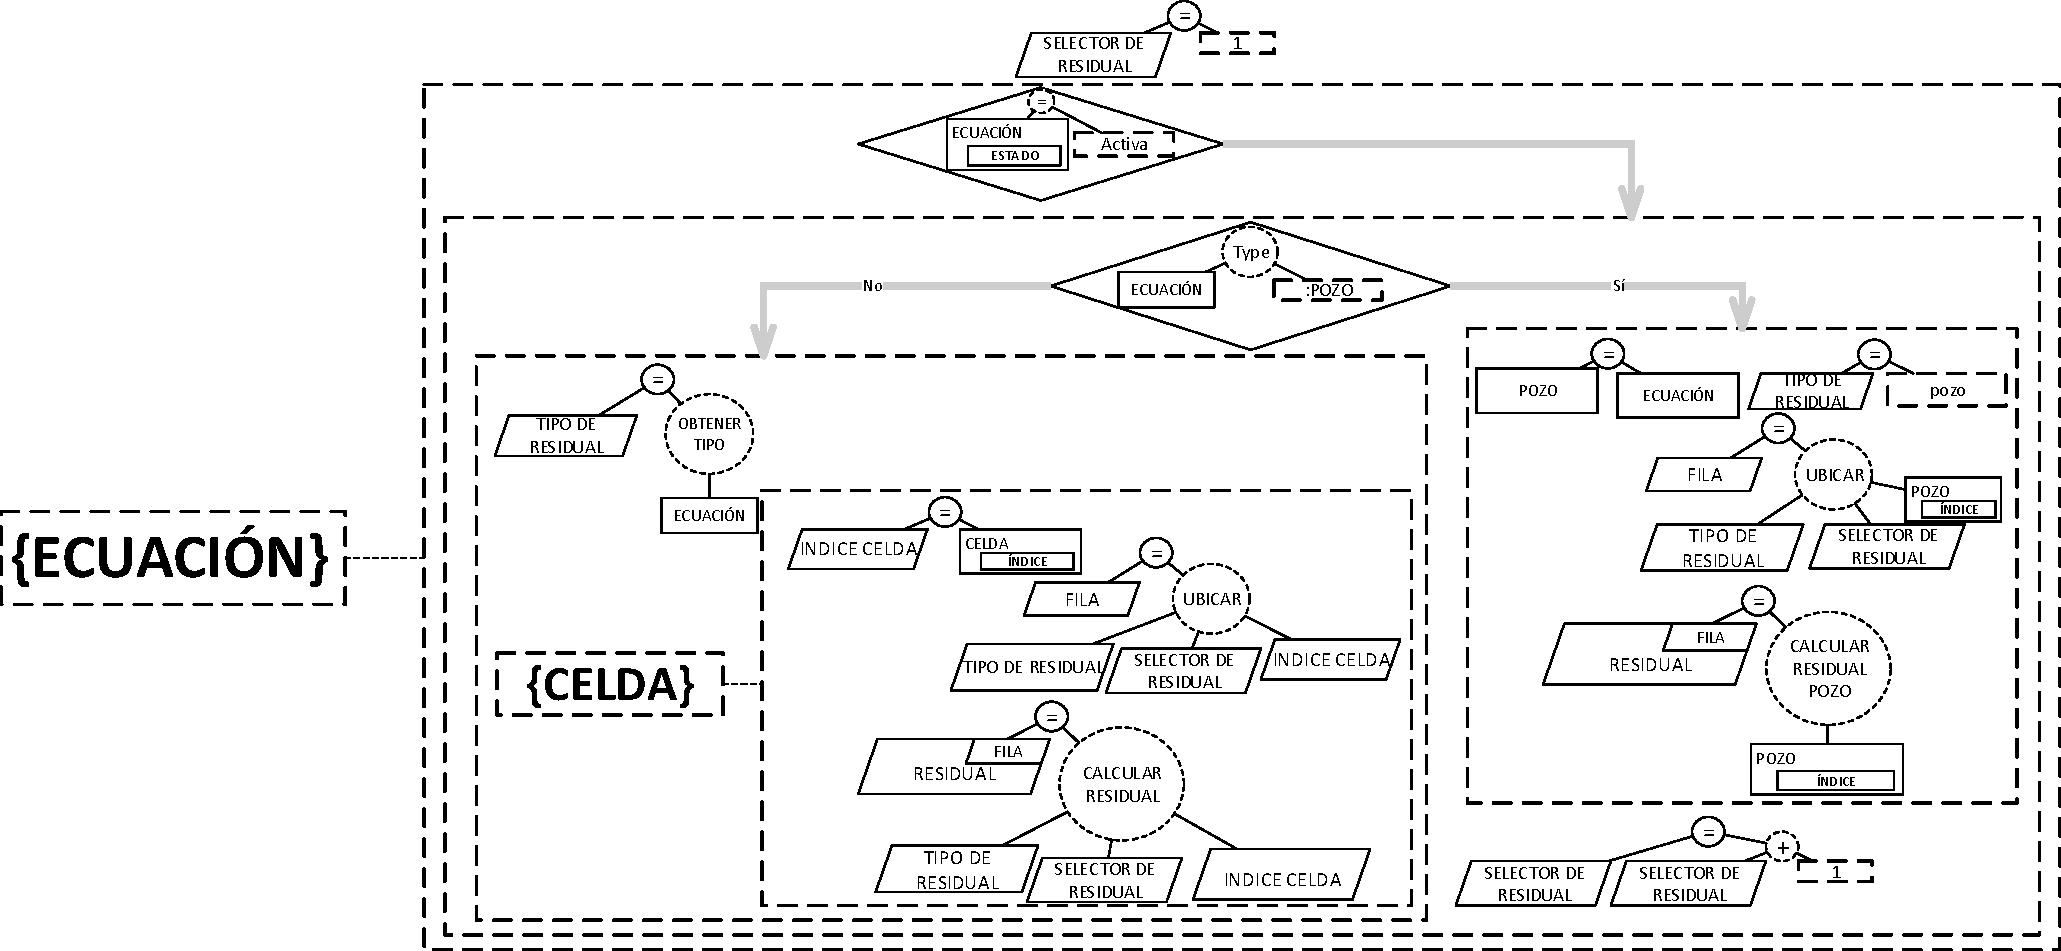
\includegraphics[width=\linewidth]{Fig/Residual.pdf}%
	%\caption{Complete PS Representation for EOR Processes} \label{fig:PSComplete}
	\caption[Cálculo de residual para la iteración.]{Cálculo de residual para la iteración. Los autores.} \label{fig:Residual}
\end{figure}

\subsubsection{Cálculo de la Matriz del Jacobiano}\label{subsec:Jacobian}
Siguiendo \ref{fig:Jacobiano} \\ % Jacobiano

\begin{figure}[h]
	\centering%
	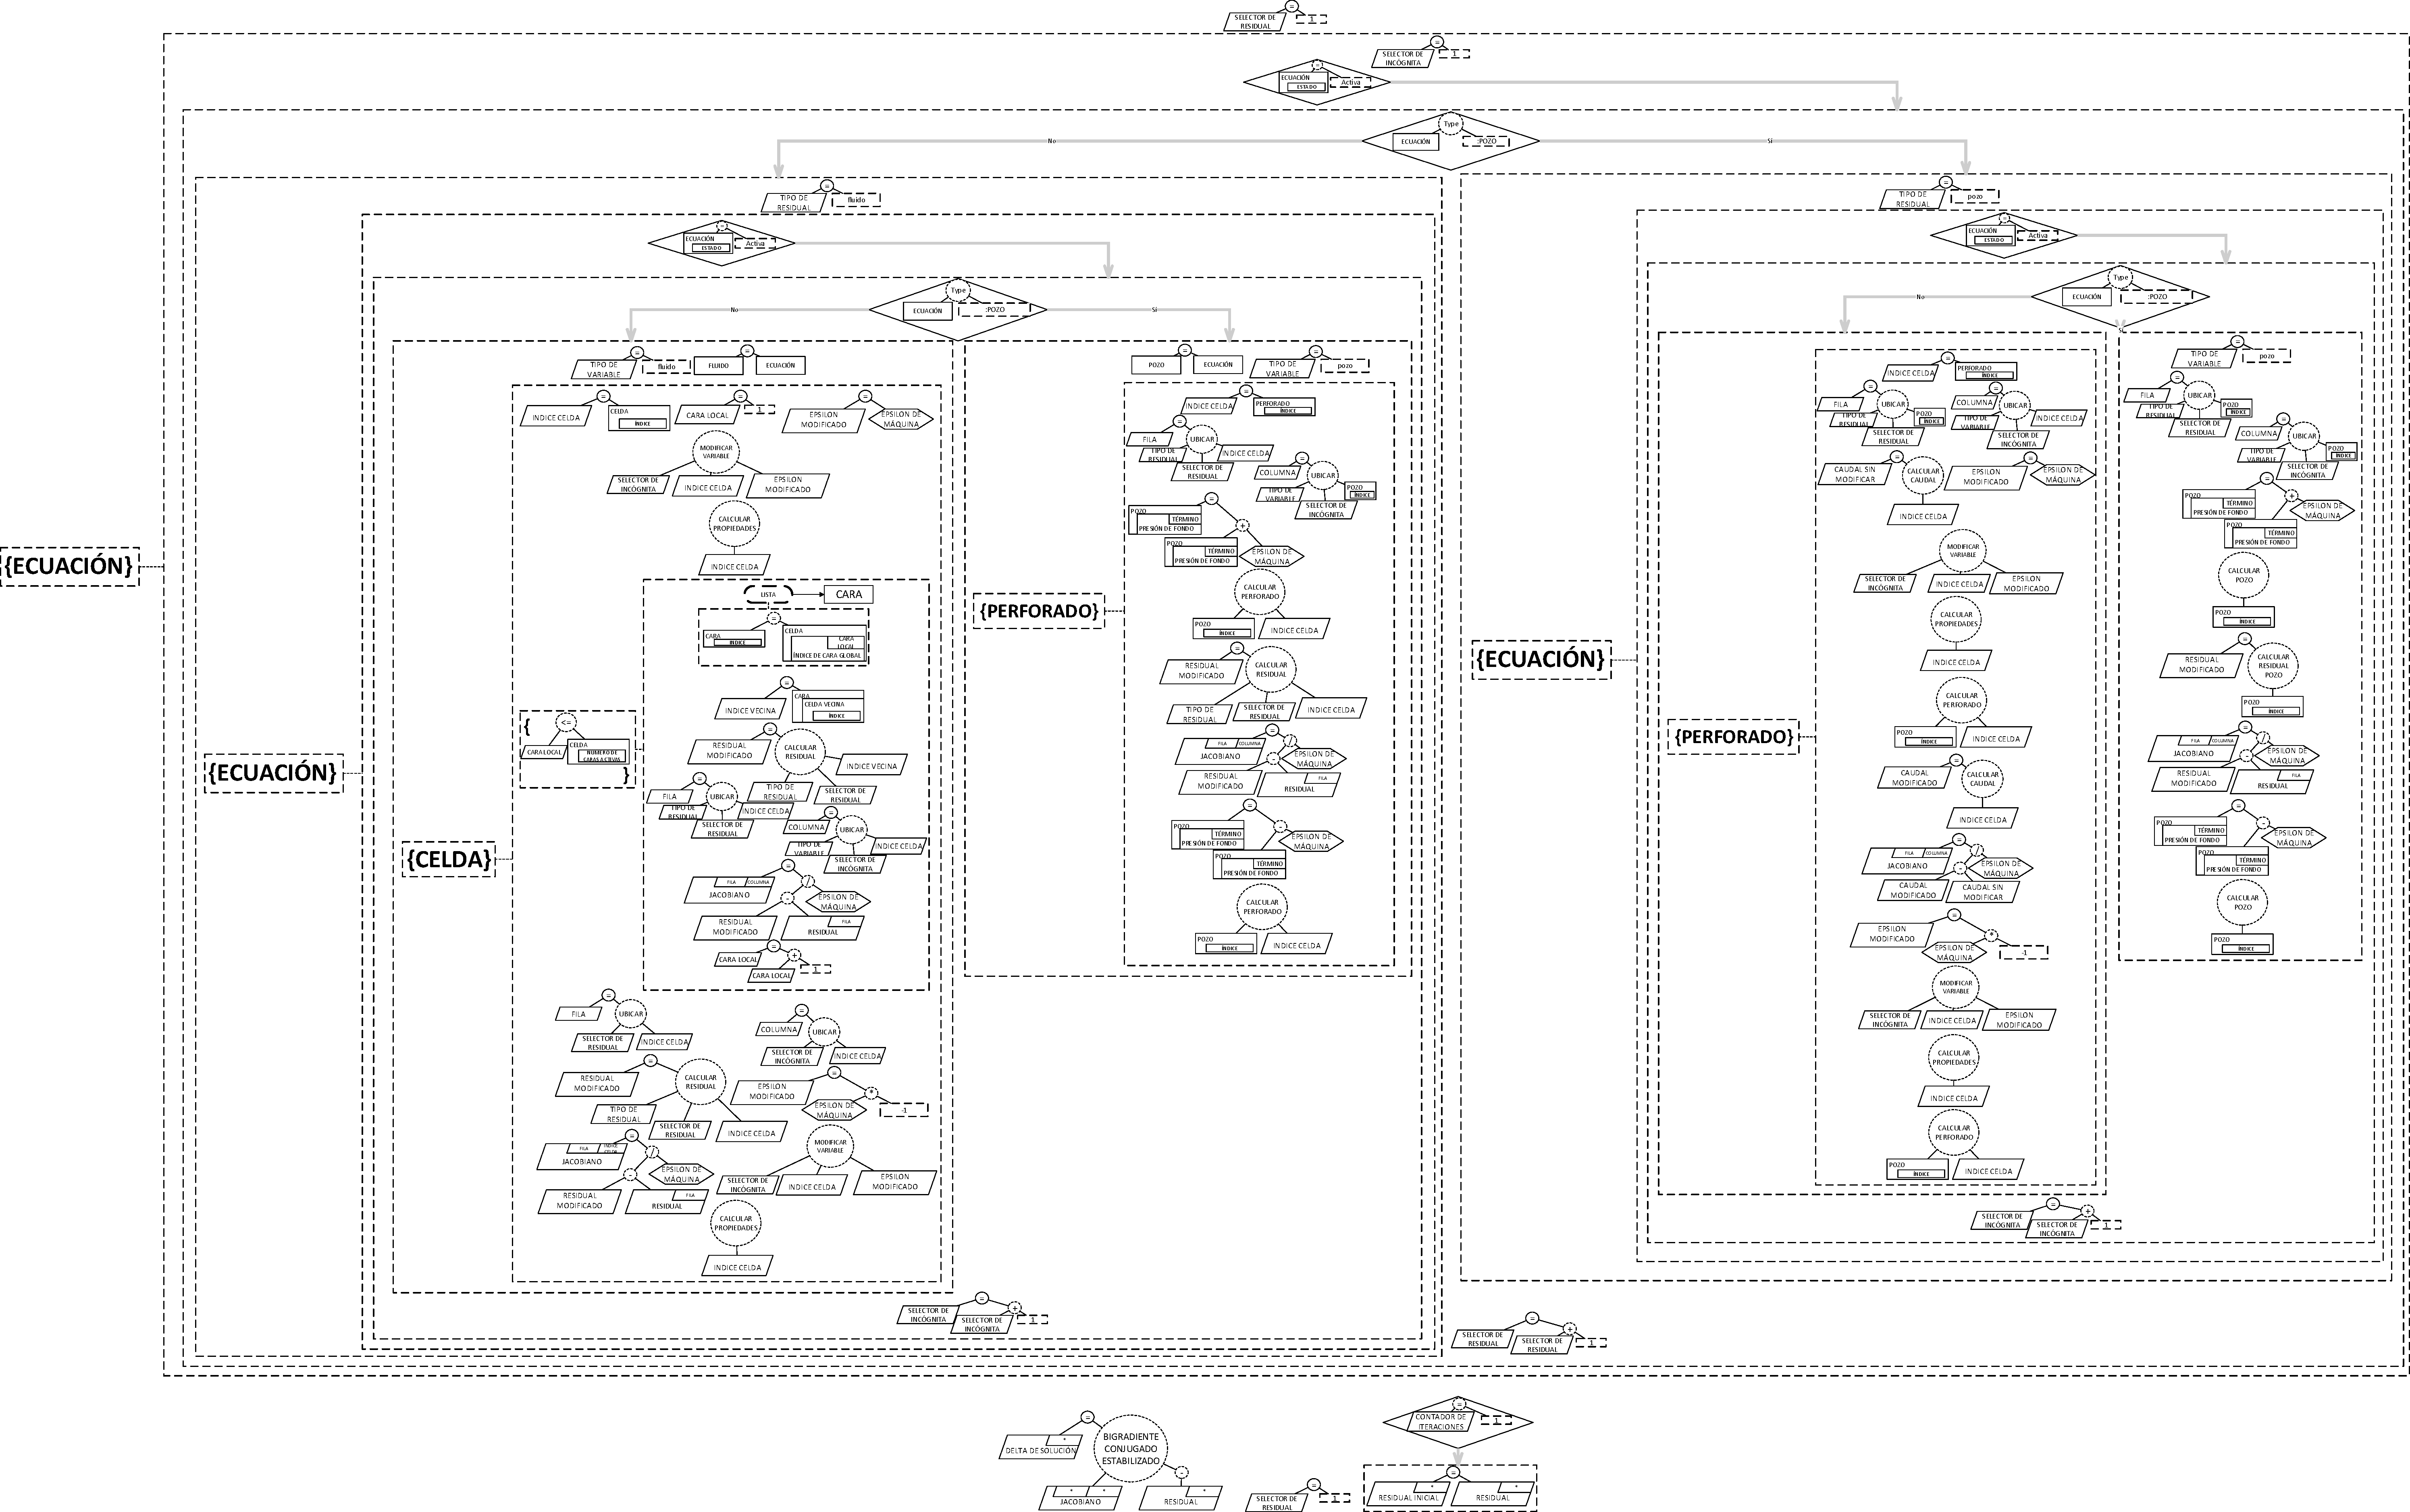
\includegraphics[width=\linewidth]{Fig/Jacobiano.pdf}%
	%\caption{Complete PS Representation for EOR Processes} \label{fig:PSComplete}
	\caption[Cálculo y armado de la matriz del jacobiano al término actual para la iteración.]{Cálculo y armado de la matriz del jacobiano al término actual para la iteración. Los autores.} \label{fig:Jacobiano}
\end{figure}

\subsubsection{Solución del sistema lineal y actualización de incógnitas}
Por último una vez se tiene la matriz del jacobiano construida se soluciona usando el operador ``Bigradiente conjugado estabilizado", proveniente de alguna librería, que resuelve el sistema: $Jacobiano*DeltaDeSolucion = -Residual$ como se observa en \ref{fig:LinearSystem}. Posteriormente, se actualizan las incógnitas sumándoles el delta de solución de manera acorde al cálculo del residual. Esto se presenta en \ref{fig:UpdateVariables}. \\

\begin{figure}[h]
	\centering%
	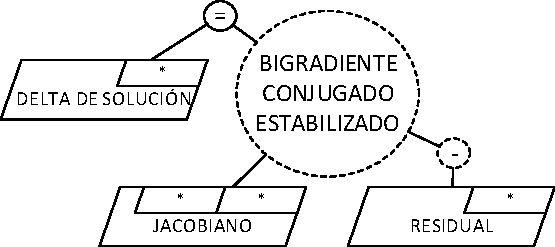
\includegraphics[scale=1]{Fig/SistemaLineal.pdf}%
	%\caption{Complete PS Representation for EOR Processes} \label{fig:PSComplete}
	\caption[Sistema lineal resultante del método de Newton-Raphson.]{Sistema lineal resultante del método de Newton-Raphson. Los autores.} \label{fig:LinearSystem}
\end{figure}

\begin{figure}[h]
	\centering%
	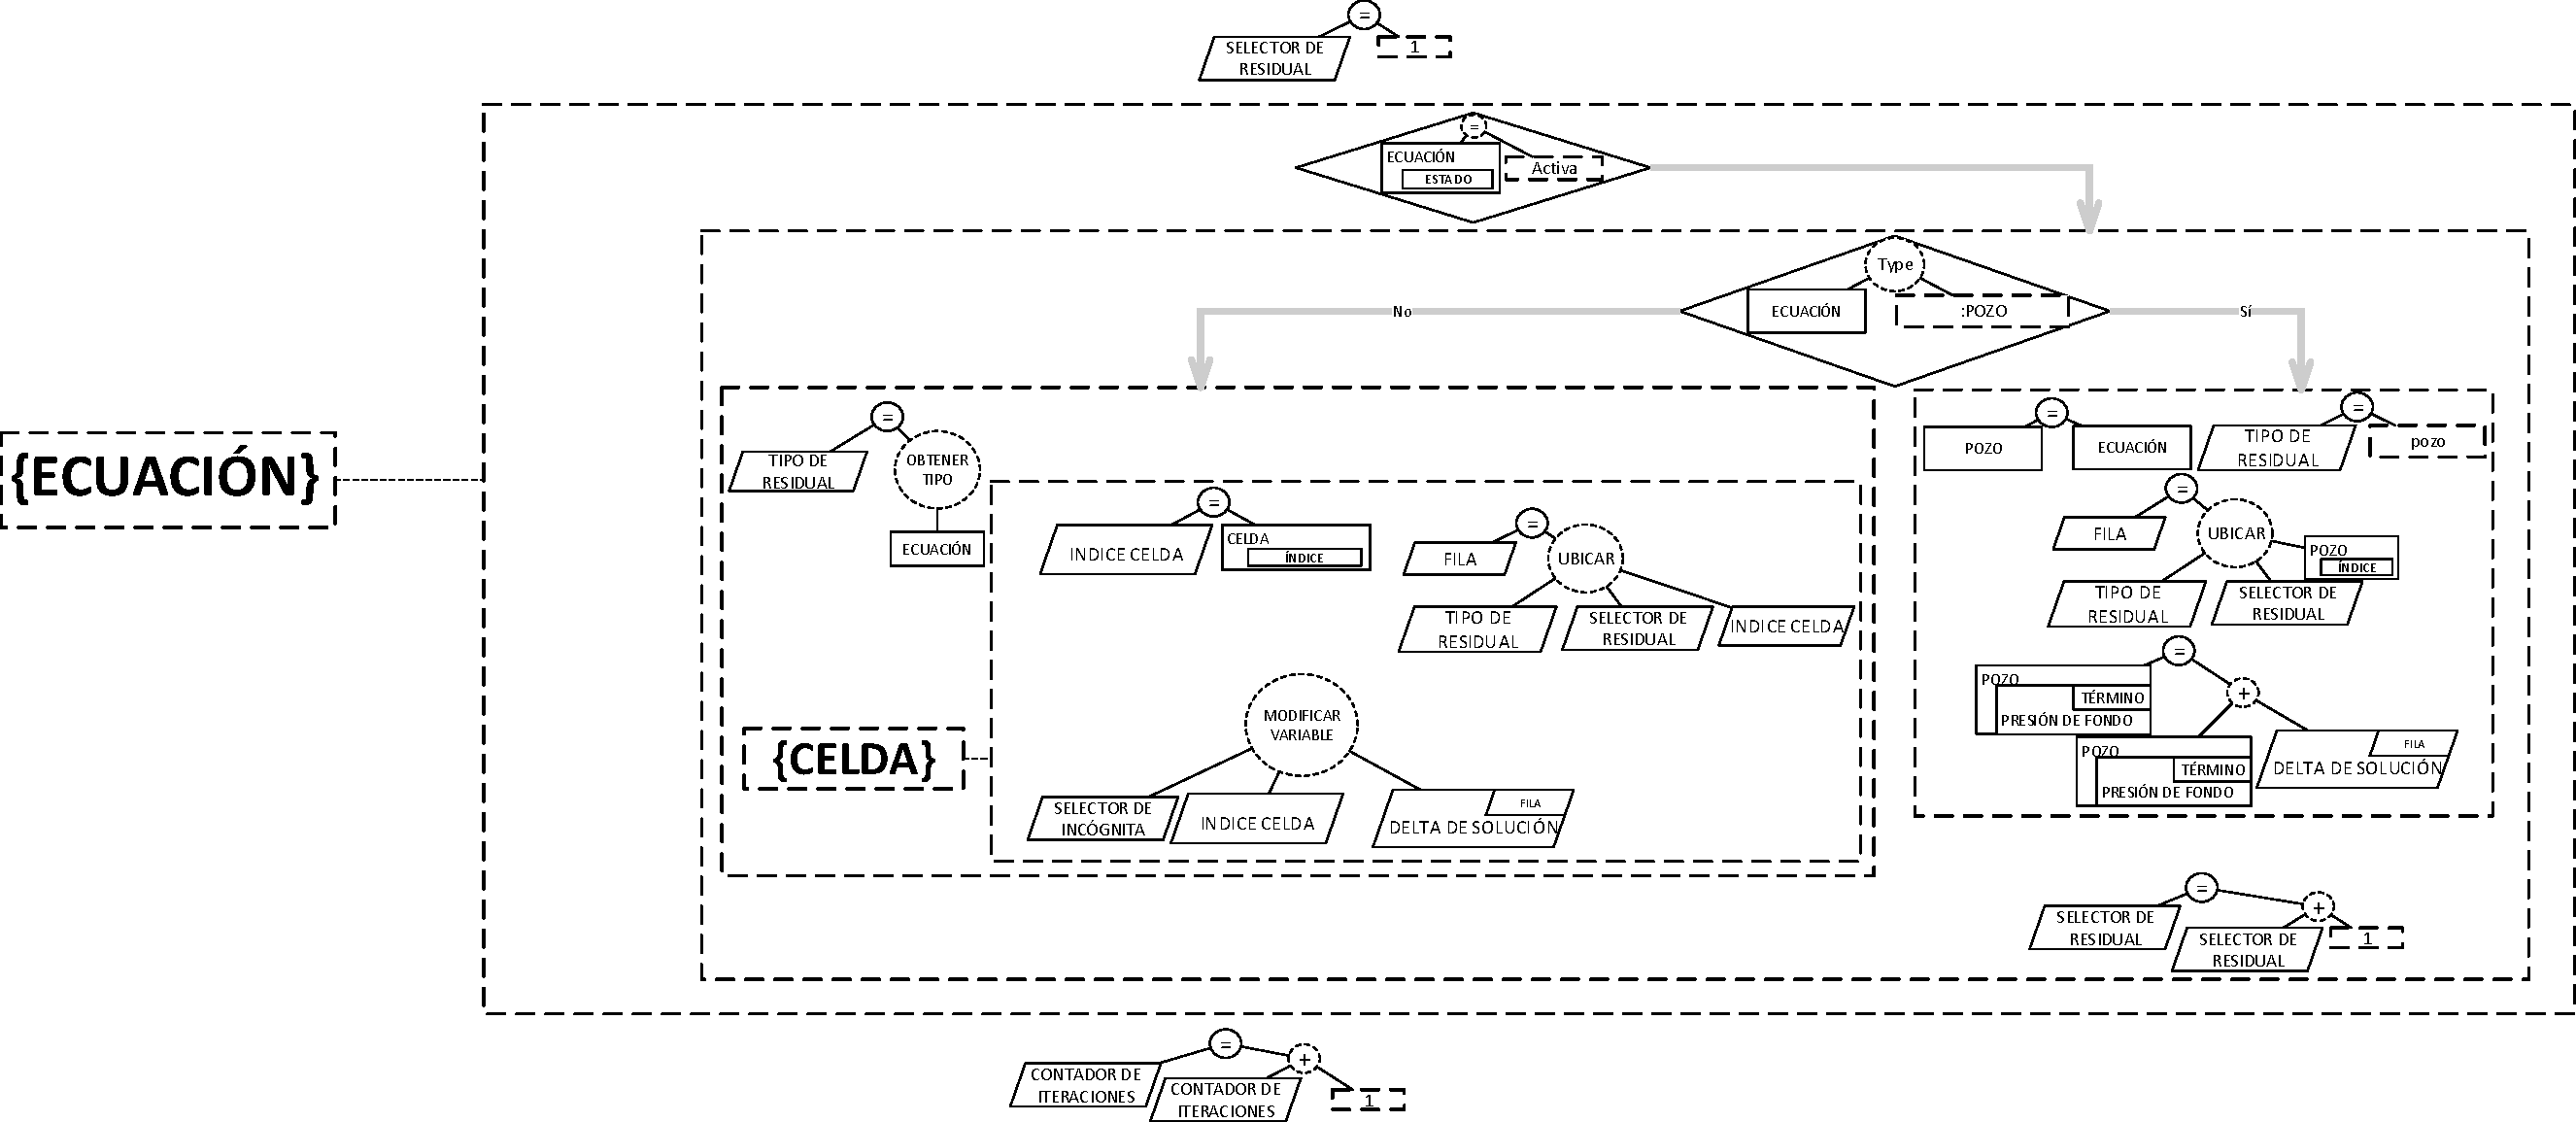
\includegraphics[width=\linewidth]{Fig/ActualizacionDeIncognitas.pdf}%
	%\caption{Complete PS Representation for EOR Processes} \label{fig:PSComplete}
	\caption[Recálculo de Propiedades al término actual para la iteración.]{Recálculo de Propiedades al término actual para la iteración. Los autores.} \label{fig:UpdateVariables}
\end{figure}
%includefigure{Graphical Representation of subroutine}

%includegraphic{Code Translation}

%Se deben incluir tantos cap\'{\i}tulos como se requieran; sin embargo, se recomienda que la tesis  o trabajo de investigaci\'{o}n tenga un m\'{\i}nimo 3 cap\'{\i}tulos y m\'{a}ximo de 6 cap\'{\i}tulos (incluyendo las conclusiones).\\
\chapter{Validación y Resultados}\label{cap:Validacion}
%Se deben incluir tantos cap\'{\i}tulos como se requieran; sin embargo, se recomienda que la tesis  o trabajo de investigaci\'{o}n tenga un m\'{\i}nimo 3 cap\'{\i}tulos y m\'{a}ximo de 6 cap\'{\i}tulos (incluyendo las conclusiones).\\

%\renewcommand{\tablename}{\textbf{Código}}
\section{Traducción a Código}
En esta Sección se muestran porciones del modelo ejecutable que se programa en C++ \citep{ISO:2017:IIIa}. Se elije este lenguaje porque la \textit{Stardard Template Library} (STL) tiene facilidades que permiten hacer explícita la consistencia del código con el esquema preconceptual. Se emula una base de datos a partir de arreglos globales que almacenan cada concepto, y, las claves foráneas que se generan entre conceptos se traducen como punteros. \\

A continuación se muestra, a modo de ejemplo, las traducciones de algunos conceptos, funciones, o porciones del EP a código C++ para verificar la consistencia del código con el modelo ejecutable. Primero, se definen los elementos que conforman las condiciones iniciales, y, la base de datos que se emula, es decir, los arreglos que contienen los conceptos que se instancian en la ejecución de las relaciones dinámicas del EP. Posteriormente, se muestran las traducciones a código de dos conceptos clase, ``Malla'' y ``Roca'', y la traducción de la relación dinámica ``Petrofísico caracteriza Roca''. Luego, se explica la traducción del cálculo del residual en el evento ``Presión del Fluido Varía''.\\

Las condiciones iniciales, en las que se definen variables globales y constantes, se programan en un \textit{namespace} ``Global'' que agrupa todas las definiciones, tal como aparecen en la figura \ref{fig:EjInitialConditions}. El código para las condiciones iniciales se expone en la Tabla \ref{tab:InitialConditions}.\\

\begin{table}[h!]
	\centering
	\begin{tabular}{cc}
		\parbox[c]{10em}{
			\begin{tabular}[c]{@{}c@{}}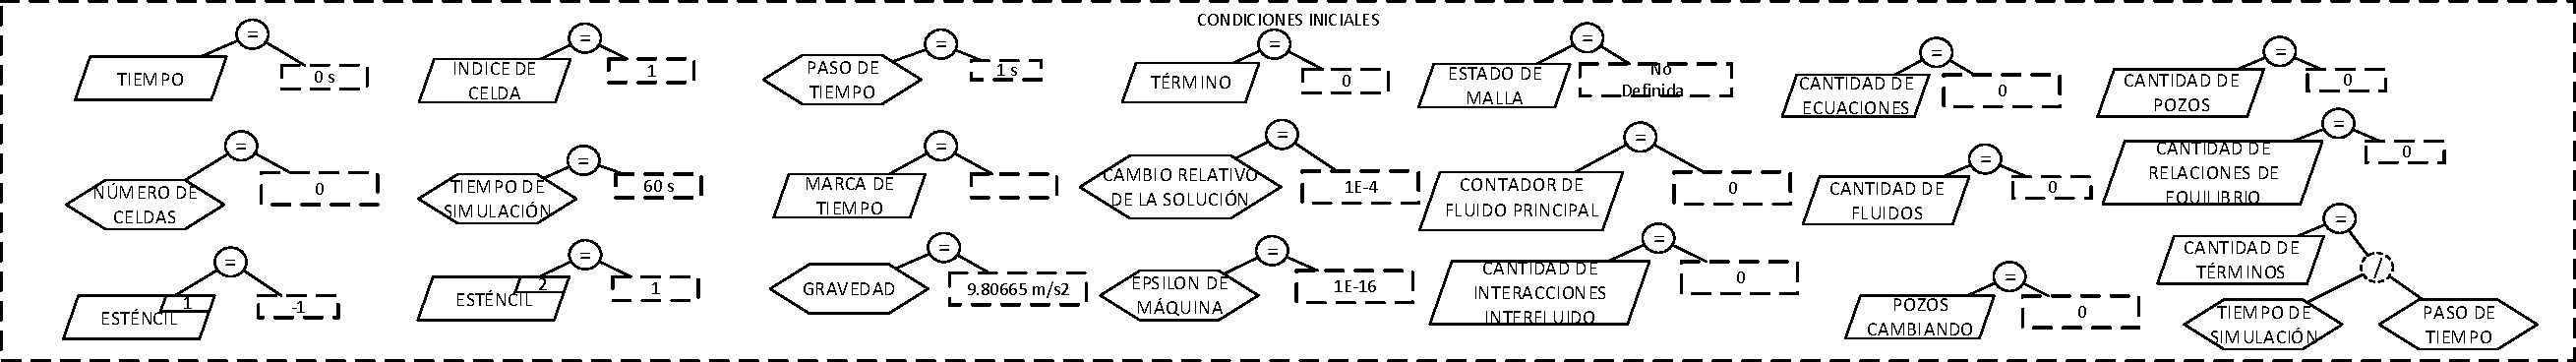
\includegraphics[width=3in]{Fig/EjInitialConditions.pdf}\\ Ver figura \ref{fig:EjInitialConditions}.\end{tabular}
			%
			%\caption[Elementos para la representación de Software Científico.]{Elementos para la representación de Software Científico. \citep{JCalle,norena2018det}.} \label{fig:RockTranslation}
		}
		&
		\begin{tiny}
			\begin{lstlisting}
			namespace Initial_Conditions{
			
			std::string timestamp="";
			double mytime=0;
			double simulationtime = 86400;
			double timedelta=1;
			int wells_quantity=0;
			int term=0;
			int fluids_quantity=0;
			int stencil[2] = {-1,1};
			int equilibrium_relations_quantity=0;
			int interfluid_interactions_quantity=0;
			int cells_number=0;
			int changing_wells=0;
			
			};
			
			\end{lstlisting}
		\end{tiny}
	\end{tabular}
	\caption[Traducción a código de las condiciones iniciales.]{Traducción a código de las condiciones iniciales. Los autores. \label{tab:InitialConditions}}
\end{table}

En el código de la Tabla \ref{tab:bd} se muestran los conceptos que se almacenan en arreglos, estos se iteran en diferentes funciones del código. Es importante notar que, en las precondiciones del EP se establece que sólo se define una única malla y sólo se caracteriza una única roca. Por tanto, en la base de datos que se emula, estos dos conceptos se acceden por medio de un puntero único. También se destaca que, todos los objetos que se instancian de los conceptos clase, se acceden a partir de punteros. Todos los punteros se fundamentan en la STL, que se encarga de hacer la respectiva gestión del uso de la memoria.\\

\begin{table}[h!]
	\begin{tabular}{c}
		\begin{tiny}
			\begin{lstlisting}
			
			std::vector<std::shared_ptr<Equation_Base>> equations =
			std::vector<std::shared_ptr<Equation_Base>>();
			
			std::vector<std::shared_ptr<Fluid>> characterized_fluids =
			std::vector<std::shared_ptr<Fluid>>();
			
			std::vector<std::unique_ptr<Equilibrium_Relation>> added_equilibrium_relations =
			std::vector<std::unique_ptr<Equilibrium_Relation>>();
			
			std::vector<std::unique_ptr<Interfluid_Interaction>> added_interfluid_interactions =
			std::vector<std::unique_ptr<Interfluid_Interaction>>();
			
			std::vector<std::shared_ptr<Well>> perforated_wells =
			std::vector<std::shared_ptr<Well>>();
			
			std::unique_ptr<Mesh> mymesh;
			std::unique_ptr<Rock> myrock;
			
			\end{lstlisting}
		\end{tiny}
	\end{tabular}
	\caption[Arreglos que conforman la base de datos que se emula.]{Arreglos que conforman la base de datos que se emula. Los autores. \label{tab:bd}}
\end{table}

En el código de la Tabla \ref{tab:MeshCode} se puede observar que, la conceptualización de la malla coincide con el código que se genera para la misma. La malla se propone como un conjunto de celdas. Adicionalmente, se tienen elementos como el espesor que dependen de la cantidad de celdas en cada dirección. Las celdas también se iteran, pero su arreglo correspondiente se almacena dentro del concepto malla, tal como se propone en la sección \ref{subsec:PS_Mesh}.\\

\begin{table}[h!]
	\centering
	\begin{tabular}{cc}
		\parbox[c]{5em}{
			\begin{tabular}[c]{@{}c@{}}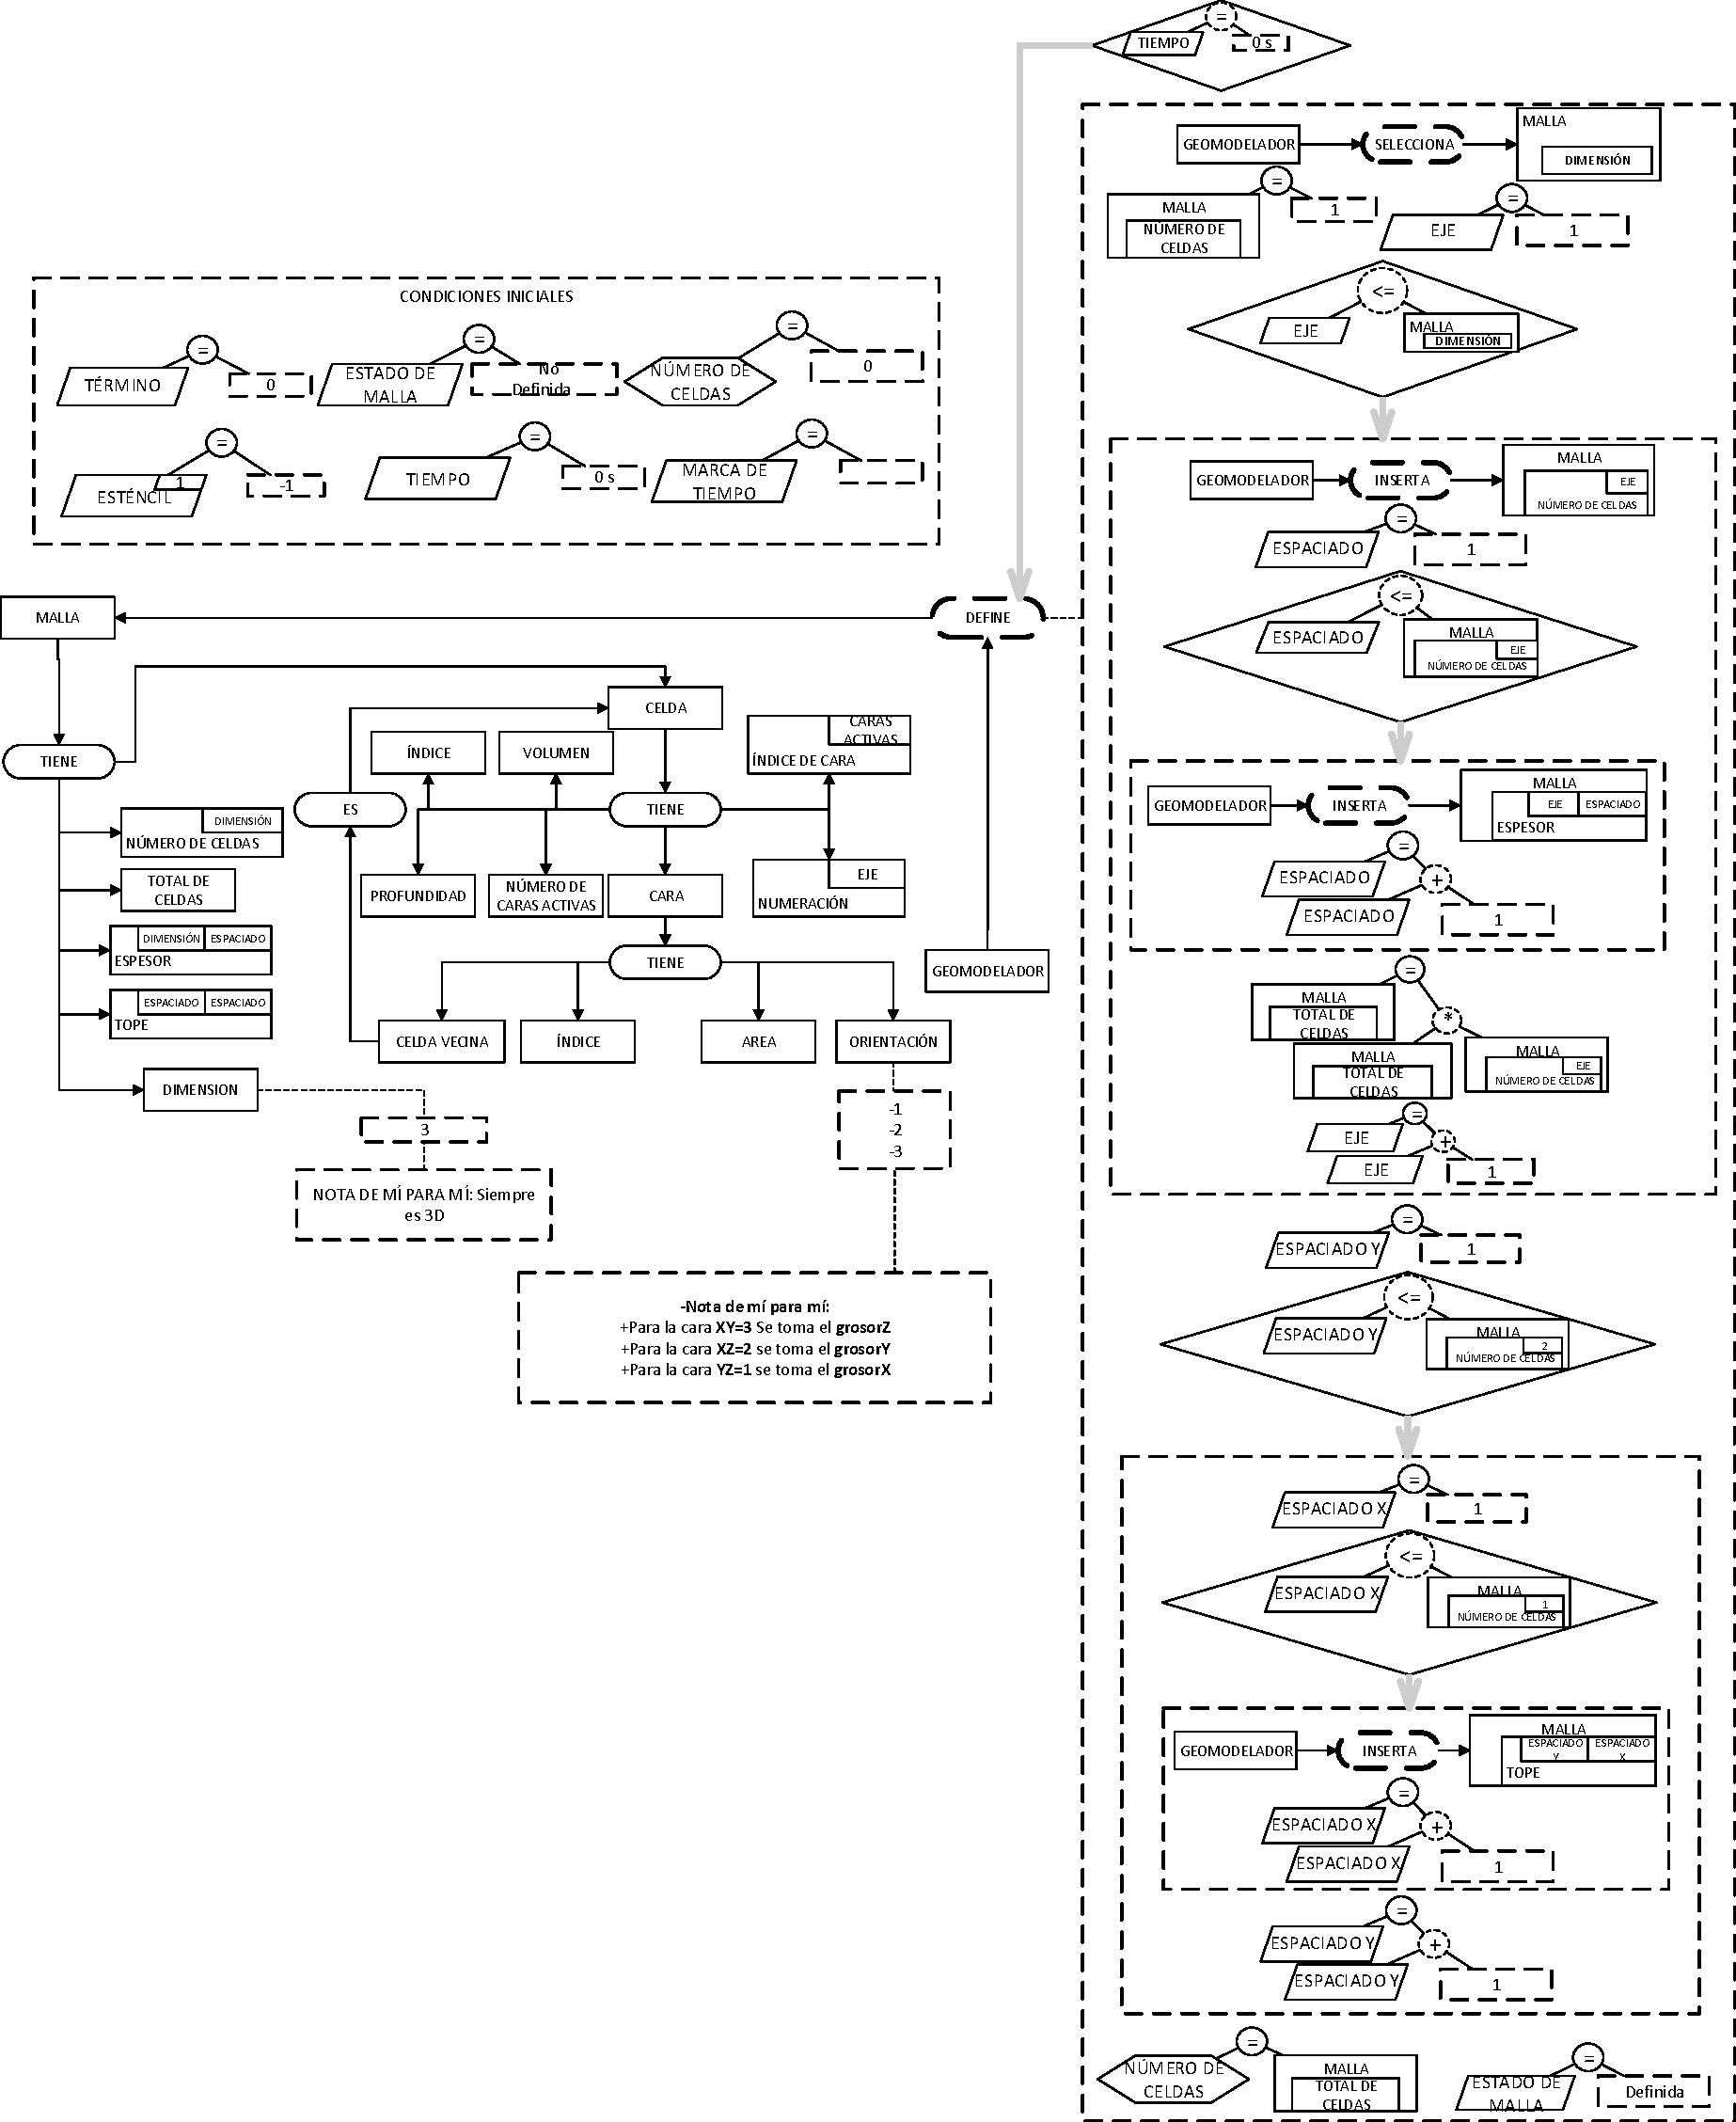
\includegraphics[width=2in]{Fig/Mesh.pdf}\\ Ver figura \ref{fig:Mesh}.\end{tabular}
			%
			%\caption[Elementos para la representación de Software Científico.]{Elementos para la representación de Software Científico. \citep{JCalle,norena2018det}.} \label{fig:RockTranslation}
		}
		&
		\begin{tiny}
			\begin{lstlisting}
			
			class Mesh{
			
			private:
			
			using Cells_t = std::vector<std::shared_ptr<Cell>>;
			int _dimension;
			std::vector<int> _cell_number = std::vector<int>(3);
			int _cell_total;
			std::vector<std::vector<double>> _thickness;
			std::vector<std::vector<double>> _top;
			int _defined=0;
			Cells_t _cells;
			
			public:
			
			using Cell_iterator = Cells_t::iterator;
			using Cell_const_iterator = Cells_t::const_iterator;
			
			Mesh();
			int getCellTotal();
			void define();
			void defineFromFile(std::ifstream& mesh_reader);
			void appear(const std::string& _timestamp, const int stencil[2]);
			
			int listCell(int posx, int posy, int posz);
			int listCell(std::vector<int> _Numeration);
			
			const std::shared_ptr<Cell>& cell(const int index) const 
			{return _cells[index];};
			
			const double& thickness(const int axis, const int spacing) const 
			{return _thickness[axis][spacing];};
			
			Cell_iterator begin() {return _cells.begin();};
			Cell_iterator end()   {return _cells.end();};
			
			Cell_const_iterator begin()  const {return _cells.begin();};
			Cell_const_iterator end()    const {return _cells.end();};
			Cell_const_iterator cbegin() const {return _cells.cbegin();};
			Cell_const_iterator cend()   const {return _cells.cend();};
			
			
			};
			
			\end{lstlisting}
		\end{tiny}
	\end{tabular}
	\caption[Traducción a código del concepto Malla.]{Traducción a código del concepto Malla. Los autores. \label{tab:MeshCode}}
\end{table}

\newpage

En el código de la Tabla \ref{tab:RockCode}, se muestra la definición de la clase Roca, que corresponde al concepto roca en el EP y se pueden notar adicionalmente, la implementación de los \textit{get} y \textit{set} para cada atributo o concepto hoja. En el código de la Tabla \ref{tab:RockCharacterizeCode} se muestra la implementación de la relación dinámica ``petrofísico caracteriza roca''. Ésta se implementa como lecturas por consola, la cuál se desarrolla de manera segura en la función \textit{myRead}. Se logra evidenciar la consistencia en los nombres de los atributos, parámetros y las variables independientes que se definen en la lectura. Adicionalmente, por las dimensiones de los casos que se simulan, se implementa una lectura equivalente usando archivos para mayor facilidad de uso.

\begin{table}[h!]
	\centering
	\begin{tabular}{cc}
		\parbox[c]{1em}{
			\begin{tabular}[c]{@{}c@{}}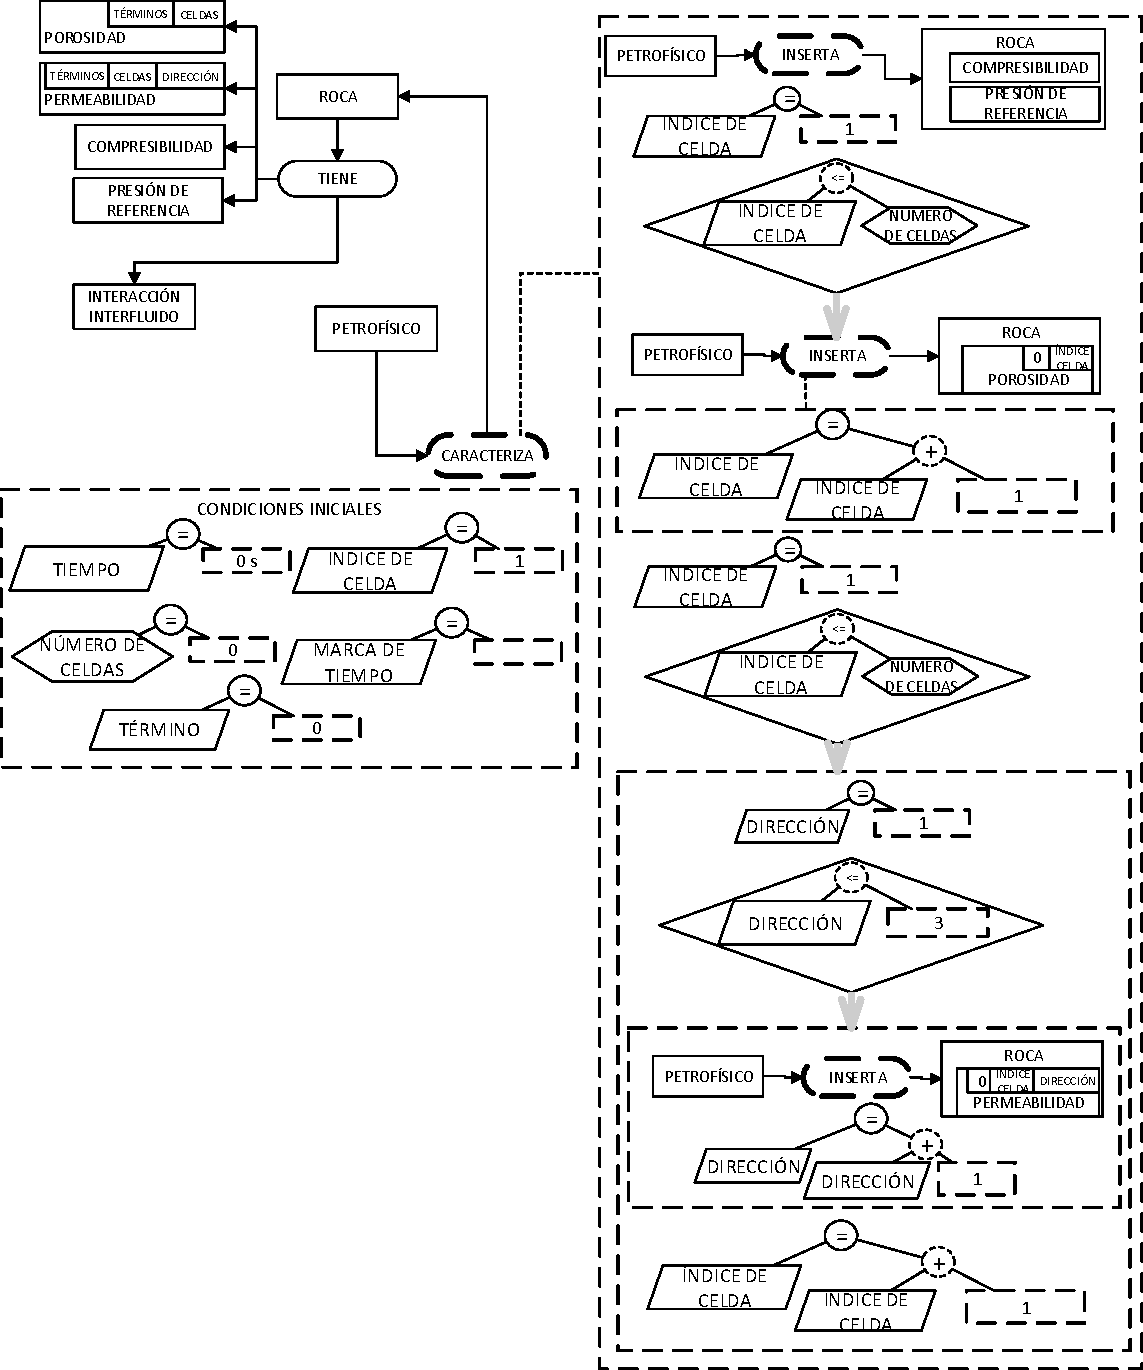
\includegraphics[width=1in]{Fig/Rock.pdf}\\ Ver figura \ref{fig:Rock}.\end{tabular}
			%
			%\caption[Elementos para la representación de Software Científico.]{Elementos para la representación de Software Científico. \citep{JCalle,norena2018det}.} \label{fig:RockTranslation}
		}
		&
		\begin{tiny}
			\begin{lstlisting}
			class Rock{
			private:
			
			double _reference_pressure;
			double _compressibility;
			std::vector<std::vector<std::vector<double>>> _absolute_permeability;   
			std::vector<std::vector<double>> _porosity;
			
			public:
			
			Rock(){};
			void characterize(const int& cells_number);
			void characterizeFromFile(std::ifstream& rock_reader,
			const int& cells_number);
			void porosity(const int term, const int cell_index,
			const double pressure);
			
			void updateProperties(const int& term);
			
			const double& porosity (const int term, const int cells_number) const {
			return _porosity[term][cells_number];
			};
			
			const std::vector<double>& absolutePermeability
			(const int term, const int cells_number) const {
			return _absolute_permeability[term][cells_number];
			};
			};
			
			\end{lstlisting}
		\end{tiny}
	\end{tabular}
	\caption[Traducción a código del concepto Roca.]{Traducción a código del concepto Roca. Los autores. \label{tab:RockCode}}
\end{table}

\begin{table}[h!]
	\centering
	\begin{tabular}{cc}
		\parbox[c]{5em}{
			\begin{tabular}[c]{@{}c@{}}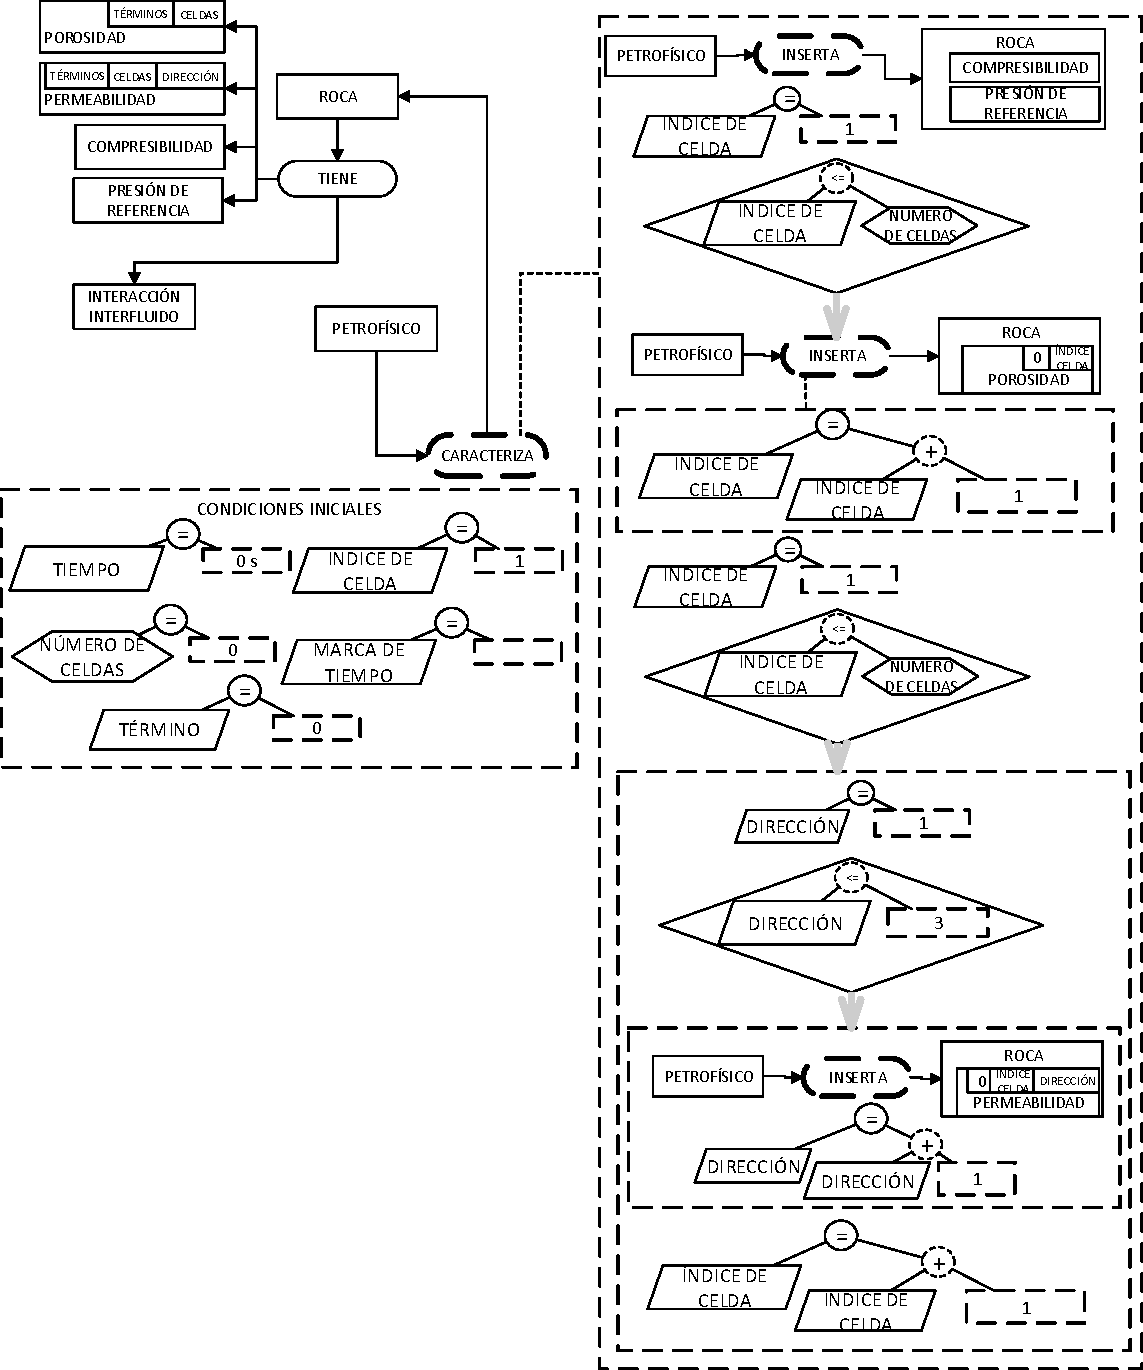
\includegraphics[width=1.5in]{Fig/Rock.pdf}\\ Ver figura \ref{fig:Rock}.\end{tabular}
			%
			%\caption[Elementos para la representación de Software Científico.]{Elementos para la representación de Software Científico. \citep{JCalle,norena2018det}.} \label{fig:RockTranslation}
		}
		&
		\begin{tiny}
			\begin{lstlisting}
			void Rock::characterize(const int& cells_number){
			
			std::ostringstream ss = std::ostringstream();
			const std::string axisnames[3]={"x", "y", "z"};
			
			_absolute_permeability = std::vector<std::vector<std::vector<double>>>
			(1,std::vector<std::vector<double>>(cells_number,std::vector<double>(3)));
			_porosity              = std::vector<std::vector<double>>(1,std::vector<double>(cells_number));
			
			myRead(std::string("Please insert rock compressibility [1/Pa]"), _compressibility,
			std::string("Please insert a valid input"));
			
			myRead(std::string("Please insert reference pressure [Pa]"), _reference_pressure,
			std::string("Please insert a valid input"));
			
			for(int cellindex=0; cellindex<cells_number; ++cellindex){
			
			ss << "Please insert initial porosity for the "<< cellindex+1 << " cell [-]";
			myRead(ss.str(), _porosity[0][cellindex], std::string("Please insert a valid input"));
			ss.str("");
			ss.clear();
			
			
			};
			for(int cellindex=0; cellindex<cells_number; ++cellindex){
			for(int direction=0; direction<3;++direction){
			ss << "Please insert initial absolute permeability for the "<< cellindex+1
			<< " cell in direction " << axisnames[direction] << " [m2]";
			myRead(ss.str(), _absolute_permeability[0][cellindex][direction],
			std::string("Please insert a valid input"));
			ss.str("");
			ss.clear();
			};
			};
			};
			
			\end{lstlisting}
		\end{tiny}
	\end{tabular}
	\caption[Traducción a código de la relación dinámica ``Petrofísico caracteriza Roca''.]{Traducción a código de la relación dinámica ``Petrofísico caracteriza Roca''. Los autores. \label{tab:RockCharacterizeCode}}
\end{table}
\newpage

En el código de la Tabla \ref{tab:ResidualCode} se evidencia cómo se logra iterar entre los conceptos. Por ejemplo para las ecuaciones, usando los vectores con los que se emula la base de datos, se logra realizar el cálculo del residual consistentemente con la representación. La operación de obtención de tipo, se desarrolla como un método interno dentro de la clase \textit{Equation\_Base}, con el fin de mantener la equivalencia casi exacta entre la representación y el código C++. Luego, la operación de asignación de tipo de ecuación, a fluido o a pozo, se convierte en una conversión de tipo o \textit{cast}.

\begin{table}[h!]
	\centering
	\begin{tabular}{cc}
		\parbox[c]{7em}{
			\begin{tabular}[c]{@{}c@{}}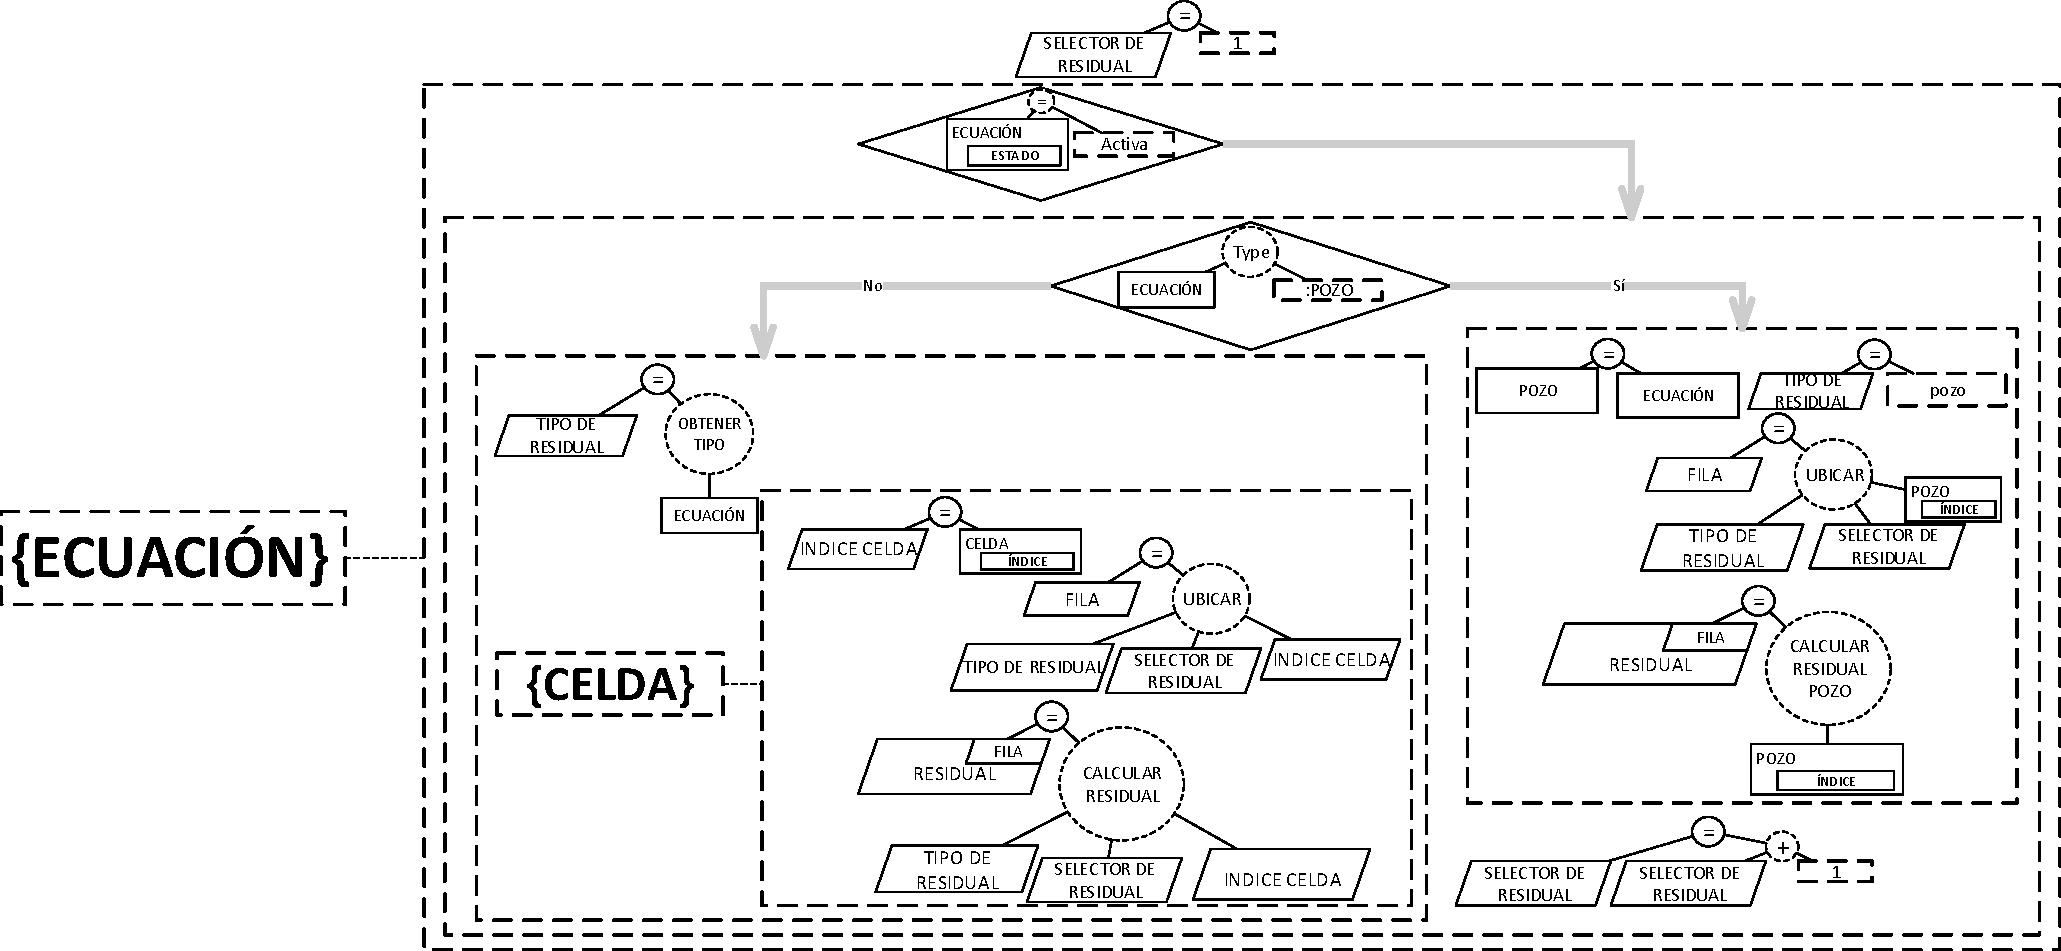
\includegraphics[width=2.5in]{Fig/Residual.pdf}\\ Ver figura \ref{fig:Residual}.\end{tabular}
			%
			%\caption[Elementos para la representación de Software Científico.]{Elementos para la representación de Software Científico. \citep{JCalle,norena2018det}.} \label{fig:RockTranslation}
		}
		&
		\begin{tiny}
			\begin{lstlisting}
			//Residual calculation
			residual_selector = 0;
			
			for(auto equation : equations){
			
			if(equation->status()){
			
			if(equation->type() == typeid(Well).name()){
			
			constexpr auto residual_type = "well";
			auto residual_well = std::dynamic_pointer_cast<Well,Equation_Base>(equation);
			
			row = locate(residual_type, residual_selector, residual_well->index());
			_residual(row) = calculateWellResidual(term, residual_well);
			
			}else{
			
			constexpr auto residual_type = "fluid";
			auto residual_fluid = std::dynamic_pointer_cast<Fluid,Equation_Base>(equation);
			
			for(auto cell = mesh.begin(); cell != mesh.end(); ++cell){
			
			cell_index = (*cell)->index();
			
			row = locate(residual_type, residual_selector, cell_index);
			
			_residual(row) = 
			calculateResidual(term,*residual_fluid, mesh, *cell, rock, wells);
			
			};
			};
			
			++residual_selector;
			
			};
			};
			
			\end{lstlisting}
		\end{tiny}
	\end{tabular}
	\caption[Traducción a código del cálculo de residual en el evento ``Presión del Fluido Varía''.]{Traducción a código del cálculo de residual en el evento ``Presión del Fluido Varía''. Los autores. \label{tab:ResidualCode}}
\end{table}


\section{Caso de Literatura}
En esta Sección se pretende validar el modelo ejecutable que se realiza a partir del esquema preconceptual. Con éste propósito, se plantea un caso que se toma de \cite{jamal2006petroleum}. El cual, consiste en una simulación de un yacimiento lineal (1D) de cinco celdas con un solo fluido y un pozo productor en la cuarta celda, como se muestra en la Figura \ref{fig:Abou-Kassem} \citep{jamal2006petroleum}. Con este, se espera validar el transporte de un fluido y las pérdidas de presión por pozos.\\

\begin{figure}[h]
	\centering
	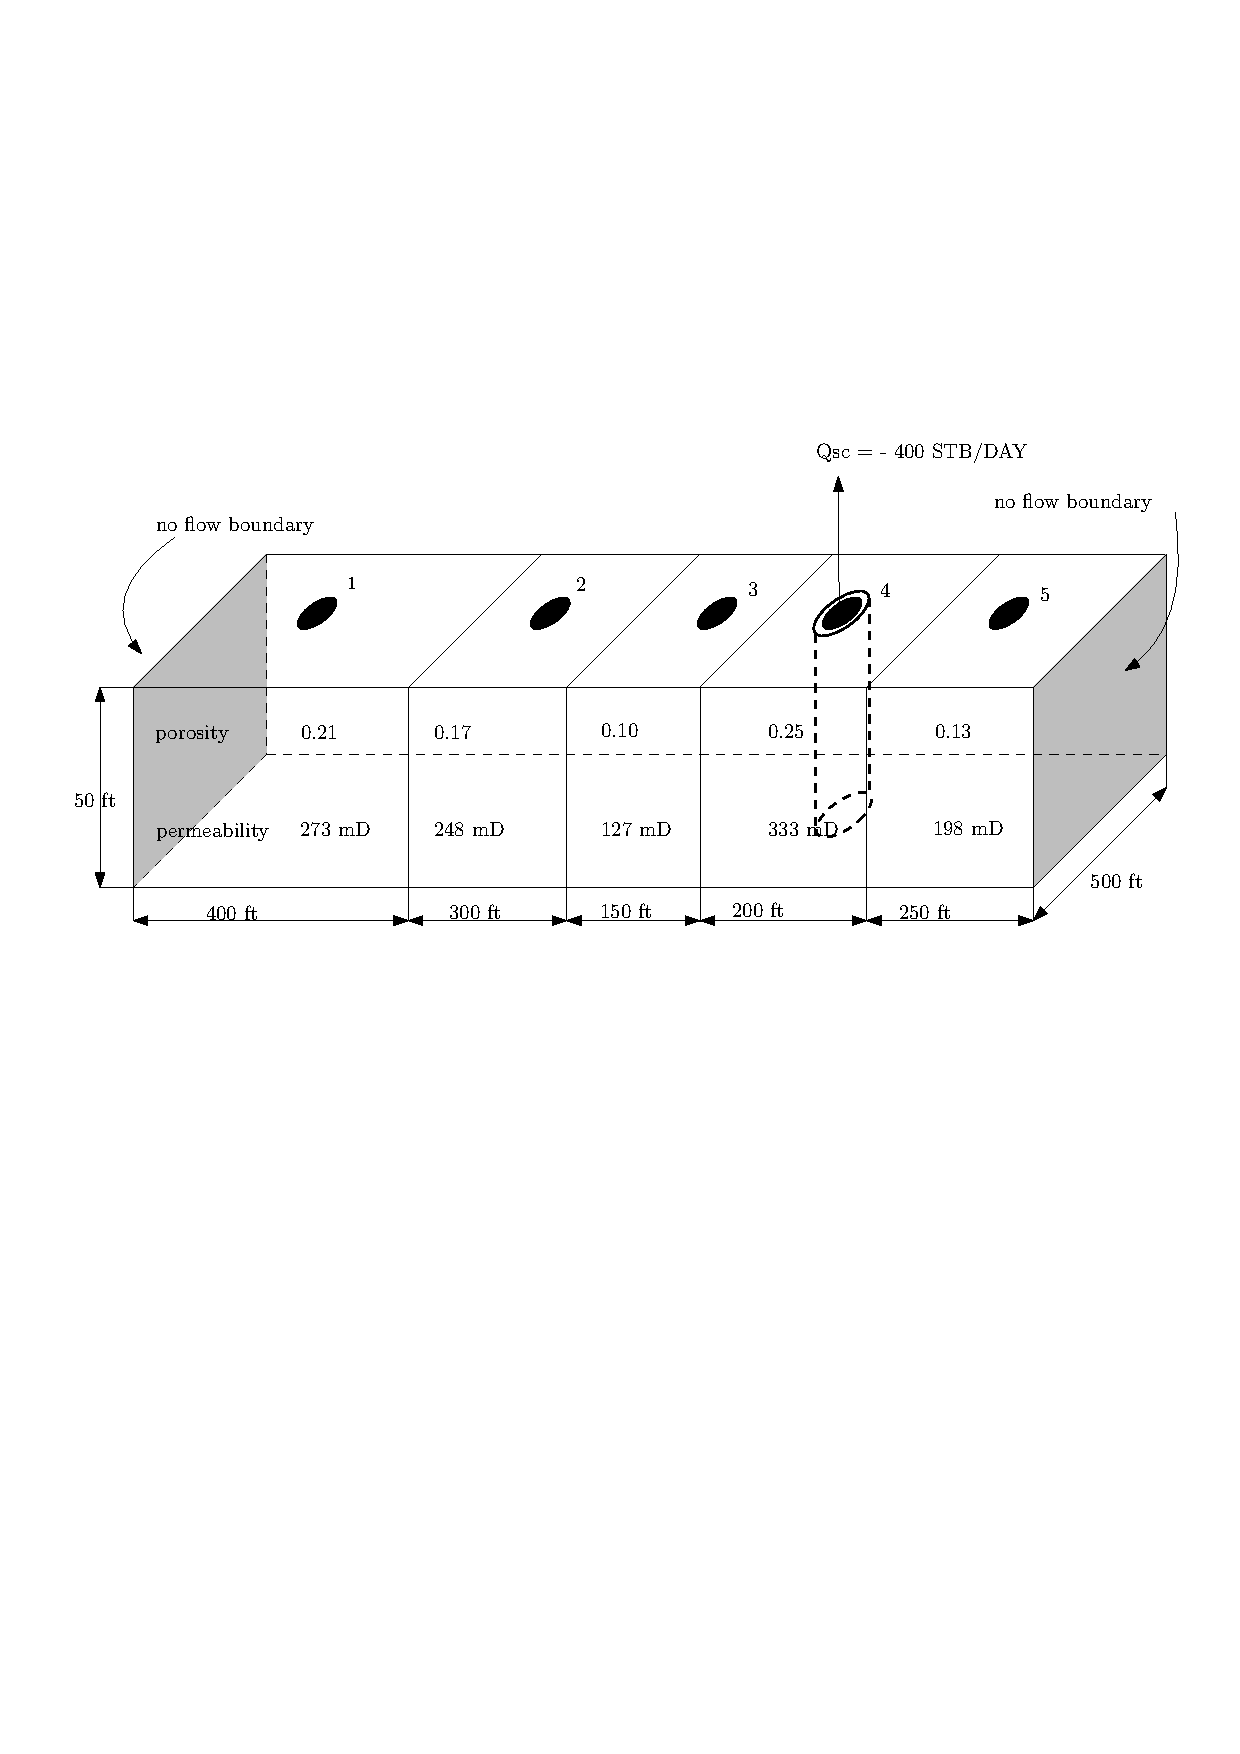
\includegraphics[width=0.9\textwidth]{Fig/casoasis.pdf}
	\caption{Representación gráfica del caso proporcionado por \cite{jamal2006petroleum}.}
	\label{fig:Abou-Kassem}
\end{figure}

El caso de estudio de \cite{jamal2006petroleum} consta de dos procesos principales, uno de pérdidas a caudal fijo, y el otro, cuando la celda perforada para el pozo alcanza la ``presión de abandono''. En este, se cambia la condición operativa del pozo para mantener la presión fija a esa presión de abandono. En la Figura \ref{fig:ConstantQ} se reportan los resultados de la simulación durante la etapa de producción a caudal constante, y en la Figura \ref{fig:ConstantP} se reportan los resultados de la simulación durante la etapa de producción a presión constante.\\





\begin{figure}[h]
	\centering
\begin{tikzpicture}
\begin{axis}[
title={Perdidas de presión a caudal fijo. Simulado vs Reportado},
xlabel={Celda},
ylabel={Presión (psi)},
xmin=0, xmax=6,
ymin=1500, ymax=3000,
legend pos=outer north east ,
ymajorgrids=true,
xmajorgrids=true,
%semilogxaxis=true,
grid style=dashed,
]

\addplot[color=blue]
coordinates{
	(1,2933.8141602)
	(2,2923.5889812)
	(3,2908.882128)
	(4,2896.698936)
	(5,2899.4836656)
	
};
\addlegendentry{5 días, simulado.}

\addplot[dashed, color=red]
coordinates{
	(1,2605.9267536)
	(2,2595.745086)
	(3,2581.1107518)
	(4,2569.0000788)
	(5,2571.741297)
	
};
\addlegendentry{25 días, simulado.}

\addplot[dotted,color=black]
coordinates{
	(1,2203.1127162)
	(2,2193.0180714)
	(3,2178.5287752)
	(4,2166.5196288)
	(5,2169.2463432)
	
};
\addlegendentry{50 días, simulado.}

\addplot[dashdotted,color=purple]
coordinates{
	(1,1729.7812032)
	(2,1719.8025888)
	(3,1705.4728344)
	(4,1693.6087260)
	(5,1696.3064328)
};
\addlegendentry{80 días, simulado.}

\addplot[only marks, mark options={draw=blue,fill=blue,}]
coordinates{
	(1,2936.80)
	(2,2928.38)
	(3,2915.68)
	(4,2904.88)
	(5,2908.18)
	
	
};
\addlegendentry{5 días, reportado.}
\addplot[only marks, mark=square*, mark options={draw=red,fill=red,}]
coordinates{
	(1,2630.34)
	(2,2620.06)
	(3,2605.28)
	(4,2593.04)
	(5,2595.81)
	
	
};
\addlegendentry{25 días, reportado.}
\addplot[only marks, mark=diamond*, mark options={draw=black,fill=black,}]
coordinates{
	(1,2243.97)
	(2,2233.68)
	(3,2218.9)
	(4,2206.66)
	(5,2209.43)
	
	
};
\addlegendentry{50 días, reportado.}
\addplot[only marks, mark=triangle*, mark options={draw=purple,fill=purple,}]
coordinates{
	
	(1,1780.3100)
	(2,1770.0200)
	(3,1755.2400)
	(4,1743.0000)
	(5,1745.7700)
	
	
};
\addlegendentry{80 días, reportado.}
\end{axis}
\end{tikzpicture}
\caption{Comparativo datos simulados contra caso de estudio de \cite{jamal2006petroleum}. Caudal constante.}
\label{fig:ConstantQ}
\end{figure}{}

Las condiciones iniciales de presión para el yacimiento son de $3000$ $psia$ para todas las celdas y el pozo se establece a una condición operativa de caudal fijo a $400$ $STB/D$. Se puede ver como en los primeros 80 días, va decayendo la presión hasta alcanzar la presión de abandono. Se encuentran diferencias entre los resultados simulados y los reportados por \cite{jamal2006petroleum} menores a $50$ $psia$. Éstas se deben, a que las ecuaciones que se implementan en el modelo ejecutable, son diferentes a las que se presentan en \cite{jamal2006petroleum}.\\

\begin{figure}[h]
	\centering
	\begin{tikzpicture}
	\begin{axis}[
	title={Pérdidas de presión a presión fija. Simulado vs Reportado},
	xlabel={Celda},
	ylabel={Presión (psi)},
	xmin=0, xmax=6,
	ymin=1500, ymax=1550,
	legend pos=outer north east ,
	ymajorgrids=true,
	xmajorgrids=true,
	%semilogxaxis=true,
	grid style=dashed,
	]
	
	\addplot[color=blue]
	coordinates{
		(1,	1526.960064 )
		(2,	1522.7829696)
		(3,	1517.169999)
		(4,	1512.6593172)
		(5,	1513.1959578)
	};
	\addlegendentry{100 días, simulado.}
	
	\addplot[color=green]
	coordinates{
		(1,	1509.9326028)
		(2,	1508.4097038)
		(3,	1506.3356604)
		(4,	1504.6822272)
		(5,	1504.8852804)
	};
	\addlegendentry{105 días, simulado.}
	
	\addplot[color=black]
	coordinates{
		(1,	1503.6524574)
		(2,	1503.101313)
		(3,	1502.3326116)
		(4,	1501.723452)
		(5,	1501.795971)
	};
	\addlegendentry{110 días, simulado.}
	
	\addplot[color=purple]
	coordinates{
		(1,	1501.3463532)
		(2,	1501.1433)
		(3,	1500.853224)
		(4,	1500.635667)
		(5,	1500.6501708)
	};
	\addlegendentry{115 días, simulado.}
	
	\addplot[color=pink]
	coordinates{
		(1,	1500.490629)
		(2,	1500.41811)
		(3,	1500.3165834)
		(4,	1500.2295606)
		(5,	1500.2295606)
	};
	\addlegendentry{120 días, simulado.}
	
	
	\addplot[]
	coordinates{
		(1,	1500.1715454)
		(2,	1500.1425378)
		(3,	1500.1135302)
		(4,	1500.0845226)
		(5,	1500.0845226)
	};
	\addlegendentry{125 días, simulado.}
	
	\addplot[color=orange]
	coordinates{
		(1,	1500.055515)
		(2,	1500.0410112)
		(3,	1500.0265074)
		(4,	1500.0265074)
		(5,	1500.0265074)
	};
	\addlegendentry{130 días, simulado.}
	
	
	\addplot[red]
	coordinates{
		(1,	1500.0120036)
		(2,	1500.0120036)
		(3,	1500.0120036)
		(4,	1499.9974998)
		(5,	1499.9974998)
	};
	\addlegendentry{135 días, simulado.}
	
	
	\addplot[only marks]
	coordinates{
		(1,	1524.61)
		(2,	1520)
		(3,	1514)
		(4,	1509 )
		(5,	1510)
		
	};
	\addlegendentry{100 días, reportado. }
	
	\addplot[only marks]
	coordinates{
		(1,	1510.35)
		(2,	1508.46)
		(3,	1505.91)
		(4,	1503.88)
		(5,	1504.09)
		
	};
	\addlegendentry{105 días, reportado.}
	
	\addplot[only marks]
	coordinates{
		(1,	1504.34)
		(2,	1503.54)
		(3,	1502.47)
		(4,	1501.61)
		(5,	1501.7)
	};
	\addlegendentry{110 días, reportado. }
	
	\addplot[only marks]
	coordinates{
		(1,	1501.82)
		(2,	1501.48)
		(3,	1501.03)
		(4,	1500.68)
		(5,	1500.71)
	};
	\addlegendentry{115 días, reportado.}
	
	\addplot[only marks]
	coordinates{
		(1,	1500.76)
		(2,	1500.62)
		(3,	1500.43)
		(4,	1500.28)
		(5,	1500.3)
	};
	\addlegendentry{120 días, reportado.}
	
	
	\addplot[only marks]
	coordinates{
		(1,	1500.32)
		(2,	1500.26)
		(3,	1500.18)
		(4,	1500.12)
		(5,	1500.12)
	};
	\addlegendentry{125 días, reportado.}
	
	\addplot[only marks]
	coordinates{
		(1,	1500.13)
		(2,	1500.11)
		(3,	1500.08)
		(4,	1500.05)
		(5,	1500.05)
	};
	\addlegendentry{130 días, reportado.}
	
	
	\addplot[only marks]
	coordinates{
		(1	,1500.06)
		(2	,1500.05)
		(3	,1500.03)
		(4	,1500.02)
		(5	,1500.02)
	};
	\addlegendentry{135 días, reportado.}
	
	\end{axis}
	\end{tikzpicture}
	\caption{Comparativo datos simulados contra caso de estudio de \cite{jamal2006petroleum}. Presión constante.}
	\label{fig:ConstantP}
\end{figure}{}

En la etapa de producción a presión constante se logra observar como la presión del sistema decae hasta que se estabiliza completamente a la presión de abandono. En esta etapa se siguen observando diferencias de alrededor de $10$ $psia$. Con este comportamiento se logra validar el modelo ejecutable para la simulación de casos de producción por flujo natural. Para ejecutar casos en los que se involucren más fenómenos físicos, se requiere un control numérico adicional que no se contempla en el desarrollo de esta Tesis de Maestría.

\chapter{Conclusiones y trabajo futuro}\label{cap:Conclusiones}
\section{Conclusiones}


En esta Tesis de Maestría se establecieron los fenómenos de flujo o transporte, transferencia y de superficie en los procesos de recobro mejorado (EOR) para yacimientos de petróleo. A partir de tales fenómenos, se conceptualizaron los elementos del sistema, o dominio, y las interacciones físicas, y, químicas entre fluidos y agentes externos que se presentan en los procesos EOR. La estrategia de solución que se diseñó, permite acoplar diferentes mecanismos físicos y químicos de manera general, solucionando las ecuaciones algebraicas y diferenciales en las que se describen estos mecanismos. Con esta estrategia de solución, se construyó una simulación basada en un esquema preconceptual que hace las veces de modelo ejecutable y, que se logró validar con un caso de estudio en la literatura.\\

Si bien existen múltiples representaciones para la simulación de procesos de recobro mejorado, y se han realizado diferentes simulaciones a partir de sus modelos matemáticos, se logró evidenciar que muchas de estas carecen de trazabilidad entre conceptos y procesos que se ejecutan la simulación, induciendo a una falta de formalidad en el desarrollo de simuladores para procesos EOR. Este modelo ejecutable puede constituir una base para desarrollar simulaciones de procesos EOR, debido a que conserva la trazabilidad de los conceptos presentes y muestra el paso a paso de la ejecución de los procesos. Éste, también presenta elementos de generalización que permiten abarcar otros fenómenos. Además, la concordancia de los resultados con el caso de la literatura indica que el modelo ejecutable desarrollado tiene validez. Más aún, es posible, por medio de los eventos del EP, representar la aplicación de otros campos en el dominio físico, como, por ejemplo, los de temperatura y esfuerzos.\\

El desarrollo del esquema preconceptual ejecutable y su respectiva traducción a C++ es una clara muestra de la consistencia que se obtiene al trazar los conceptos y los procesos en el código y, la representación en el EP es acorde con la física y la conceptualización de los modelos matemáticos que se establecen para una simulación. Un elemento importante en el modelo ejecutable es la capacidad de encapsular e iterar sobre conceptos, generando independencia entre los mismos. Esto provee la flexibilidad suficiente para generalizar los modelos que se utilizan en la simulación de yacimientos de petróleo, y cambiar especificaciones sin modificar el modelo ejecutable.

\section{Trabajo futuro}

A partir de esta Tesis de Maestría se identifican varias líneas de investigación por desarrollar:

\begin{itemize}
	\item Representar la fenomenología de diferentes químicos usando el modelo ejecutable definido.
	\item Modelar un simulador composicional de flujo basado en esquemas preconceptuales.
	\item Explorar diferentes esquemas de solución numérica para la simulación de procesos de recobro mejorado en yacimientos de petróleo.
	\item Identificar patrones de diseño en el modelo ejecutable basado en esquemas preconceptuales definido.
\end{itemize}

%Se presentan como una serie de aspectos que se podr\'{\i}an realizar en un futuro para emprender investigaciones similares o fortalecer la investigaci\'{o}n realizada. Deben contemplar las perspectivas de la investigaci\'{o}n, las cuales son sugerencias, proyecciones o alternativas que se presentan para modificar, cambiar o incidir sobre una situaci\'{o}n espec\'{\i}fica o una problem\'{a}tica encontrada. Pueden presentarse como un texto con caracter\'{\i}sticas argumentativas, resultado de una reflexi\'{o}n acerca de la tesis o trabajo de investigaci\'{o}n.\\
\begin{appendix}
\chapter{Anexo: Discretización de las Ecuaciones del BOM}\label{AnexoA}
En este apartado se presenta la discretización de las Ecuaciones del BOM \ref{ec:aceite}, \ref{ec:gas}, \ref{ec:agua} que se presentan en la subsección \ref{subsec:BOM}. Recordando:
\begin{align*}
\text{aceite: }&\frac{\partial}{\partial t} \left[ \phi \left( \frac{S_{o}}{B_{o}} + \frac{R_{v} S_{g}}{B_{g}} \right) \right]
- \nabla \cdot \left( \frac{1}{B_{o}} \vec{u_{o}} + \frac{R_{v}}{B_{g}} \vec{u_{g}} \right) - \tilde{q}_{o}=0  \\
\text{gas: }&\frac{\partial}{\partial t} \left[ \phi \left( \frac{S_{g}}{B_{g}} + \frac{R_{s} S_{o}}{B_{o}} \right) \right]
- \nabla \cdot \left( \frac{1}{B_{g}} \vec{u_{g}} + \frac{R_{s}}{B_{o}} \vec{u_{o}} \right) - \tilde{q}_{g} = 0 \\
\text{agua: }&\frac{\partial}{\partial t} \left[\phi \left( \frac{S_{w}}{B_{w}} \right) \right] - \nabla \cdot \left( \frac{1}{B_{w}} \vec{u_{w}} \right) - \tilde{q}_{w} = 0 
\end{align*}
Primero, se integran las ecuaciones sobre un intervalo de tiempo $\left[t, t+\Delta t\right]$, y una celda de control $\Omega_{i}$. Se toma como ejemplo la ecuación de conservación para el aceite \ref{ec:aceite}. Las ecuaciones para el gas y agua (\ref{ec:gas}, \ref{ec:agua}) se discretizan de manera análoga.
\begin{align*}
	\int_{t}^{t+\Delta t}\int_{\Omega_{i}}\frac{\partial}{\partial t} \left[ \phi \left( \frac{S_{o}}{B_{o}} + \frac{R_{v} S_{g}}{B_{g}} \right) \right]dVdt
	- \int_{t}^{t+\Delta t}\int_{\Omega_{i}}\nabla \cdot \left( \frac{1}{B_{o}} \vec{u_{o}} + \frac{R_{v}}{B_{g}} \vec{u_{g}} \right)dVdt \\
	- \int_{t}^{t+\Delta t}\int_{\Omega_{i}}\tilde{q}_{o}dVdt=0 
\end{align*}
Luego, se desglosan las ecuaciones en sus términos acumulativos, de flujo, y de fuentes y sumideros, debido a que cada uno de estos términos requiere un tratamiento distinto.
\begin{align*}
\underbrace{\int_{t}^{t+\Delta t}\int_{\Omega_{i}}\frac{\partial}{\partial t} \left[ \phi \left( \frac{S_{o}}{B_{o}} + \frac{R_{v} S_{g}}{B_{g}} \right) \right]dVdt}_{\text{Término de acumulación}}
- \underbrace{\int_{t}^{t+\Delta t}\int_{\Omega_{i}}\nabla \cdot \left( \frac{1}{B_{o}} \vec{u_{o}} + \frac{R_{v}}{B_{g}} \vec{u_{g}} \right)dVdt}_\text{Término de flujo} \\
- \underbrace{\int_{t}^{t+\Delta t}\int_{\Omega_{i}}\tilde{q}_{o}dVdt}_{\text{Término de fuentes y sumideros}}=0 
\end{align*}
Empezando por el término acumulativo, se sigue que, por el teorema de Fubini que
\begin{align*}
	\int_{t}^{t+\Delta t}\left(\int_{\Omega_{i}}\frac{\partial}{\partial t} \left[ \phi \left( \frac{S_{o}}{B_{o}} + \frac{R_{v} S_{g}}{B_{g}} \right) \right]dV\right)dt = \int_{\Omega_{i}}\left(\int_{t}^{t+\Delta t}\frac{\partial}{\partial t} \left[ \phi \left( \frac{S_{o}}{B_{o}} + \frac{R_{v} S_{g}}{B_{g}} \right) \right]dt\right)dV 
\end{align*}
Por teorema fundamental del cálculo
\begin{align*}
 \int_{\Omega_{i}}\left(\int_{t}^{t+\Delta t}\frac{\partial}{\partial t} \left[ \phi \left( \frac{S_{o}}{B_{o}} + \frac{R_{v} S_{g}}{B_{g}} \right) \right]dt\right)dV = \int_{\Omega_{i}}\left[ \phi \left( \frac{S_{o}}{B_{o}} + \frac{R_{v} S_{g}}{B_{g}} \right) \right]^{t+\Delta t}_{t}dV
\end{align*}
Considerando el cambio de la acumulación en un intervalo de tiempo como una constante para una celda de control $\Omega_{i}$
\begin{align*}
	\int_{\Omega_{i}}\left[ \phi \left( \frac{S_{o}}{B_{o}} + \frac{R_{v} S_{g}}{B_{g}} \right) \right]^{t+\Delta t}_{t}dV = \left[ \phi_{i} \left( \frac{S_{o,i}}{B_{o,i}} + \frac{R_{v,i} S_{g,i}}{B_{g,i}} \right) \right]^{t+\Delta t}_{t}\int_{\Omega_{i}}dV \\= |\Omega_{i}|\left[ \phi_{i} \left( \frac{S_{o,i}}{B_{o,i}} + \frac{R_{v,i} S_{g,i}}{B_{g,i}} \right) \right]^{t+\Delta t}_{t}
\end{align*}
Donde $|\Omega_{i}|$ es el volumen para una celda $i$. Continuando con la discretización del término de flujo, se discretiza primero el tiempo usando un esquema \textbf{implícito}, luego
\begin{align*}
\int_{t}^{t+\Delta t}\int_{\Omega_{i}}\nabla \cdot \left( \frac{1}{B_{o}} \vec{u_{o}} + \frac{R_{v}}{B_{g}} \vec{u_{g}} \right)dVdt = \Delta t \left[\int_{\Omega_{i}}\nabla \cdot \left( \frac{1}{B_{o}} \vec{u_{o}} + \frac{R_{v}}{B_{g}} \vec{u_{g}} \right)dV\right]^{t+\Delta t}
\end{align*}
Posteriormente, se asume que la función vectorial de velocidad $\vec{u_{f}}$ para cualquier fluido $f$ tiene derivadas de primer orden continuas. Luego, como la celda tiene una superficie cerrada, se aplica el teorema de la divergencia Gauss.
\begin{align*}
	\int_{\Omega_{i}}\nabla \cdot \left( \frac{1}{B_{o}} \vec{u_{o}} + \frac{R_{v}}{B_{g}} \vec{u_{g}} \right)dV = \int_{\partial \Omega_{i}}\left( \frac{1}{B_{o}} \vec{u_{o}} + \frac{R_{v}}{B_{g}} \vec{u_{g}} \right)\cdot \partial \vec{S_{i}}
\end{align*}
Usando celdas rectangulares, la integral sobre la frontera de una celda es la suma del término de flujo que se evalúa en cada cara, así
\begin{align*}
 \int_{\partial \Omega_{i}}\left( \frac{1}{B_{o}} \vec{u_{o}} + \frac{R_{v}}{B_{g}} \vec{u_{g}} \right)\cdot \partial \vec{S_{i}} = \sum_{c \in S_{i}}\int_{c}\left( \frac{1}{B_{o}} \vec{u_{o}} + \frac{R_{v}}{B_{g}} \vec{u}_{g} \right)\cdot \partial \vec{S_{c}}
\end{align*}
El valor del término de flujo en cada cara se aproxima usando el teorema del valor medio, luego el producto punto se evalua como el valor de la función en la cara
\begin{align*}
	\sum_{c \in S_{i}}\int_{c}\left( \frac{1}{B_{o}} \vec{u_{o}} + \frac{R_{v}}{B_{g}} \vec{u_{g}} \right)\cdot \partial \vec{S_{c}} \approx \sum_{c \in S_{i}} A_{c} \left( \frac{1}{B_{o,c}} \vec{u_{o,c}} + \frac{R_{v,c}}{B_{g,c}} \vec{u_{g,c}} \right)
\end{align*}
Aplicando las velocidades Darcy en la ecuación, se tiene
\begin{align*}
	\sum_{c \in S_{i}} A_{c} \left( \frac{1}{B_{o,c}} \vec{u_{o,c}} + \frac{R_{v,c}}{B_{g,c}} \vec{u_{g,c}} \right) \cdot \vec{n_{c}} = \sum_{c \in S_{i}} A_{c} \left( \frac{1}{B_{o,c}} \frac{\mathbb{K}_{c}k_{ro,c}}{\mu_{o,c}} \nabla \Phi_{o,c} + \frac{R_{v,c}}{B_{g,c}} \frac{\mathbb{K}_{c}k_{rg,c}}{\mu_{g,c}} \nabla \Phi_{g,c} \right)
\end{align*}
Dónde el gradiente de potencial $\nabla \Phi_{f,c}$, para cualquier fluido $f$ se aproxima como:
\begin{align*}
	\nabla \Phi_{f,c} \approx \frac{\Delta \Phi_{f,c}}{\Delta l_{c}} \approx \frac{\Phi_{f,i}-\Phi_{f,j}}{\Delta l_{c}}
\end{align*}
Donde $c$ es la cara que conecta la celda $i$ con la celda $j$, y el delta de longitud en la cara $\Delta l_{c}$ se calcula como:
\begin{align}
	\label{ec:DeltaCara}\Delta l_{c} = \frac{\Delta l_{i} + \Delta l_{j}}{2}
\end{align}
Cabe notar que, los deltas de longitud dependen de la dirección del vector normal $\vec{n}$. Por último, el término de fuentes y sumideros se aproxima de la misma manera que el termino del flujo, usando el teorema de valor medio. Así
\begin{align*}
	\int_{t}^{t+\Delta t}\int_{\Omega_{i}}\tilde{q}_{o}dVdt \approx \int_{t}^{t+\Delta t}\tilde{q}_{o,i} |\Omega_{i}|dt
	\approx \left[\tilde{q}_{o,i}\right]^{t+\Delta t} |\Omega_{i}|\Delta t
\end{align*}
tomando los tiempos $t+\Delta t$ como tiempo futuro o $n+1$ y los tiempo $t$ como tiempo pasado $n$, se obtiene la discretización de la ecuación de conservación del aceite (\ref{ec:aceiteDiscretizacion}) como:
\begin{align*}
	|\Omega_{i}|\left[ \phi_{i} \left( \frac{S_{o,i}}{B_{o,i}} + \frac{R_{v,i} S_{g,i}}{B_{g,i}} \right) \right]^{n+1}_{n} - \Delta t \sum_{c \in S_{i}} A_{c} \left[ \frac{1}{B_{o,c}} \frac{\mathbb{K}_{c}k_{ro,c}}{\mu_{o,c}} \nabla \Phi_{o,c} + \frac{R_{v,c}}{B_{g,c}} \frac{\mathbb{K}_{c}k_{rg,c}}{\mu_{g,c}} \nabla \Phi_{g,c} \right]^{n+1} \\- \left[\tilde{q}_{o,i}\right]^{n+1} |\Omega_{i}|\Delta t = 0
\end{align*}
Se define el término de transmisividad, en el cual se considera un promedio armónico que se utiliza para estimar el término $\mathbb{K}_{c}$ y se involucra la Ecuación \ref{ec:DeltaCara}, de la siguiente forma:
\begin{align*}
	&T_{o,c} = \left(\frac{2}{(\Delta l_{i}/A_{c}K_{l,i})+(\Delta l_{j}/A_{c}K_{l,j})}\right)\frac{k_{ro,c}}{\mu_{o,c}B_{o,c}}\\
	&T_{g,c} = \left(\frac{2}{(\Delta l_{i}/A_{c}K_{l,i})+(\Delta l_{j}/A_{c}K_{l,j})}\right)\frac{k_{rg,c}}{\mu_{g,c}B_{g,c}}
\end{align*}
Luego la ecuación de conservación que se discretiza queda:
\begin{align*}
|\Omega_{i}|\left[ \phi_{i} \left( \frac{S_{o,i}}{B_{o,i}} + \frac{R_{v,i} S_{g,i}}{B_{g,i}} \right) \right]^{n+1}_{n} - \Delta t \sum_{c \in S_{i}} \left[ T_{o,c} \Delta \Phi_{o,c} + R_{v,c} T_{g,c} \nabla \Phi_{g,c} \right]^{n+1} - \left[\tilde{q}_{o,i}\right]^{n+1} |\Omega_{i}|\Delta t = 0
\end{align*}

Considerando $\left[\tilde{q}_{o,i}\right]^{n+1} |\Omega_{i}|$ como un flujo volumétrico $\left[Q_{o,i}\right]^{n+1}$ e involucrando la evaluación al tiempo $n+1$ en cada uno de los términos, se tiene:
\begin{align*}
|\Omega_{i}|\left[ \phi_{i} \left( \frac{S_{o,i}}{B_{o,i}} + \frac{R_{v,i} S_{g,i}}{B_{g,i}} \right) \right]^{n+1}_{n} - \Delta t \sum_{c \in S_{i}} \left[ T_{o,c}^{n+1} \Delta \Phi_{o,c}^{n+1} + R_{v,c}^{n+1} T_{g,c}^{n+1} \Delta \Phi_{g,c}^{n+1} \right] - Q_{o,i}^{n+1} \Delta t
\end{align*}
Finalmente, dividiendo por $\Delta t$ la ecuación se obtiene:
\begin{align*}
\frac{|\Omega_{i}|}{\Delta t}\left[ \phi_{i} \left( \frac{S_{o,i}}{B_{o,i}} + \frac{R_{v,i} S_{g,i}}{B_{g,i}} \right) \right]^{n+1}_{n} - \sum_{c \in S_{i}} \left[ T_{o,c}^{n+1} \Delta \Phi_{o,c}^{n+1} + R_{v,c}^{n+1} T_{g,c}^{n+1} \Delta \Phi_{g,c}^{n+1} \right] - Q_{o,i}^{n+1} = 0
\end{align*}
La discretización de las ecuaciones de conservación para el gas y el agua (\ref{ec:gas}, \ref{ec:agua}) se obtienen de manera análoga a la del aceite.
\chapter{Anexo: Traducciones a código de la representación}
A final del documento es opcional incluir \'{\i}ndices o glosarios. \'{E}stos son listas detalladas y especializadas de los t\'{e}rminos, nombres, autores, temas, etc., que aparecen en el mismo. Sirven para facilitar su localizaci\'{o}n en el texto. Los \'{\i}ndices pueden ser alfab\'{e}ticos, cronol\'{o}gicos, num\'{e}ricos, anal\'{\i}ticos, entre otros. Luego de cada palabra, t\'{e}rmino, etc., se pone coma y el n\'{u}mero de la p\'{a}gina donde aparece esta informaci\'{o}n.\\

\chapter{Anexo: Nombrar el anexo C de acuerdo con su contenido}
MANEJO DE LA BIBLIOGRAF\'{I}A: la bibliograf\'{\i}a es la relaci\'{o}n de las fuentes documentales consultadas por el investigador para sustentar sus trabajos. Su inclusi\'{o}n es obligatoria en todo trabajo de investigaci\'{o}n. Cada referencia bibliogr\'{a}fica se inicia contra el margen izquierdo.\\

La NTC 5613 establece los requisitos para la presentaci\'{o}n de referencias bibliogr\'{a}ficas citas y notas de pie de p\'{a}gina. Sin embargo, se tiene la libertad de usar cualquier norma bibliogr\'{a}fica de acuerdo con lo acostumbrado por cada disciplina del conocimiento. En esta medida es necesario que la norma seleccionada se aplique con rigurosidad.\\

Es necesario tener en cuenta que la norma ISO 690:1987 (en Espa\~{n}a, UNE 50-104-94) es el marco internacional que da las pautas m\'{\i}nimas para las citas bibliogr\'{a}ficas de documentos impresos y publicados. A continuaci\'{o}n se lista algunas instituciones que brindan par\'{a}metros para el manejo de las referencias bibliogr\'{a}ficas:\\

\begin{center}
\centering%
\begin{tabular}{|p {7.5 cm}|p {7.5 cm}|}\hline
\arr{Instituci\'{o}n}&Disciplina de aplicaci\'{o}n\\\hline%
Modern Language Association (MLA)&Literatura, artes y humanidades\\\hline%
American Psychological Association (APA)&Ambito de la salud (psicolog\'{\i}a, medicina) y en general en todas las ciencias sociales\\\hline
Universidad de Chicago/Turabian &Periodismo, historia y humanidades.\\\hline
AMA (Asociaci\'{o}n M\'{e}dica de los Estados Unidos)&Ambito de la salud (psicolog\'{\i}a, medicina)\\\hline
Vancouver &Todas las disciplinas\\\hline
Council of Science Editors (CSE)&En la actualidad abarca diversas ciencias\\\hline
National Library of Medicine (NLM) (Biblioteca Nacional de Medicina)&En el \'{a}mbito m\'{e}dico y, por extensi\'{o}n, en ciencias.\\\hline
Harvard System of Referencing Guide &Todas las disciplinas\\\hline
JabRef y KBibTeX &Todas las disciplinas\\\hline
\end{tabular}
\end{center}

Para incluir las referencias dentro del texto y realizar lista de la bibliograf\'{\i}a en la respectiva secci\'{o}n, puede utilizar las herramientas que Latex suministra o, revisar el instructivo desarrollado por el Sistema de Bibliotecas de la Universidad Nacional de Colombia\footnote{Ver: www.sinab.unal.edu.co}, disponible en la secci\'{o}n "Servicios", opci\'{o}n "Tr\'{a}mites" y enlace "Entrega de tesis".

\chapter{Sizas Tikz}
{\color{red} \LARGE Ojo! Esto no es un anexo, es solo para pruebas}
\begin{figure}[h!]
	\begin{tikzpicture}
	\begin{axis}[
	title={Datos simulados por el Autor contra caso de estudio.},
	xlabel={Bloque},
	ylabel={Presión (psi)},
	xmin=0, xmax=6,
	ymin=1500, ymax=1550,
	legend pos=outer north east ,
	ymajorgrids=true,
	xmajorgrids=true,
	%semilogxaxis=true,
	grid style=dashed,
	]
	
	\addplot[color=blue]
	coordinates{
		(1,	1526.960064 )
		(2,	1522.7829696)
		(3,	1517.169999)
		(4,	1512.6593172)
		(5,	1513.1959578)
	};
	\addlegendentry{5 días. Autor.}
	
	\addplot[color=green]
	coordinates{
		(1,	1509.9326028)
		(2,	1508.4097038)
		(3,	1506.3356604)
		(4,	1504.6822272)
		(5,	1504.8852804)
	};
	\addlegendentry{10 días. Autor.}
	
	\addplot[color=black]
	coordinates{
		(1,	1503.6524574)
		(2,	1503.101313)
		(3,	1502.3326116)
		(4,	1501.723452)
		(5,	1501.795971)
	};
	\addlegendentry{15 días. Autor.}
	
	\addplot[color=purple]
	coordinates{
		(1,	1501.3463532)
		(2,	1501.1433)
		(3,	1500.853224)
		(4,	1500.635667)
		(5,	1500.6501708)
	};
	\addlegendentry{20 días. Autor.}
	
	\addplot[color=pink]
	coordinates{
		(1,	1500.490629)
		(2,	1500.41811)
		(3,	1500.3165834)
		(4,	1500.2295606)
		(5,	1500.2295606)
	};
	\addlegendentry{25 días. Autor.}
	
	
	\addplot[]
	coordinates{
		(1,	1500.1715454)
		(2,	1500.1425378)
		(3,	1500.1135302)
		(4,	1500.0845226)
		(5,	1500.0845226)
	};
	\addlegendentry{30 días. Autor.}
	
	\addplot[color=orange]
	coordinates{
		(1,	1500.055515)
		(2,	1500.0410112)
		(3,	1500.0265074)
		(4,	1500.0265074)
		(5,	1500.0265074)
	};
	\addlegendentry{35 días. Autor.}
	
	
	\addplot[red]
	coordinates{
		(1,	1500.0120036)
		(2,	1500.0120036)
		(3,	1500.0120036)
		(4,	1499.9974998)
		(5,	1499.9974998)
	};
	\addlegendentry{40 días. Autor.}
	
	
	\addplot[only marks]
	coordinates{
		(1,	1524.61)
		(2,	1520)
		(3,	1514)
		(4,	1509 )
		(5,	1510)
		
	};
	\addlegendentry{5 días. }
	
	\addplot[only marks]
	coordinates{
		(1,	1510.35)
		(2,	1508.46)
		(3,	1505.91)
		(4,	1503.88)
		(5,	1504.09)
		
	};
	\addlegendentry{10 días.}
	
	\addplot[only marks]
	coordinates{
		(1,	1504.34)
		(2,	1503.54)
		(3,	1502.47)
		(4,	1501.61)
		(5,	1501.7)
	};
	\addlegendentry{15 días. }
	
	\addplot[only marks]
	coordinates{
		(1,	1501.82)
		(2,	1501.48)
		(3,	1501.03)
		(4,	1500.68)
		(5,	1500.71)
	};
	\addlegendentry{20 días.}
	
	\addplot[only marks]
	coordinates{
		(1,	1500.76)
		(2,	1500.62)
		(3,	1500.43)
		(4,	1500.28)
		(5,	1500.3)
	};
	\addlegendentry{25 días.}
	
	
	\addplot[only marks]
	coordinates{
		(1,	1500.32)
		(2,	1500.26)
		(3,	1500.18)
		(4,	1500.12)
		(5,	1500.12)
	};
	\addlegendentry{30 días.}
	
	\addplot[only marks]
	coordinates{
		(1,	1500.13)
		(2,	1500.11)
		(3,	1500.08)
		(4,	1500.05)
		(5,	1500.05)
	};
	\addlegendentry{35 días.}
	
	
	\addplot[only marks]
	coordinates{
		(1	,1500.06)
		(2	,1500.05)
		(3	,1500.03)
		(4	,1500.02)
		(5	,1500.02)
	};
	\addlegendentry{40 días.}
	
	\end{axis}
	\end{tikzpicture}
	\caption{gg}
	\label{cora}
\end{figure}{}


\begin{figure}[h!]
	\begin{tikzpicture}
	\begin{axis}[
	title={Datos simulados por el Autor contra caso de estudio.},
	xlabel={Bloque},
	ylabel={Presión (psi)},
	xmin=0, xmax=6,
	ymin=1500, ymax=3000,
	legend pos=outer north east ,
	ymajorgrids=true,
	xmajorgrids=true,
	%semilogxaxis=true,
	grid style=dashed,
	]
	
	\addplot[]
	coordinates{
		(1,2933.8141602)	
		(2,2923.5889812)	
		(3,2908.882128)	
		(4,2896.698936)	
		(5,2899.4836656)
		
	};
	\addlegendentry{5 días.}
	
	\addplot[]
	coordinates{
		(1,2605.9267536)	
		(2,2595.745086)	
		(3,2581.1107518)	
		(4,2569.0000788)	
		(5,2571.741297)
		
	};
	\addlegendentry{25 días.}
	
	\addplot[]
	coordinates{
		(1,2203.1127162)	
		(2,2193.0180714)	
		(3,2178.5287752)	
		(4,2166.5196288)	
		(5,2169.2463432)
		
	};
	\addlegendentry{50 días.}
	
	\addplot[]
	coordinates{
		(1,1729.7812032)	
		(2,1719.8025888)	
		(3,1705.4728344)	
		(4,1693.6087260)
		(5,1696.3064328)
		
	};
	\addlegendentry{80 días.}
	\end{axis}
	\end{tikzpicture}
	\caption{gg izi}
	\label{siiiizas}
\end{figure}{}

\end{appendix}
\addcontentsline{toc}{chapter}{\numberline{}Bibliograf\'{\i}a}
\bibliographystyle{apalike}
\bibliography{BibliMSc}
\end{document}